\newcommand{\cmmnt}[1]{}
\newcommand{\footurl}[2]{\footnote{#1 \href{#2}{\url{#2}}}}
% Bei Abgabe löschen
\documentclass[notables, nomenclature, oneside, 150]{HSMW-Thesis}

\usepackage{hyperref}
\hypersetup{
	urlcolor=black
}

\usepackage{subcaption}
\usepackage[section]{placeins}
\usepackage{fancybox, graphicx}
\usepackage[ngerman]{babel}

\Art{Praktikumsbericht}

\Anrede{Herr}
\Vorname{Hannes}
\Nachname{Steiner}

\Thema{Entwicklung einer Dokumenten-Scanner-App}
\Unterthema{Digitalisierung der Verwaltung an der Hochschule Mittweida}

\Studiengang{Softwareentwicklung}
\Seminargruppe{IF17wS-B \\[\bigskipamount] Matrikelnummer:\\ 46540}
\Fakultaet{\MNI}
\Erstpruefer{Prof\@. Dr\@. Mark Ritter}
\Zweitpruefer{}

\Datum{13.03.2020}

\Tag{13}
\Monat{März}
\Jahr{2020}

\Anlagen{}
\Copyright{Dieses Werk ist urheberrechtlich geschützt.}
\Textsatz{}
\Druck{}
\Verlag{}
\ISBN{}


\begin{document}

\begin{Referat}
% Referat
In dem vorliegendem Praktikumsbericht...

\end{Referat}

%\begin{Vorwort}
%% Vorwort
%\end{Vorwort}

\Hauptteil
% Diese Anweisung nicht loeschen!

%%%%%%%%%%%%%%% - EINLEITUNG - %%%%%%%%%%%%%%%

\chapter{Einleitung}
	Digitalisierung wird gängig als Integration von digitaler Technologie in den Alltag verstanden und soll helfen Zeit einzusparen. Mit diesem Gedanken initiierten die Mitarbeiter Holger Langner und Falk Schmidsberger der Hochschule Mittweida das Projekt \textit{Memo Space}. Im Zuge dessen sollen kleinere Forschungsergebnisse entstehen, die richtungsweisend für die Digitalisierung der Verwaltung von Lehr- und Forschungseinrichtung sind.

	Im Rahmen eines zwölfwöchigem Forschungspraktikums an der Hochschule Mittweida arbeiteten der Student Tobias Kallauke und der Verfasser des Berichts gemeinsam an einem Forschnungsprojekt von Memo Space. Dabei entwickelten sie ein prototypisches Software-System, mit dem die Arbeit von vielen Hochschulmitarbeitern erleichtert und auch Zeit eingespart werden soll.

%%%%%%%%%%%%%%% - HSMW - %%%%%%%%%%%%%%%

\chapter{Hochschule Mittweida}
	Die Hochschule Mittweida - university of applied science (HSMW) \nomenclature{HSMW}{Hochschule Mittweida - university of applied science} wurde vor über 150 Jahren gegründet. Heute lehrt und forscht sie mit ca. 6000 Studenten in fünf Fakultäten und vier Forschungsschwerpunkten\cite{hochschule_mittweida_hochschule_nodate}. Eines der Schwerpunkte ist die Angewandte Informatik, in dem Memo Space angesiedelt ist.
	
	Nach eigener Einschätzung, schreibt jeder Student der HSMW ca. 5 Prüfungen pro Semester. Das bedeutet, dass im Jahr um die 60.000 Klausuren kontrolliert werden müssen. Dazu kommt, dass die Zensuren, sowie die Eckdaten der Studenten, per Hand in ein digitales Format gebracht werden. Grund dafür ist die Übertragung der Noten in das Notensystem der Hochschule. Da die Mitarbeiter der Fakultät \textit{Angewandte Computer- und Biowissenschaften} (Fakultät CB)\nomenclature{Fakultät CB}{Fakultät für angewandte Computer- und Biowissenschaften} Holger Langner und Falk Schmidsberger selbst Klausuren kontrollieren und die Problematik genau kennen, entstand hier eine der ersten Ideen für Memo Space.

%%%%%%%%%%%%%%% - PROBLEMSTELLUNG - %%%%%%%%%%%%%%%

\chapter{Problemstellung}\label{ch:problemstellung}

	An der Kontrolle von Klausuren arbeiten zum Ende eines Semesters Hochschulmitarbeiter über Tage. Diese Aufgabe muss stets mit hoher Konzentration erledigt werden und lässt sich in den meisten Fällen nur schwer durch Maschinen ersetzen. Unter keinen Umständen dürfen bei der Bewertung Fehler unterlaufen, was jedoch bei der kognitiven Belastung der Prüfer immer wieder passiert. Auch bei der anschließenden Eingabe der Noten in eine digitale Tabelle ist hohe Achtsamkeit notwendig. In diese muss die Matrikelnummer, der Vor- und Nachname sowie die Note des Studenten eingetragen werden. Hier kommt es vor allem bei der Matrikelnummer und der Zensur auf die Richtigkeit jedes Zeichens darauf an. 
	
	\section{Digitalisieren der Klausur-Daten}
	Für genau diesen Vorgang des Digitalisierens wird eine Lösung gesucht. Die Prüfer sollen effektiv und möglichst zeitsparend diese Aufgabe verrichten, ohne dabei ihre Aufmerksamkeitsspanne zu überlasten. Des Weiteren müssen die Ergebnisse der Prüfungen, sowie die Eckdaten der Studenten in ein geeignetes digitales Format gebracht werden, um es der Notenfreigabe weiterzuleiten. Darüber hinaus empfiehlt es sich, digitale Kopien der Klausuren abzuspeichern, um sie nicht nur analog zu archivieren.
	
	\begin{figure}[th]
    	\centering
   		\begin{subfigure}[t]{0.4\textwidth}
        	\frame{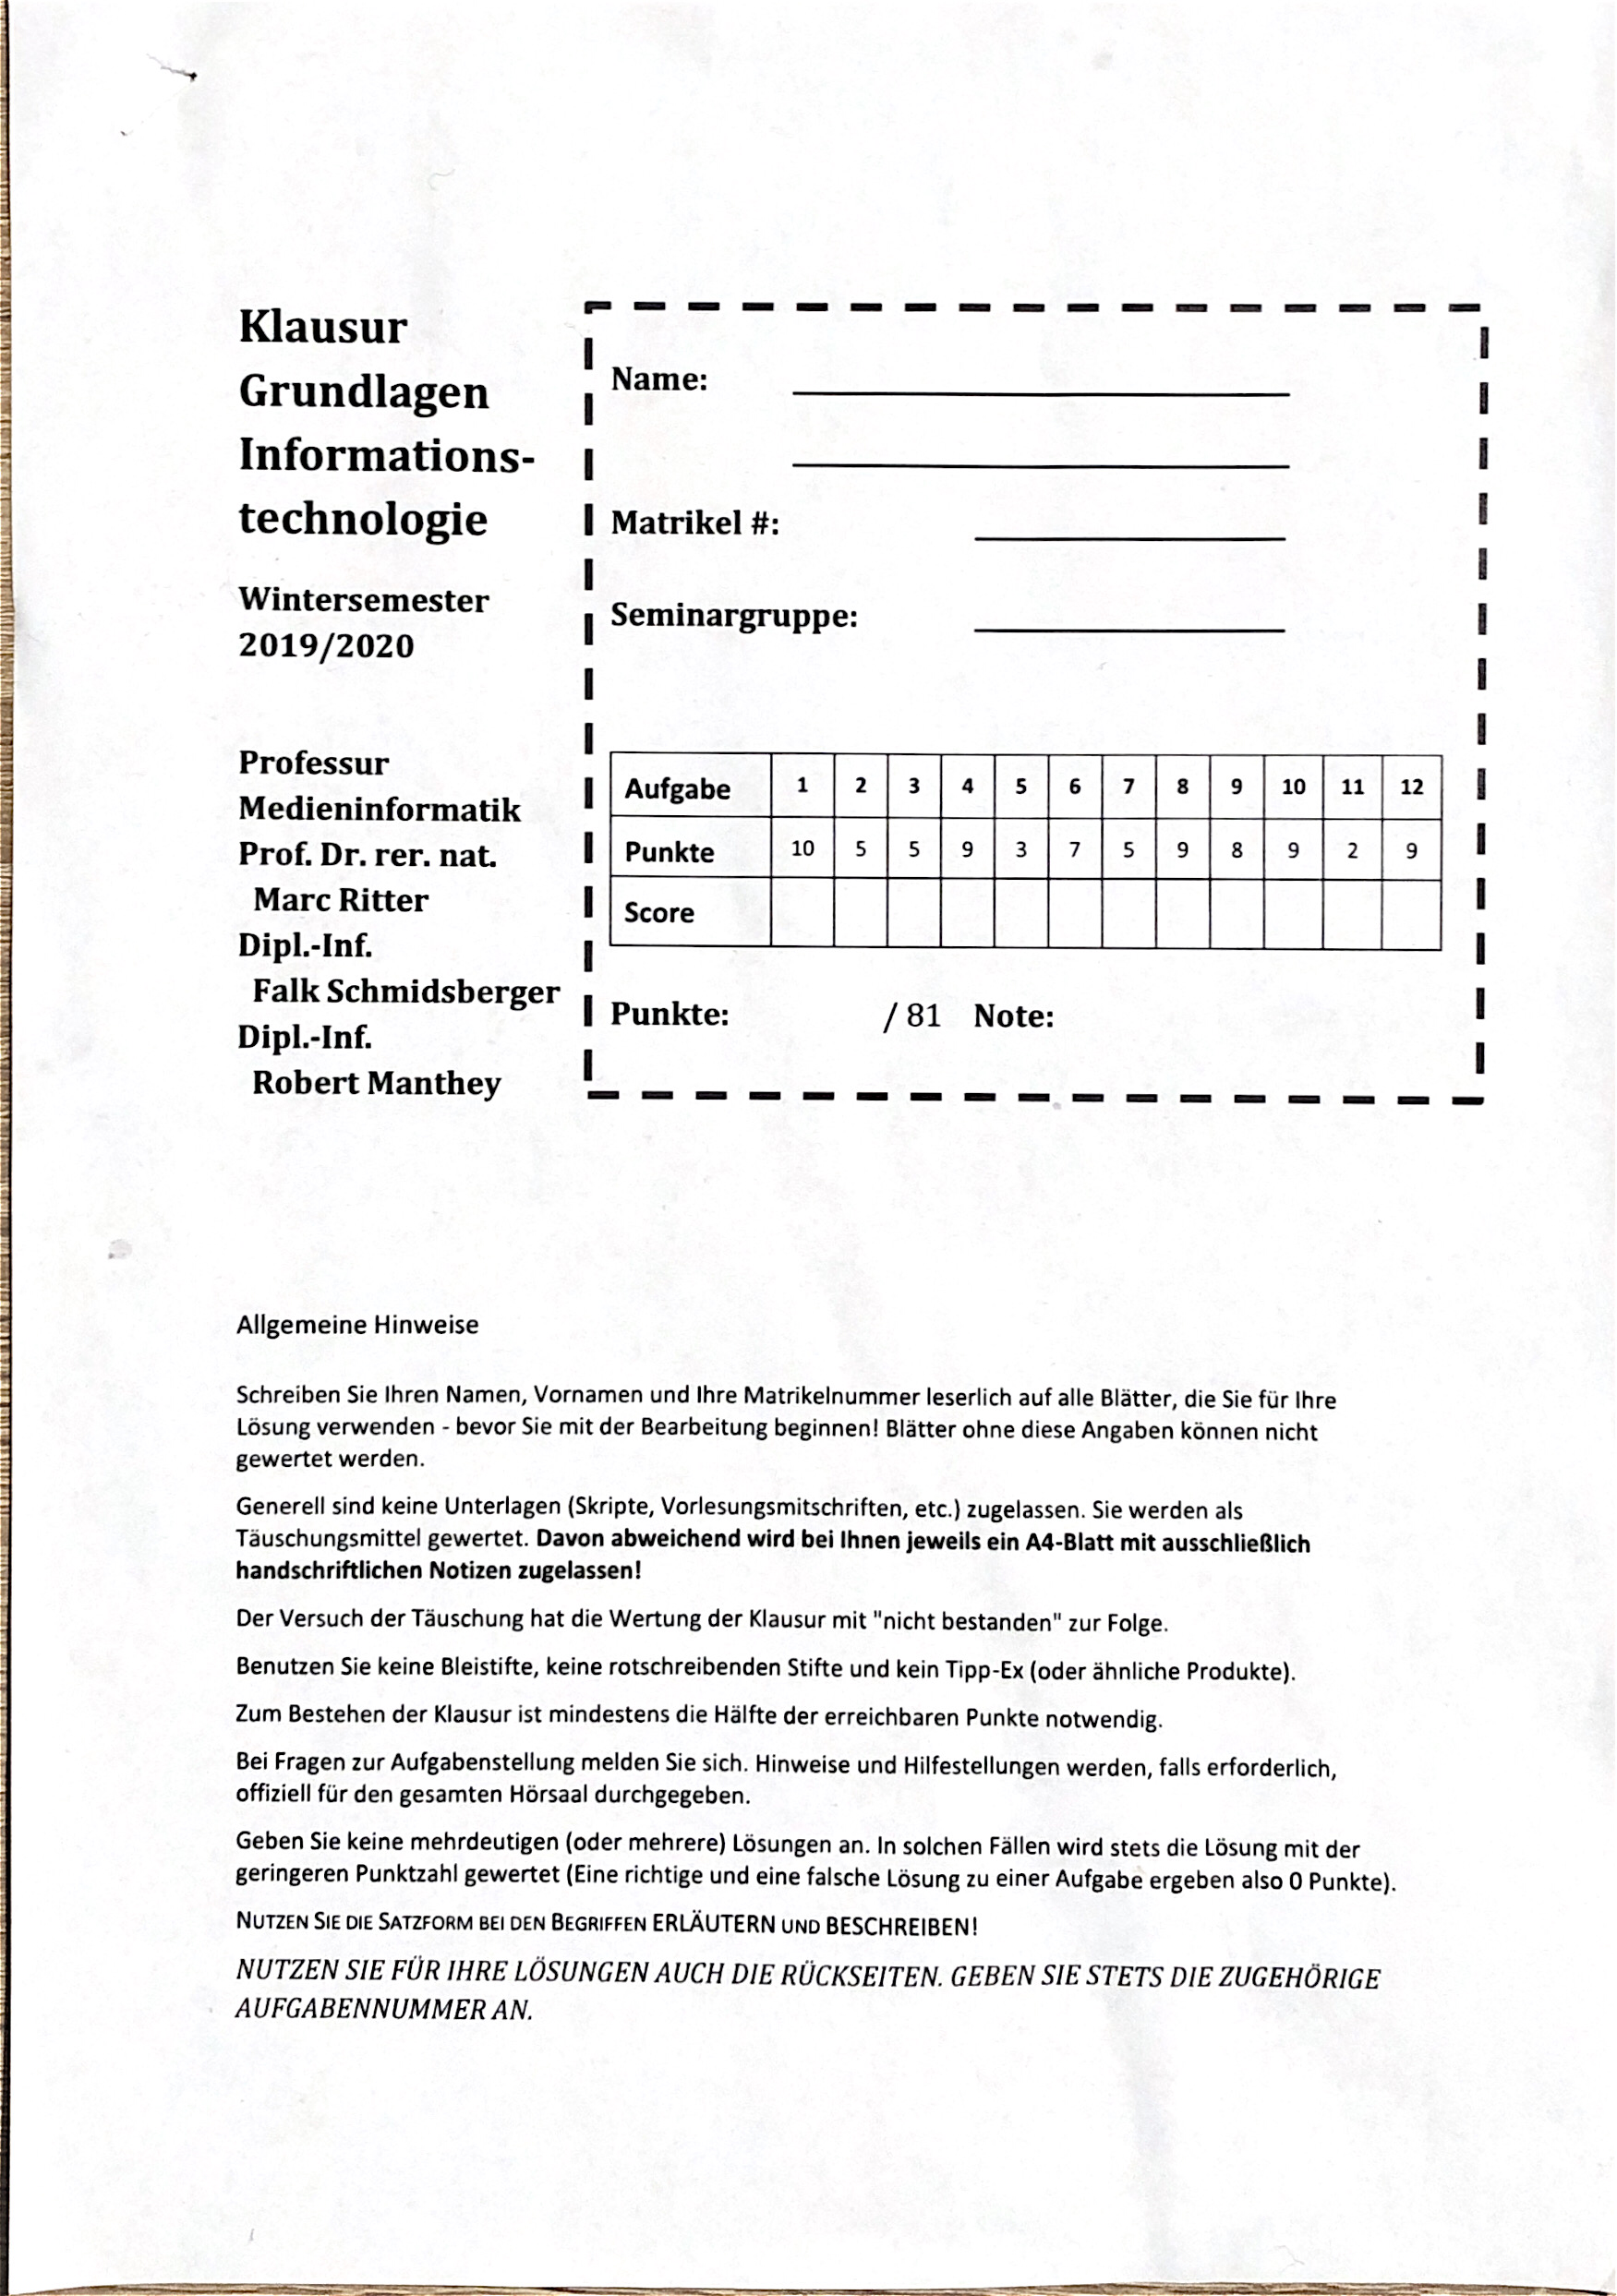
\includegraphics[width=0.96\textwidth]{img/seite1}}
       		\caption{Deckblatt der Klausur}
        	\label{fig:seite1}
    	\end{subfigure}
    	\begin{subfigure}[t]{0.4\textwidth}
        	\frame{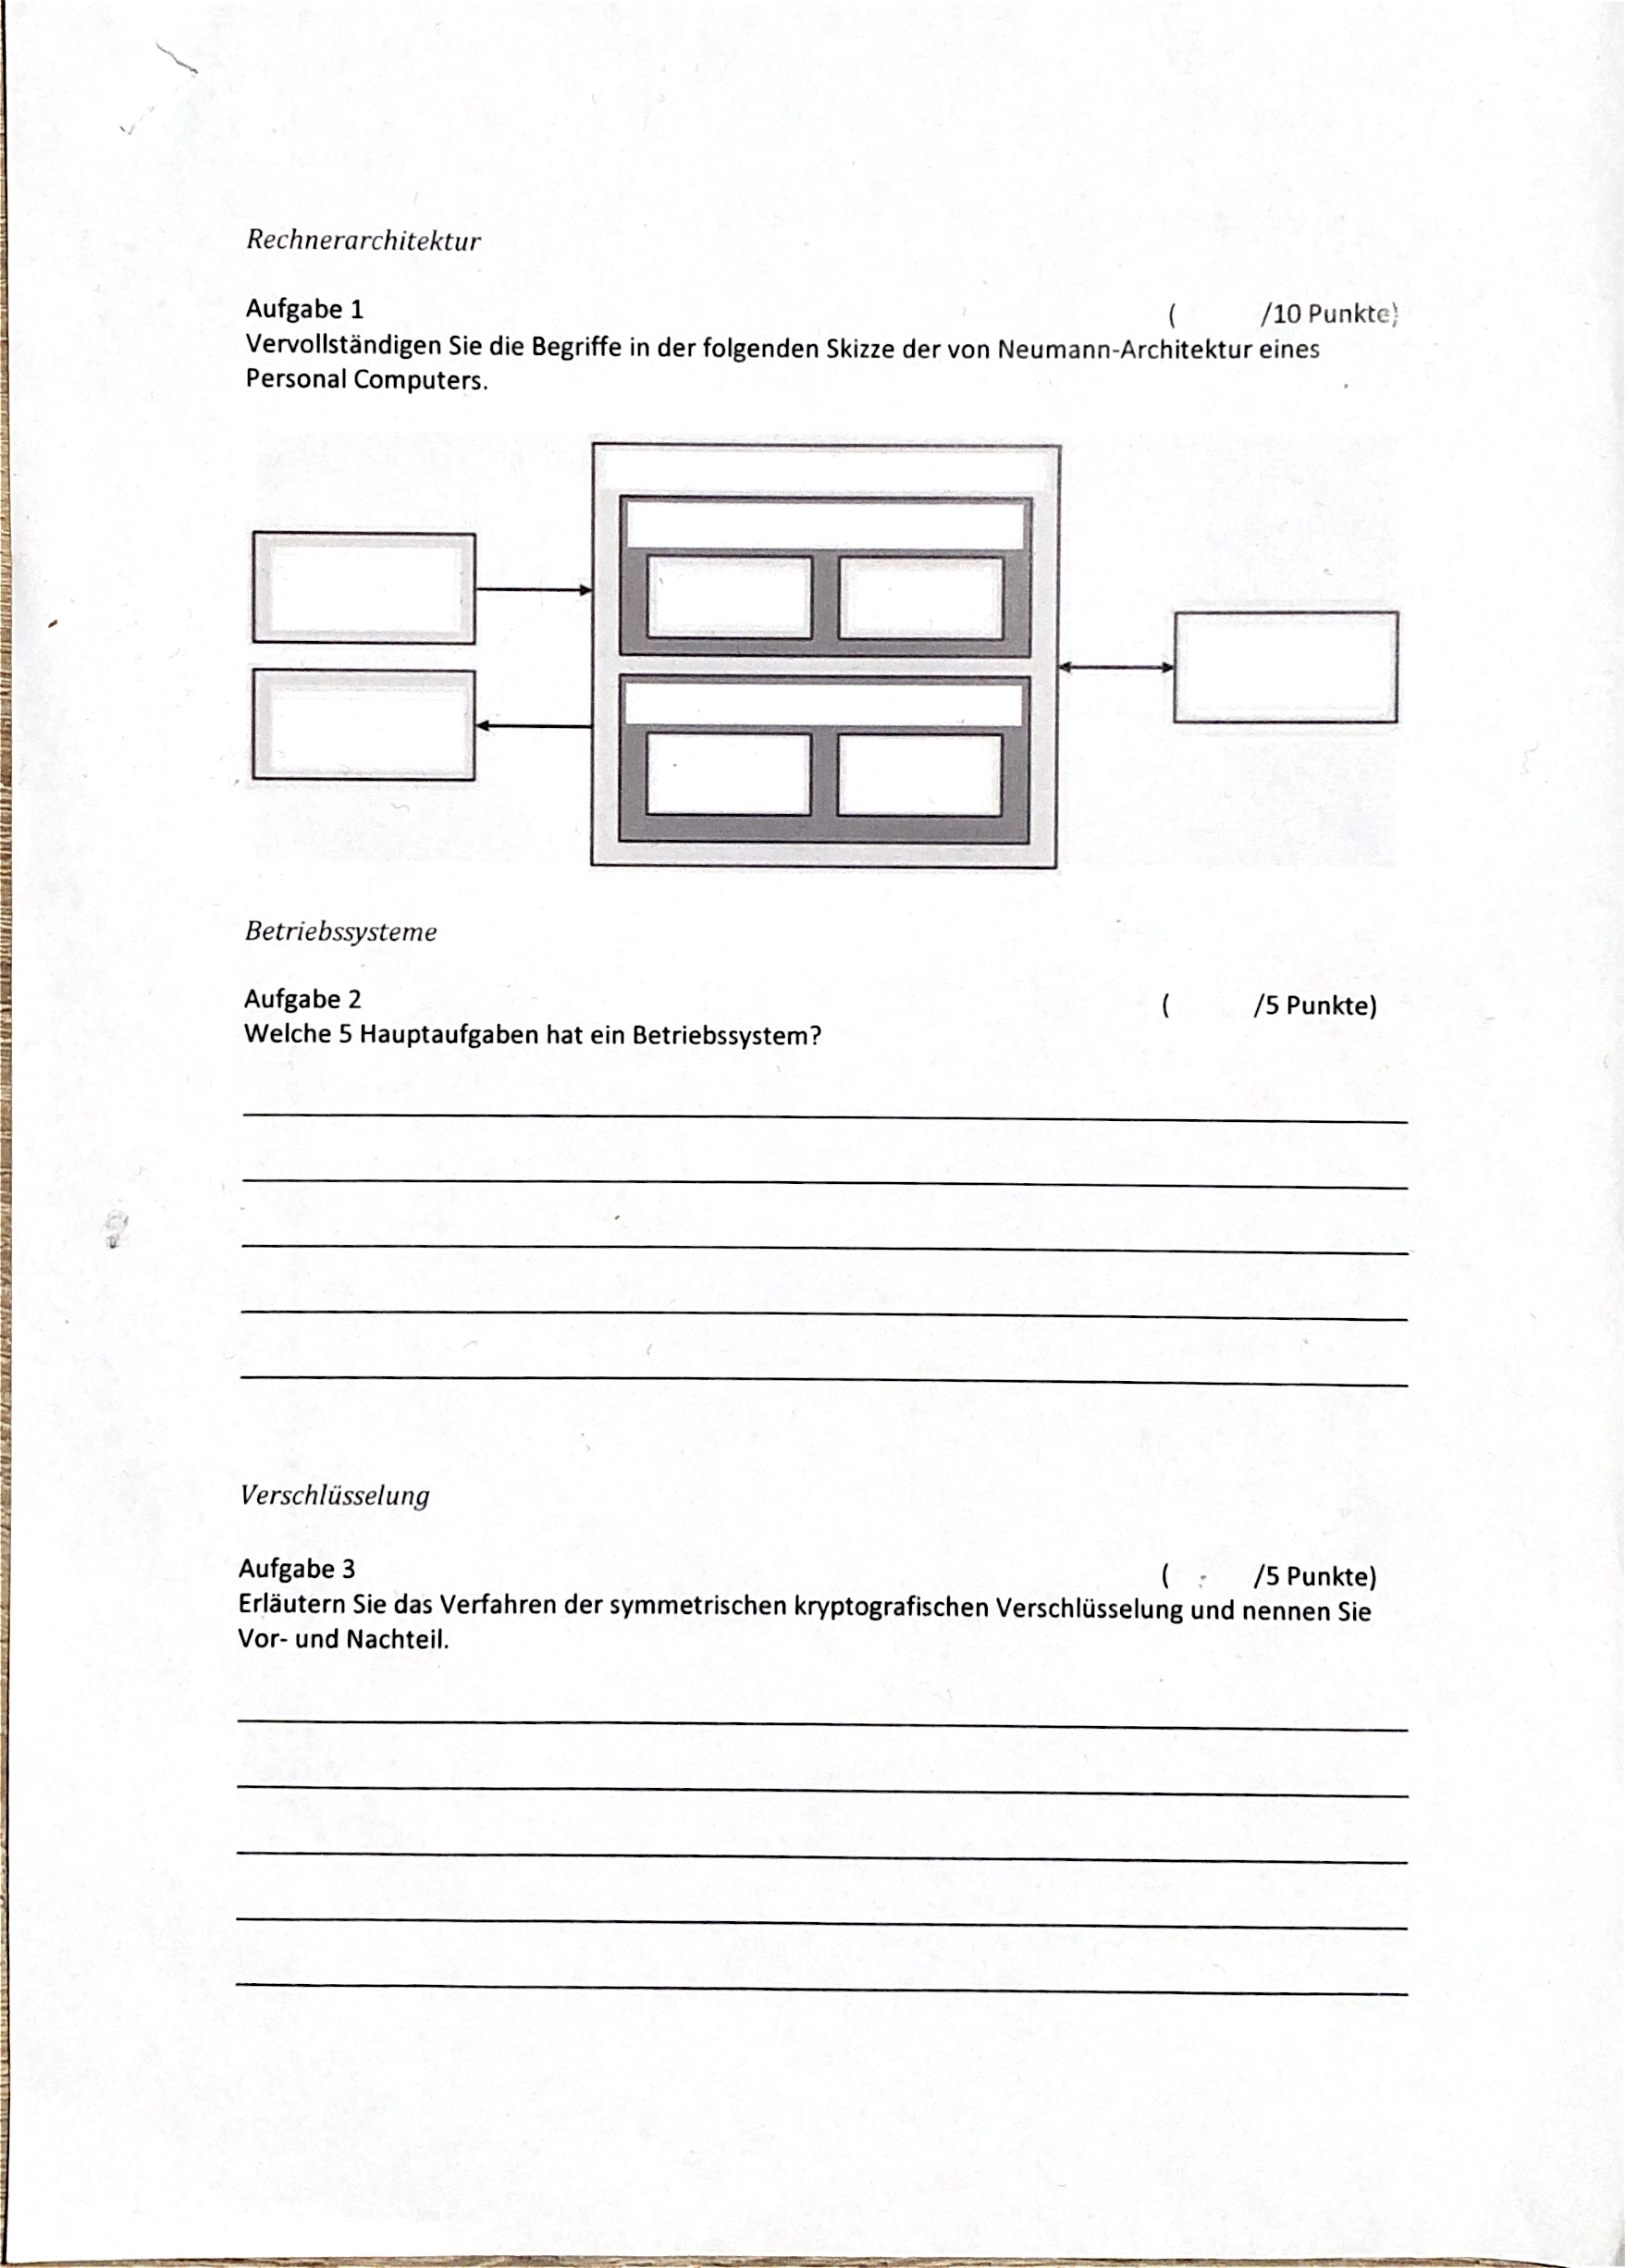
\includegraphics[width=0.96\textwidth]{img/seite2}}
        	\caption{Erste Seite der Klausur mit drei Aufgaben}
        	\label{fig:seite2}
    	\end{subfigure}
    	\caption{Umsetzung der Klausuren-Vorlage der Fakultät CB.}
    	\caption*{\textit{Die Bilder sind beim Erstellen einer Scan-Vorlage mit der App entstanden.}}
    	\label{fig:klausur}
	\end{figure}
	
	\section{Klausuren-Vorlage}\label{sc:klausuren-vorlage}
	Eine Klausuren-Vorlage bzw. ein Gestaltungsleitfaden für Klausuren der Fakultät \textit{Angewandte Computer- und Biowissenschaften} bietet außerdem die Möglichkeit der Kontrolle des Prüfers. Durch das vorgegebene Layout der Klausur ist es möglich, Fehler des Prüfers zu erkennen. Die Klausur in \autoref{fig:klausur} ist nach dieser Klausuren-Vorlage angefertigt worden. Auf dem Deckblatt (\ref{fig:seite1}) der Prüfung ist eine Tabelle, mit drei Zeilen und für jede Aufgabe eine Spalte. In der ersten Zeile befinden sich die Nummern der Aufgaben, in der zweiten die zu erreichenden Punkte der Aufgabe. Und in der dritten Zeile trägt der Prüfer die erbrachten Punkte des Studenten ein. Unter der Tabelle befindet sich ein Feld für die erreichte Gesamtpunktzahl sowie ein weiteres für die aus den Punkten resultierende Note. Es soll nun überprüft werden, ob die Summe der erreichten Punkte mit der Gesamtpunktzahl übereinstimmt und weiter soll auch die Note errechnet und mit dem Ergebnis der Prüfers verglichen werden. Eine weiteres Merkmal der Klausuren-Vorlage ist ein Feld, für die vom Studenten erreichten Punkte über jeder Aufgabenstellung auf den hinteren Seiten. Zu sehen sind solche Felder in \autoref{fig:seite2} am rechten Seitenrand. Die dortige Angabe sollte mit der, in der Tabelle auf dem Deckblatt (\ref{fig:seite1}) übereinstimmen und bietet somit noch eine weitere Möglichkeit der Kontrolle an.
	
	\section{Klausuren-Vorlage verbessern}
	Nachdem ein erster Prototyp zum Digitalisieren der Klausur-Daten entwickelt wurde, sollen außerdem Prüfungs-Vorlagen entstehen, die für die Digitalisierung optimiert sind. Dabei sollen Probleme, die beim Einscannen der aktuellen Vorlage erkannt wurden, behoben werden. 
	
	\section{Weitere Anmerkungen}
	Ferner soll bei der Problemlösung von der Anschaffung neuer Technologien und Geräte abgesehen werden. Grund dafür ist neben den Anschaffungskosten, die Idee, dass das Ergebnis des Forschungsprojekts in weiteren Lehr- und Forschungseinrichtungen Anwendung findet. Außerdem hat so gut wie jeder Mitarbeiter an einer Lehr- und Forschungseinrichtung ein eigenes oder Zugang zu einem Smartphone oder Tablet, welche durch die eingebaute Technik in der Lage sind, diese Aufgabe zu übernehmen. 

%%%%%%%%%%%%%%% - ANFORDERUNGEN - %%%%%%%%%%%%%%%

\chapter{Anforderungen}\label{ch:anforderungen}
	In diesem Kapitel wird erläutert, was die Anforderungen an das Software-System sind. 
%	Die hier aufgeführten Ideen entstanden während der Anforderungsplanung, wie im Kapitel \ref{ch:prototyp} nach zu lesen ist.

	Es soll eine App für das Betriebsystem iOS entstehen, mit der Klausuren digitalisiert werden können. Genauer müssen die, für die Notenfreigabe relevanten Daten der Klausur, in ein tabellarisches Format gebracht werden. Dazu soll die iOS-Anwendung Bilder von ausgefüllten Prüfungen aufnehmen können und den Inhalt mithilfe von Texterkennung digitalisieren. 
	
	Trotzdem nicht jede Klausur ein identisches Layout hat, soll die App in der Lage sein, alle relevanten Informationen, wie z. B. Name, Matrikelnummer und Note, richtig zu identifizieren und anschließend zu digitalisieren. Dafür soll der Benutzer digitale Vorlagen, sogenannte Scan-Vorlagen erstellen, durch die die App, die Informationen leichter findet und schneller digitalisiert, als wenn eine komplette Seite digitalisiert und analysiert werden müsste. 
	
	Zusätzlich soll es dem Benutzer möglich sein, Kontrollmechanismen fest zu legen. Wie im \autoref{sc:klausuren-vorlage} beschrieben, soll überprüft werden, ob die Punkte auf dem Deckblatt mit den Punkten auf den hinteren Seiten übereinstimmen und ob die Gesamtpunktzahl korrekt summiert wurde sowie die daraus resultierende Note richtig ist. Ein Kontrollmechanismus soll so gestaltet sein, dass die eben genannten Überprüfungsmöglichkeiten vom Benutzer selbst umgesetzte werden können. Beim Digitalisieren einer Klausur sollen so dem Benutzer Fehlermeldungen angezeigt werden, wenn bei der Überprüfung durch einen Kontrollmechanismus etwas falsch ist. Beispielsweise hat der Prüfer auf dem Deckblatt fünf Punkte eingetragen, bei der Aufgabenstellung auf den hinteren Seiten jedoch eine sechs. Die App  soll dann eine Fehlermeldung ausgeben, dass die Punktezahlen bei der Aufgabe nicht übereinstimmen und nochmals kontrolliert werden müssen. 
 
 	Zur Digitalisierung von Buchstaben soll Zeichen bzw. Texterkennung verwendet werden, die auf dem Gerät statt findet. Allerdings darf die App auch Texterkennung auf externen Servern unterstützen. Hierfür müssen dann die entsprechenden Server-Schnittstellen zur Kommunikation implementiert oder für einen eigenen Server entwickelt werden.

	Die digitalisierten Daten, die für die Texterkennung entstandenen Klausuren-Bilder und die erstellten digitalen Scan-Vorlagen sollen außerhalb der App auf einem Server gespeichert werden. Somit ist die Möglichkeit gegeben, die  Vorlagen wieder zu verwenden und anderen Benutzern der App zur Verfügung zu stellen. Aus den digitalisierten Daten sollen wiederum Tabellen entstehen, die an die Notenfreigabe weiter geben werden können.
	
	Damit Synchronität der Daten auf den Geräten und dem Server gewährleistet werden kann, benötig die App hierfür ebenfalls Schnittstellen. Diese sollten den standardmäßigen \textit{CRUD}\nomenclature{CRUD}{Das Akronym CRUD steht für Create/Erstellen, Read/Lesen, Update/Aktualisieren und Delete/Löschen und umfasst die vier grundlegenden Operationen persistenter Speicher}-Operationen entsprechen. 
	
	Da die gesamte Kommunikation über das Internet geschieht, muss das Softwaresystem den üblichen Datenschutz- und Datensicherheit-Richtlinien entsprechen, bzw. sie in der technischen Implementierung umsetzten. Für genauere Details zu den Sicherheitsmechanismen und den CRUD-Operationen zum Server siehe im Praktikumsbericht von Tobias Kallauke. 

%%%%%%%%%%%%%%% - GRUND IDEE ZUM LÖSEN DES PROBLEMS - %%%%%%%%%%%%%%%

\chapter{Konzept der Dokumenten-Scanner-App}\label{ch:konzept}
	Diesem Kapitel beschriebt, wie das Softwaresystem die Anforderungen umsetzt. Zur Erinnerung, die Dokumenten-Scanner App soll wichtige Daten auf dem Deckblatt (\ref{fig:seite1}) einer Klausur, wie Vor- und Nachname des Studenten, seine Matrikelnummer sowie die Note erkennen, digitalisieren und in ein für die Notenfreigabe geeignetes Format bringen. Die digitalisierten Daten sollen anschließend an einen Server gesendet werden, auf dem sie und die beim Einscannen entstandenen Bilder gespeichert werden. Verwendet eine einzuscannende Klausur die Klausuren-Vorlage (\ref{fig:klausur}) der Fakultät CB oder ähnliche Vorlagen, die eine Punkteübersicht haben, dann ist es außerdem möglich, die Punkte sowie die Note auf Richtigkeit zu überprüfen. 
	
	\section{Scan-Vorlage erstellen und speichern}
	
		Im folgenden Abschnitt wird zuerst verkürzt und anschließend detailliert geschildert, wie eine Scan-Vorlage zu erstellen ist.
	
		\begin{figure}[th]
    		\centering
    		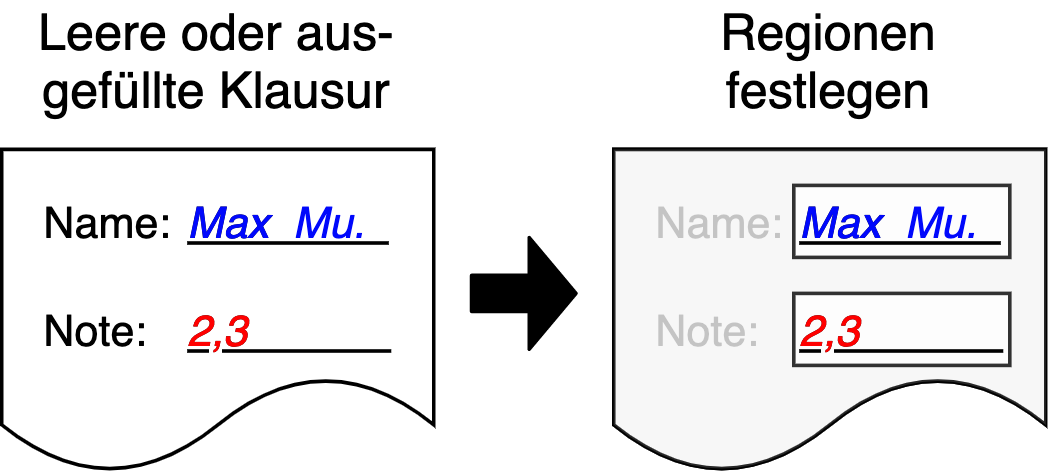
\includegraphics[width=0.6\textwidth]{img/schablone1}
    		\caption{Schematisches Schaubild zum Verständnis des Schablonen-Konzepts}
    		\label{fig:schablone1}
    	\end{figure}
    
		Um wirklich nur relevante Daten zu digitalisieren, benötig es die sogenannte Scan-Vorlage, die in der App angelegt werden kann. Eine Scan-Vorlagen funktioniert ähnliche, wie eine Schablone. Diese wird beispielsweise auf das Deckblatt gelegt, sodass nur noch die wichtigen Informationen, die digitalisiert werden sollen, zu sehen sind. Alles andere, was nicht von Interesse ist, wird von der Schablone überdeckt. In der \autoref{fig:schablone1} ist dieses Konzept schemahaft zu sehen. Aus dem analogen Beispiel abgeleitet, benötigt es zwei grobe Schritte, um eine  digitale Schablonen anzufertigen. Zuerst muss ein Foto von der Seite aufgenommen werden und anschließend müssen die Regionen eingezeichnet werden, die digitalisiert werden sollen. Eine Scan-Vorlage ist jedoch nicht nur eine einzige digitale Schablone sondern einer Sammlung aller zu einem Dokument. Denn jede Seite benötigt eine eigene individuelle.
	
		\begin{figure}[th]
    		\centering
    		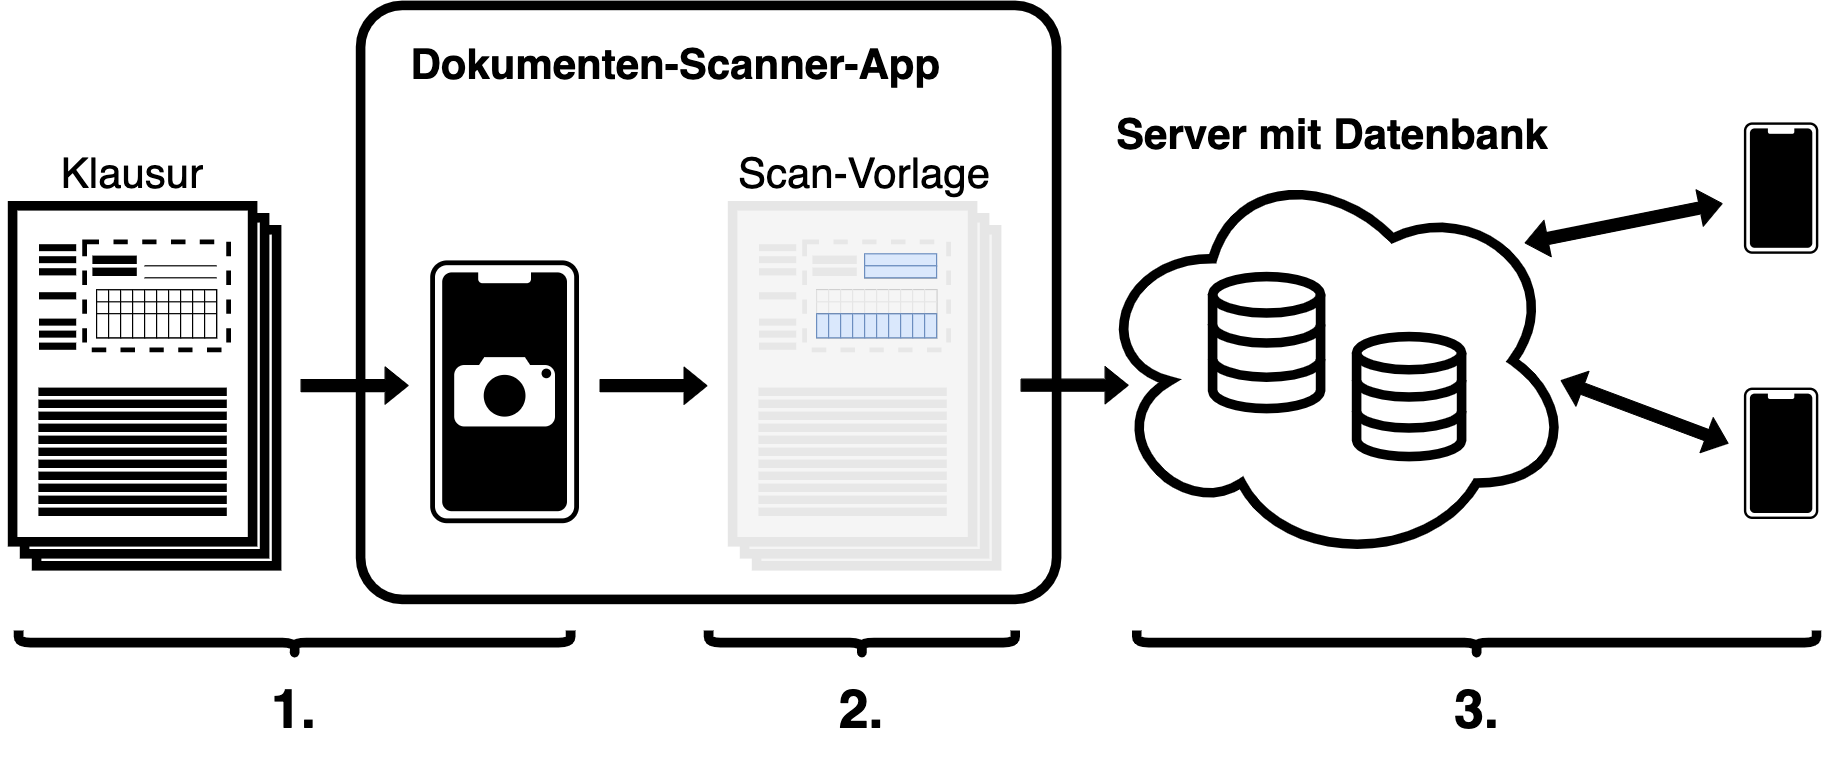
\includegraphics[width=\textwidth]{img/schema1}
    		\caption{Scan-Vorlage erstellen und auf dem Server speichern}
    		\label{fig:schema1}
    	\end{figure}
	
		In der folgenden Aufzählung wird nun detailliert beschrieben, wie die Abfolge beim Erstellen einer Scan-Vorlage ist. Der Vorgang ist in  \autoref{fig:schema1} schematisch dargestellt.
	
		\begin{enumerate}
			\item Zu Beginn wird jede Seite der Klausur fotografiert. Dabei wird in jedem Bild das Dokument erkannt, vom Hintergrund getrennt bzw. ausgeschnitten und perfekt ausgerichtet. Zudem wird der Kontrast erhöht, sodass die Schrift leichter lesbar wird. Die \autoref{fig:klausur} resultierte aus dem Prozess (siehe auch \autoref{fig:v3}). 
		
			\item Anschließend markiert der Benutzer diejenigen Regionen auf jeder Seite, die zu digitalisieren und/oder zu kontrollieren sind. In dem Schema \ref{fig:schema1} sind die Regionen blau hinterlegt (siehe auch \autoref{fig:v9}). Zusätzlich muss jeder Region eine Bezeichnung und einer der folgenden Datentypen zugeordnet werden: Unbekannt, Vorname, Nachname, Matrikelnummer, Seminargruppe, Punkte und Note (siehe auch \autoref{fig:v8} und \ref{fig:v9}). Die Angabe des Datentyps ist wichtig, da dadurch eindeutig wird, ob es sich um die Note oder den Vornamen des Studenten handelt. Diese Eindeutigkeit wird nicht nur für die automatische Erstellung der Tabelle benötigt, sondern auch für die Optimierung der Texterkennung. \label{it:zwei}
			
			\item Als letztes wird die Vorlage abgespeichert, welche dann automatisch an einen Server gesendet wird, so dass andere diese Vorlage ebenfalls benutzen können.
		\end{enumerate}
		%Kontrolle
 		Zusätzlich können in der Phase der Erstellung einer Scan-Vorlage die in \autoref{ch:anforderungen} beschriebenen Kontrollmechanismen festgelegt werden. Dies geschieht nach \autoref{it:zwei}, also nachdem alle Regionen angelegt wurden. Diese Kontrollmechanismen beruhen auf zwei simplen Konzepten. 

 		Das erste Konzept ist der Vergleich. Zur Erinnerung, es sollen die eigetragenen Punkte auf dem Deckblatt mit den Punkten neben der Aufgabenstellung auf den hinteren Seiten auf Gleichheit überprüft werden. Das zweite Konzept baut auf dem ersten auf. Statt einfach zwei Regionen bzw. Komponenten zu vergleichen, wird eine oder werden beide zuvor berechnet. Beispielsweise soll die Summe der Teilaufgaben mit Gesamtpunktzahl übereinstimmen. Das bedeutet, es wird erst die Summe berechnet und anschließend mit der vom Prüfer eingetragenen Punktzahl verglichen. Oder aber die Gesamtpunktzahl wird in die Note umgerechnet und mit der vom Prüfer eingetragen Note verglichen. 
 	
 		Beim festlegen der Kontrollmechanismen wird wie folgt vorgegangen:
 		\begin{enumerate}
 			\item Der Benutzer wählt ein Kontrollmechanismus aus. Zur Auswahl stehen, entweder \textit{zwei Regionen}, \textit{die Gesamtpunktzahl} oder \textit{die Note} vergleichen. 
 			\item Aus den zuvor angelegten Regionen müssen nun die passenden Regionen ausgewählt werden. Abhängig von dem ausgewählten Kontrollmechanismus geben die beiden zu vergleichende Komponente dem Benutzer Auskunft darüber, welche und wie viele Regionen auszuwählen sind.
 			\item Der Kontrollmechanismus kann gespeichert werden, sobald in jeder zu vergleichenden Komponente die Mindestzahl an auszuwählenden Regionen erreicht wurde. Diese werden in der Scan-Vorlage hinterlegt und mit an den Server gesendet, sodass alle Benutzer bei den Vorlagen die selben Kontrollmechanismen besitzen.
 		\end{enumerate}
 		
 	\section{Scan-Vorlage verwenden}
 	
 		Im folgenden Abschnitt wird zuerst verkürzt und anschließend detailliert geschildert, wie eine erstellte Scan-Vorlage zu verwenden ist und wie diese funktioniert.
 	
 		\begin{figure}[th]
    		\centering
    		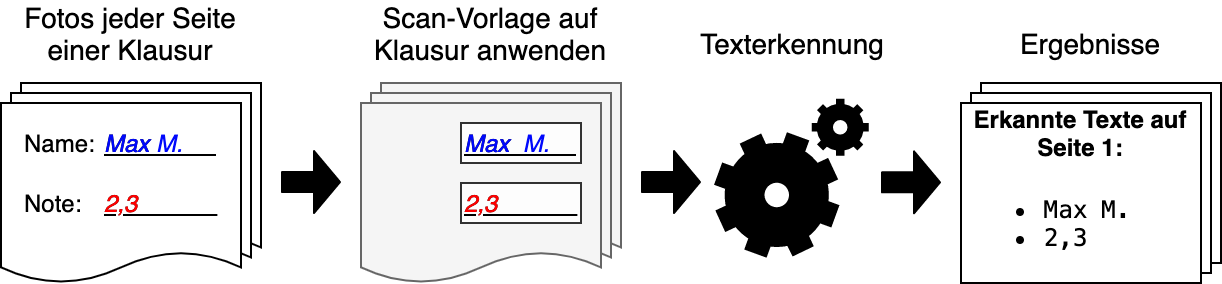
\includegraphics[width=\textwidth]{img/schablone2}
    		\caption{Schematischer Ablauf beim Verwenden einer Scan-Vorlage}
    		\label{fig:schablone2}
    	\end{figure}
 
 		Nach dem Erstellen einer Scan-Vorlage kann diese auf ausgefüllten Klausuren angewandt werden. In \autoref{fig:schablone2} wird der Ablauf schematisch dargestellt. Zuerst werden die ausgefüllten Prüfungs-Seiten einer Klausur fotografiert. Anschließend stellen die digitalen Schablonen die relevanten Informationen jeder Seite für den nächsten Schritt bereit. Optical character recognition (OCR)\nomenclature{OCR}{optical character recognition, deutsch: optische Zeichenerkennung und im deutschen Synonym für Texterkennung}, auf deutsch optische Zeichenerkennung, wird dazu benutzt, die Daten aus den Schablonen zu digitalisieren. 
		
		\begin{figure}[th]
    		\centering
    		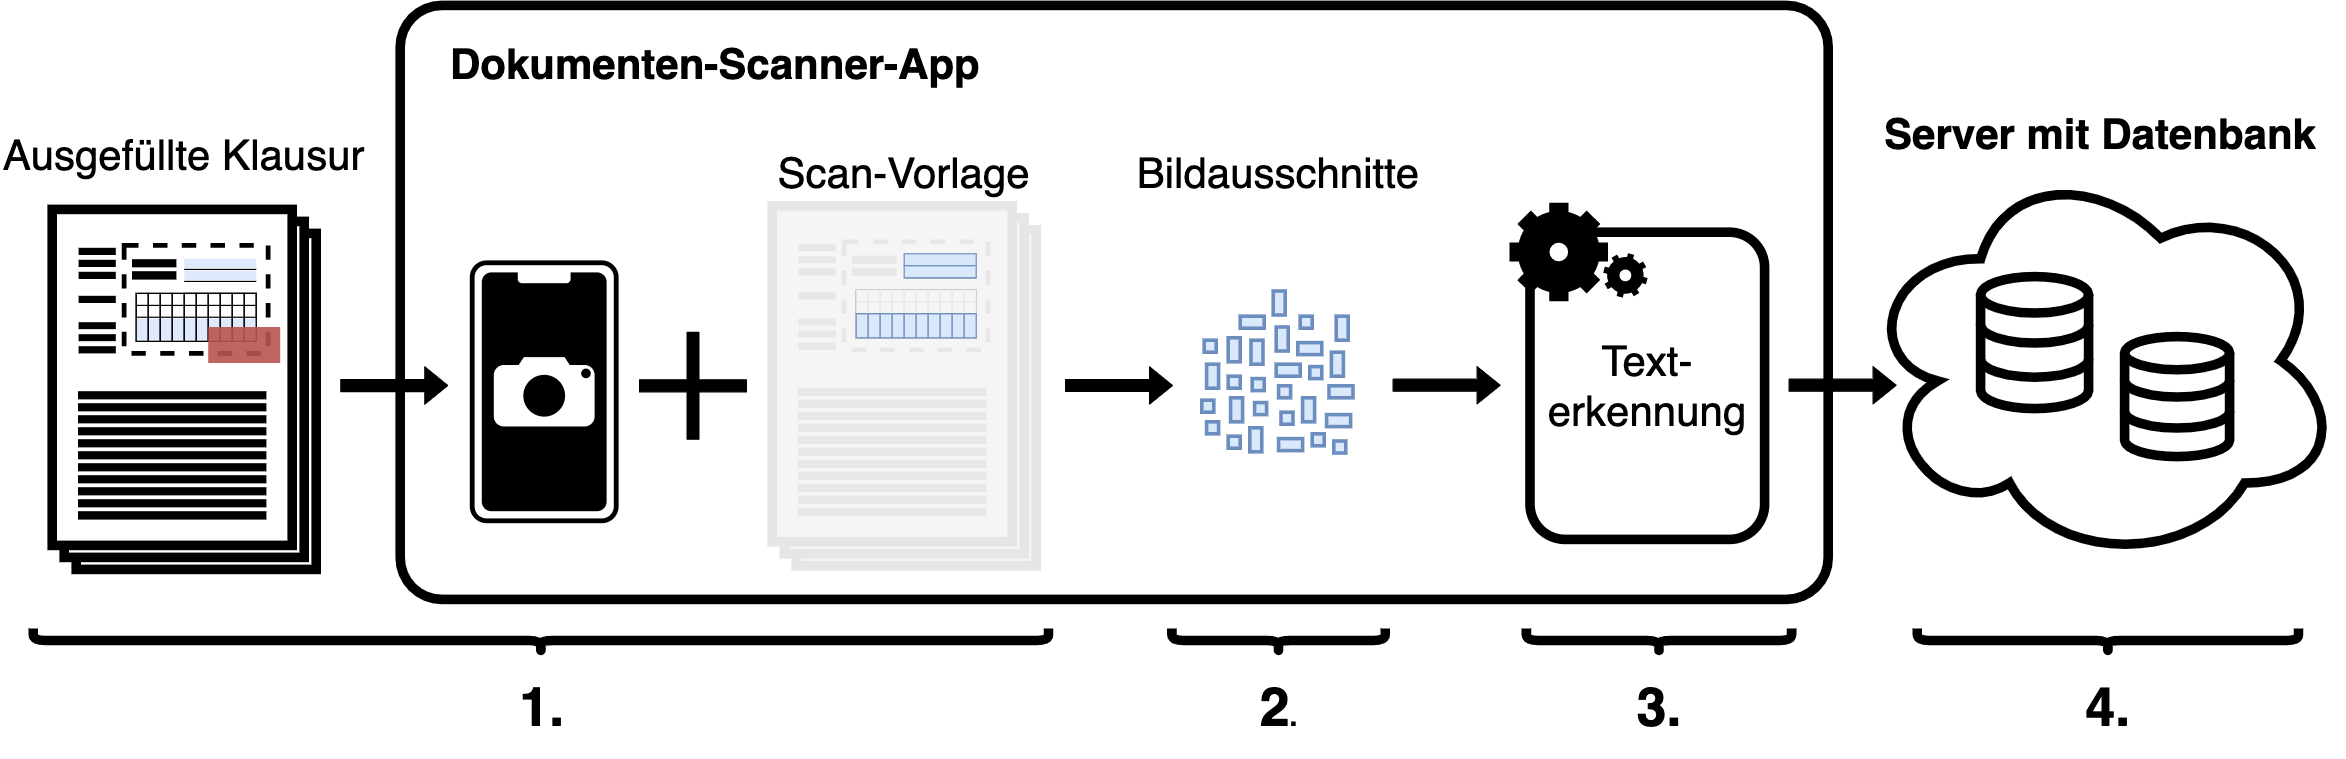
\includegraphics[width=\textwidth]{img/schema2}
    		\caption{Scan-Vorlage verwenden}
    		\label{fig:schema2}
    	\end{figure}
    	
    	In der folgenden Aufzählung wird detailliert beschrieben, wie die Abfolge beim Verwenden einer Scan-Vorlage ist. Der Vorgang ist in \autoref{fig:schema2} schematisch dargestellt.
	
		\begin{enumerate}
			\item Die Seiten der Klausur müssen zuerst in derselben Reihenfolge, wie in der Scan-Vorlage fotografiert werden. Anschließend werden die Regionen der Scan-Vorlage auf das jeweilige Bild angewendet. Bei dem Prozess entstehen Bildausschnitte, in denen die relevanten Informationen enthalten sind.
			\item Die entstandenen Bildausschnitte werden Seitenweise in die Texterkennung überführt.
			\item Die App digitalisiert mithilfe von OCR den Inhalt der Ausschnitte. Der Datentyp der zugehörigen Region aus der Scan-Vorlage nimmt nun Einfluss auf das Ergebnis. Durch ihn wird während der Worterkennungsphase eine Liste an vordefinierten möglichen Ergebnissen eingespeist. Diese Liste hat Vorrang vor dem sogenannten Standard-Wörterbuch und verbessert dadurch die Texterkennung. Ein Beispiel für solch eine Liste könnten, alle möglichen Noten sein. Auch vorstellbar ist, dass alle Seminargruppen oder Namen von Personen, die an der Klausur teilgenommen haben, dort verwendet werden.
			\item Die Ergebnisse werden im Anschluss an den Server gesendet. Zuvor kann der Benutzer jedoch die Ergebnisse anpassen bzw. korrigieren, falls es bei der Texterkennung zu Fehlern kam. Auch die Kontrollmechanismen finden vor dem Upload zum Server statt und geben dem Nutzer durch Fehlermeldungen Hinweise. \label{it:senden}
		\end{enumerate}
		
	\section{Erweiterung des Konzepts}\label{sc:erweiterungkonzept}
		Weiter ist eine zusätzliche Möglichkeit der Korrektur sinnvoll. Angenommen, jemand verschreibt sich bei seiner Seminargruppe und vergisst ein Zeichen. Die Texterkennung erkennt zwar jedes Zeichen richtig, jedoch ist das Ergebnis keine korrekte Seminargruppe. Deshalb sollte im Nachhinein an die Texterkennung das Ergebnis mit einer richtigen Seminargruppe, die die größte Übereinstimmung mit dem erkannten Wort hat, ersetzt werden. Bei diesem Vorgehen ist zu beachten, dass nur die Seminargruppen verwendet werden, die tatsächlich die Klausur geschrieben haben. Ähnliches gilt wieder für die Namen oder Matrikelnummern der Studenten.
		
		Allerdings entstehen auch durch das OCR Fehler. Aus diesem Grund ist die sogenannte confidence neben jedem Ergebnis sichtbar. Diese sagt aus, wie sicher sich die Texterkennung bei dem Ergebnis ist. Jedoch kann es auch hier falsche Positiv-Ergebnisse geben, weshalb auch das kein perfekter Indikator für die Richtigkeit ist. Deshalb gibt es, wie im \autoref{ch:konzept} \autoref{it:senden} schon beschreiben, die Möglichkeit, die Ergebnisse noch einmal zu überprüfen und zu korrigieren, bevor sie an den Server zum Abspeichern gesendet werden. Auch die Kontrollmechanismen reagieren auf die Änderungen der Ergebnisse, sodass Fehlermeldungen behoben werden können. 

%%%%%%%%%%%%%%% - PROTOTYP - %%%%%%%%%%%%%%%

\chapter{Entwicklung des ersten Prototyps}\label{ch:prototyp}
	Dieses Kapitel beschreibt die Entwicklung der iOS-App in einer ähnlichen Reihenfolge, wie das bekannte Wasserfall-Model über die Verwaltung der Entwicklung großer Softwaresysteme nach Winston W. Royce \cite{royce_managing_1970}.
	
	\section{Anforderungsplanung}\label{sc:anforderungsplanung}
	Vor Beginn des Praktikums wurde diskutiert und kalkuliert, welches Thema aus dem Projekt Memo Space für ein zwölfwöchiges Praktikum geeignet ist. Dabei entstand eine Art Durchführbarkeits- / Machbarkeitsstudie, welche zur Entscheidung führte, ein Dokumenten-Scanner-Softwaresystem umzusetzen. Aufgrund der Kenntnisse und Erfahrung, soll ein Backend mit entsprechenden Schnittstellen und eine Android-App von Tobias Kallauke umgesetzt werden, währende vom Verfasser eine iOS-App gefordert ist. Die iOS-Anwendung soll den Anforderungen, die im gleichnamigen \autoref{ch:anforderungen} zu finden sind, erfüllen. Für weitere Details über den Server und die Android-App siehe im Praktikumsbericht von Tobias Kallauke.

	\section{Planung und Vorbereitung bzw. Analyse und Definition}\label{sc:analyse}
		Die Aufgaben bzw. Ziele dieser Phase sind: \begin{enumerate}
			\item die Auseinandersetzung mit der Problemstellung und den Anforderungen,
			\item das Betreiben von einer Problemanalyse,
			\item die Entwicklung von Ideen und eines genauen Konzepts der iOS-App sowie 
			\item das Entwickeln eines ersten minimalen Prototyps, als Machbarkeitsnachweis.
		\end{enumerate}
		
		Bei der Entstehung des Konzepts, welches im \autoref{ch:konzept} zu finden ist, spielen die Dokumentationen der Frameworks \textit{Vision}\footurl{Dokumentation von Vision -}{https://developer.apple.com/documentation/vision} , \textit{VisionKit}\footurl{Dokumentation von VisionKit -}{https://developer.apple.com/documentation/visionkit} und \textit{PhotoKit}\footurl{Dokumentation von PhotoKit -}{https://developer.apple.com/documentation/photokit} von \textit{Apple} eine entscheidende Rolle. Aus ihnen wird klar, welche Funktionen der App noch zu entwickeln und welche in Frameworks schon vorhanden sind. Z. B. ist das Erkennen und das gerade Ziehen von Dokumenten in Echtzeit, sowie die Texterkennung auf Bildern in \textit{Vision} und \textit{VisionKit} enthalten. Bei der Entwicklung des ersten Prototyps half eine Beispiel-App von \textit{Apple} \cite{apple_detecting_2019}, die das Erkennen von Objekten in Standbildern mithilfe der genannten Frameworks umsetzt.
		
		Durch die Auseinandersetzung mit den Bibliotheken konnte festgestellt werden, dass die zu entwickelnde App nur Geräte mit iOS 13.0 oder neuer unterstützen werden kann. Grund dafür sind die \textit{Apple} Frameworks \textit{SwiftUI} und \textit{VisionKit}. \textit{SwiftUI} bietet die Möglichkeit, Benutzeroberflächen für alle \textit{Apple}-Plattformen in der Programmiersprache \textit{Swift} zu erstellen. Die deklarative \textit{Swift}-Syntax ist einfach zu lesen und schnell zu schreiben, so dass es möglich ist, die App in wenigen Wochen für iPhone und iPad zu entwickeln. Als Alternative gibt es noch \textit{UIKit} oder auch \textit{AppKit}, die unter alle iOS Versionen funktioniere. Diese Frameworks sind allerdings nicht deklarativ sodass, Views sowohl im Code als auch in Interface-Dateien getrennt voneinander erstellt und konfiguriert werden müssen \cite{sillmann_einstieg_2019}. Dadurch dauert die Entwicklung einer App, im Gegensatz zu SwiftUI deutlich länger, wie man auch hier in dem Video\footurl{SwiftUI vs UIKit – Comparison of building the same app in each framework -}{https://www.youtube.com/watch?v=qk2y-TiLDZo} von Paul Hudson einem in der Swift-Community sehr bekannten Programmiere und Autor sieht. Sehr ähnliche Erfahrung hat der Verfasser vor dem Praktikum in seiner Freizeit mit den beiden Frameworks gemacht. \textit{VisionKit} dagegen, ist das Framework zum Scannen der Dokumente. Auch hierfür gibt es eine Alternative. Das Framework ist von den Entwicklern von \textit{WeTransfer} und funktioniert auch auf älteren iOS Versionen. Allerdings unterstützt \textit{WeScan}\footurl{WeScan GitHub Repository -}{https://github.com/WeTransfer/WeScan} noch kein stapelweises Scannen. Das bedeutet, man kann immer nur ein Foto machen, welches erst abgespeichert werden muss, bevor man das nächste machen kann. Das ist für den Benutzer nicht bequem und spart wahrscheinlich auch keine Zeit. Zu Informationen zu anderen verwendeten Frameworks siehe im \autoref{ch:prototyp} \autoref{sc:implementierung}.

		Abschließend zu dieser Phase ist zu erwähnen, dass das Scrum-Konzept\footurl{Der Scrum Guide™ -}{https://www.scrumguides.org/scrum-guide.html}, welches sich für agile Softwareentwicklung anbietet, zur Projektplanung und zum Projektmanagement verwendet wurde. Als Versionsverwaltung der Software wurde Git\footurl{Git Internetseite -}{https://git-scm.com/} in Kombination mit GitHub Issues\footurl{Mastering Issues -}{https://guides.github.com/features/issues/} und GitHub Project Boards als Planungstools benutzt. So konnte der Verfasser selbständig jedem so genannten Sprint Aufgaben zuordnen und den Fortschritt nachvollziehen.

	\section{Grundlagen}
			In den folgenden zwei Absätze werden wichtige Konzepte und Grundwissen vermittelt, die im folgenden \autoref{ch:entwurfunddesign} Entwurf und Design nochmal aufgegriffen werden.

		\paragraph*{Model-View-ViewModel}
			Das sogenannte Entwurfsmuster Model View ViewModel (MVVM)\nomenclature{MVVM}{Model View ViewModel} entstand bei \textit{Microsoft} im Jahr 2005 mit der \textit{Windows Presentation Foundation} (WPF) und \textit{Silverlight-Technologien}. Ein Entwurfsmuster ist eine bewährte Lösungsvorlage für wiederkehrende Entwurfsprobleme. MVVM verwendet das Konzept eines Schichtmodells und ist eine abstrakte Darstellung einer Benutzeroberfläche, in Form einer Datenstruktur. Diese enthält Daten, die auf der Benutzeroberfläche angezeigt werden sollen und Anweisungen, die auf der Benutzeroberfläche aufgerufen werden können. Dieses sogenannte ViewModel, weiß nichts von Views, wie es sonst bei anderen Entwurfsmustern üblich ist, um Daten auf der Benutzeroberfläche anzuzeigen. Stattdessen verwendet eine MVVM-View eine Bindungsfunktion (data binging) zur bidirektionalen Zuordnung von Daten aus dem ViewModel zu den jeweiligen Eigenschaften auf der View. Z. B. Einträge in einer Dropdown-Menü. Aber auch das binden von Daten aus dem Model zu Benutzereingaben durch Maus, Tastatur oder Touch-Screens ist möglich. Beispielsweise kann ein Mausklick eine Anweisung in dem ViewModel auslösen. Diese verändert einen Wert im Model, wodurch die View durch data binding aktualisiert wird. \cite{papa_fundamental_2011} \cite{freeman_pro_2017} \cite{bragge_model-view-controller_2013}

		\paragraph*{Redux.js}
			Redux.js ist eine Bibliothek\footurl{Redux.js Github Repository -}{https://github.com/reduxjs/redux} für die Programmiersprache JavaScript. Diese stellt einen sogenannten vorhersehbaren Zustandscontainer\footurl{Redux Core Concepts -}{https://redux.js.org/introduction/core-concepts} für JavaScript Anwendungen bereit. In diesem Container wird der Zustand der gesamten Anwendung in einem Objektbaum innerhalb eines einzigen Speichers gespeichert. Diesen Baum kann man sich vorstellen, wie eine Matrjoschka die weitere Puppen in sich hat. Der wichtige Unterschied zwischen einer Matrjoschka und einem Baum ist jedoch, dass in eine Puppe genau nur eine andere gesteckt werden kann. Bei einem Objektbaum hingegen können mehrere Objekte nebeneinander in ein Objekt ''gesteckt'' werden und so weiter. Im Bezug auf einen Zustandscontainer enthält dieser dann States (Objekte) auf deutsch Zustände und Daten, die unteranderem auf der Benutzeroberfläche angezeigt werden sollen. Diese Aufteilung in die States ist dazu gedacht, einer View oder mehrere zusammenhängende Views nur die wirklich benötigten Daten bereit zustellen. Diese Struktur erleichtert das Testen oder Untersuchen der Anwendung und ermöglicht es, durch hinzufügen eines neuen States den aktuellen Entwicklungsstand der Anwendung beizubehalten und dadurch den Entwicklungsprozess zu beschleunigen. \\
			Ein weiteres wichtiges Prinzip\footurl{Redux Three Principles -}{https://redux.js.org/introduction/three-principles} von Redux ist, dass die Daten in den States Schreibgeschütz sind. Die einzige Möglichkeit den Zustand zu ändern, besteht darin, eine Aktion auszulösen, die beschreibt, was passiert. Dadurch wird sichergestellt, dass weder die Views noch Netzwerk-Rückrufe jemals direkt an den Zustand ändern können. Stattdessen bringen sie nur die Absicht zum Ausdruck, den Zustand zu verändern und lösen eine Aktion aus. Da alle Änderungen zentralisiert sind und eine nach der anderen in einer strikten Reihenfolge erfolgen, gibt es weniger Programmfehler-Quellen.

	\section{Entwurf und Design}\label{ch:entwurfunddesign}
		
		Eine typische Aufgabe dieser Entwurfsphase ist die Entscheidung über die Datenhaltung, die Verteilung im Netz und die Benutzeroberfläche des Software-Systems\footurl{Vorlesung 9, Folie 27 aus Softwaretechnik Grundlagen von Prof. Dr.-Ing. Wilfried Schubert (2019) -}{https://www.staff.hs-mittweida.de/~wschub/intranet/ss19/Fach_SWT/Fach_SWT_Zeitplan.htm}. Jedoch standen diese Grundsatzentscheidungen schon zu Beginn des Praktikums, durch die Kenntnisse von Tobias Kallauke und dem Verfasser fest. Der Server verwendet zur Datenspeicherung PostgreSQL\footurl{PostgreSQL Internetseite -}{https://www.postgresql.org/}, eine relationale Datenbank, sowie das Dateiverzeichnis für Bilder, während die App keine Daten persistent speichert. Durch die Aufteilung von App und Server handelt es sich um eine sogenannte Client/Server-Architektur. Für die Benutzeroberfläche der iOS-App wird, wie schon erwähnt, das deklarative SwiftUI verwendet. Weitere Informationen zum Backend und der Android-App befinden sich im Praktikumsbericht von Tobias Kallauke.
		
		Jedoch mussten noch Arbeit in den Workflow und in die Architektur der App gesteckt werden. Zur Definition einzelner Teil-Workflows, die zusammenhängende Aufgaben umfassen, wurden eine Art Zustandsautomaten bzw. Flussdiagramm beschrieben. Ein Beispiel, was noch einmal geändert in der App verwendet wurde befindet sich im \autoref{ch:workflow}. Die Modelle halfen dabei Views zu entwickeln und deren Design festzulegen. Das Aussehen der App sollten sich jedoch im Laufe der Zeit noch ändern, denn ersteinmal stand die Umsetzung des Konzepts im Vordergrund.

		Aus den Designs und den Teil-Workflows heraus entstand ein grober Plan, wie die Daten in der App gehandhabt werden sollten. Da \textit{SwiftUI} das Entwurfsmuster MVVM umsetzt, benötigt es eine Struktur für das ViewModel und für den Datenfluss der asynchronen Server-Rückrufe. Jedoch stellte sich die Entwicklung dieser Strukturen, auch schon während des allerersten Prototyps, als problematisch heraus. Denn auch bei steigender Komplexität soll das ViewModel noch übersichtlich bleiben, um eine schnelle Weiterentwicklung zu gewährleisten. Aus diesen Gründen begann die Suche nach einer besseren Lösung, bei der die JavaScript-Bibliothek \textit{Redux.js} zur Verwaltung von Zustandsinformationen in Webanwendung entdeckt wurde. 

		\textit{Redux} hilft durch dessen Konzept, komplexe Views mit vielen Daten schnell und einfach zu implementieren. Auch werden so Serverantworten und zwischengespeicherte Daten sowie lokal erstellte Daten, die noch nicht auf dem Server gespeichert wurden, strukturiert und zentral abgelegt. Das erleichtert nicht nur das Wiederverwenden von Daten, sondern spart auch wiederholte Server-Aufrufe ein. Es erschien nun möglich, trotz der begrenzten Zeit im Praktikum, möglichst viel mit wenig Fehlern umzusetzen. Denn Redux ermöglicht durch die modulare Aufteilung des State Containers eine schnelle Weiterentwicklung der App, auch wenn die Komplexität der Anwendung steigt. Und die Vorteile von Redux hinsichtlich des Testens und Untersuchens der App sollten helfen, Fehler möglichst schnell ausfindig zu machen, trotz asynchroner Programmabschnitte.

		Daher lag es nah die wesentlichen Konzepte von \textit{Redux} umzusetzen und einen \textit{Redux} ähnlichen State Container, als ViewModel zu implementieren. Aus der Definition von Teil-Workflows sollte der Container oder auch Store genannt mindestens 5 States haben: 
		\begin{itemize}
			\item für Authentifizierung sowie Registrierung,
			\item für das Anlegen von Vorlagen, um Zwischenergebnisse zu speichern,
			\item für das Ausführen von Server-Aufrufen zum Speichern und Abrufen von Vorlagen, 
			\item für die Steuerung des Workflows bzw. den stellvertretenden Views sowie
			\item für sonstige Daten, die sehr häufig verwendet werden.
		\end{itemize}
		
		\begin{figure}[th]
			\centering
			\begin{subfigure}[t]{0.48\textwidth}
				\centering
				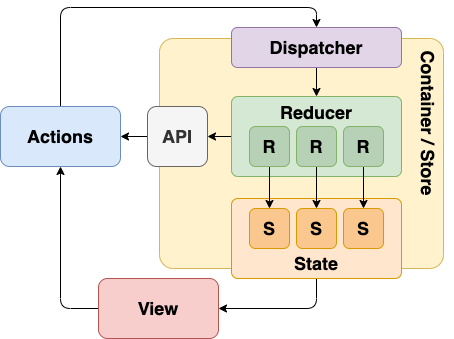
\includegraphics[width=\textwidth]{img/redux.png}
				\caption{Schema der Documenten-Scanner Architektur}
				\label{fig:redux}
			\end{subfigure}
			\begin{subfigure}[t]{0.48\textwidth}
				\centering
				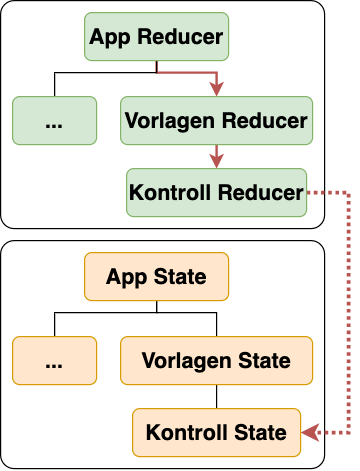
\includegraphics[height=0.9\textwidth]{img/tree_example.png}
				\caption{Reducer- und State-Objektbaum}
				\label{fig:tree}
			\end{subfigure}
			\caption{Architektur Schemata}
		\end{figure}
		
		Das Schema \ref{fig:redux} zeigt, die in der App umgesetzte Redux ähnliche Struktur. Über eine View (rot) können Aktionen (blau) aufgerufen werden. Diese gelangt zuerst in einen sogenannten Dispatcher (lila), welcher als Verteiler dient. Anhand der Art einer Aktion, wird der entsprechende Reducer (grün) vom Dispatcher beauftragt, die Aktion auszuführen. Ein Reducer ist für genau eine Art von Aktionen zuständig. Allerdings ist, wie in der \autoref{fig:tree} zu sehen ist, eine Schachtellung von Reducern (grün) möglich. Dies bedeutet auch, dass Aktions-Arten ineinander geschachtelt werden können. Das hat den Hintergrund, dass die States wie ein Objektbaum aufgebaut sind. So hat jeder State seinen eigenen Reducer, was für die oben erwähnte Modularität sorgt. Möchte man beispielsweise eine Änderung im Link State (siehe \ref{fig:tree}) vornehmen, muss die eigentliche Aktion in einer Link Reducer Aktion gekapselt werden und diese wiederum in einer Vorlagen Reducer Aktion. Zum ausführen der Aktion, werden dann die entsprechenden Reducer die Kapselung von außen nach innen auflösen. Nachdem die Aktion ausgeführt und eine State-Änderung herbeigeführt wurde, aktualisiert sich durch das data binding von MVVM die View. Genauer werden alle Views, die eine Bindung zu dem Datum haben, über die Änderung benachrichtigt und daraufhin aktualisieren diese sich.

		Ein weiterer wichtiger Punkt sind die Server-Aufrufe. Für diese gibt es einen eigenen Reducer und eine besondere Schnittstelle, welche in der \autoref{fig:redux} grau markiert und mit API \nomenclature{API}{application programming interface, deutsch: Programmierschnittstelle} beschriftet ist. Diese hat die Besonderheit selbst Aktionen an den Container zu senden. Beispielsweise löst ein Knopfdruck in einer View die Aktion aus, alle Vorlagen vom Server zu laden. Diese Aktion gelangt über den vorgesehenen Reducer zu der API-Schnittstelle. Dort wird ein entsprechender Server-Aufruf gestartet und ohne andere Prozesse anzuhalten auf den Server-Rückruf gewartet. Sobald die Antwort des Servers angekommen ist, wird diese in einer Aktion zurück zum Container gesendet. Dort wird sich wieder ein entsprechender Reducer um eventuelle Fehlerbehandlung oder das Ablegen der Vorlagen kümmern.
		
	\section{Implementierung}\label{sc:implementierung}
		
		Zur Realisierung der entworfenen Systemkomponenten wurde ausschließlich, die von Apple entwickelte IDE\nomenclature{IDE}{integrated development environment, deutsch: Integrierte Entwicklungsumgebung} Xcode\footurl{Xcode Internetseite -}{https://developer.apple.com/xcode/}, verwendet. Diese stellt Geräte-Simulatoren zur Verfügung, auf denen die App getestet werden kann. Die Simulatoren bieten unteranderem auch die Möglichkeit an, die Anwendung schnell auf verschiedenen iOS bzw. iPadOS Versionen zu testen. Auch ist das Testen der App auf echten Geräten durch Xcode möglich, was bei der Entwicklung unumgänglich war. Grund dafür ist die Benutzung der Kamera, die bei den Simulatoren zu gewollten Abstürzen führt, da diese keinen Zugriff auf eine Kamerasystem besitzen.
		
		Die App wurde ausschließlich in der Programmiersprache Swift geschrieben. Zusätzlich wurden die Frameworks SwiftUI, Vision und VisionKit von Apple, sowie das Framework Kingfisher\footurl{Kingfisher GitHub Repository -}{https://github.com/onevcat/Kingfisher}, zum Downloaden und Cachen von Bildern verwendet. Das Vision-Framework führt Erkennung von Gesichts- und Gesichtsmarkierungen, Texterkennung, Barcode-Erkennung, Bildregistrierung und allgemeine Merkmalsverfolgung durch. Jedoch wurde in der App nur die integrierte Texterkennung benutzt. Es ist aber anzunehmen, das Algorithmen aus VisionKit von Vision zur Dokumenten-Erkennung verwendet. Für mehr Informationen über die Frameworks SwiftUI und VisionKit siehe im \autoref{ch:prototyp} \autoref{sc:analyse}.
		
		Zum Ändern und Testen des Backends wurde außerdem Visual Studio Community bzw. Visual Studio Code\footurl{Visual Studio Internetseite -}{https://visualstudio.microsoft.com/de/} mit dem REST Client Plugin\footurl{REST Client, ein Visual Studio Code Plugin -}{https://marketplace.visualstudio.com/items?itemName=humao.rest-client} , zum Testen der Server-Schnittstellen verwendet. Das Backend konnte dann als lokaler Server auf dem Entwicklungscomputer gestartet und über die IP-Adresse 0.0.0.0 sogar im lokalen Netzwerk aufgerufen werden. Für die Verwaltung der PostgreSQL-Datenbank genügte das Tool PgAdmin4\footurl{PgAdmin Internetseite -}{https://www.pgadmin.org/}. Damit ist es möglich einzelne Einträge oder auch ganze Tabellen der Datenbank zu bearbeiten.
		
		\begin{figure}[th]
    		\centering
   			\begin{subfigure}[t]{0.3\textwidth}
       			\frame{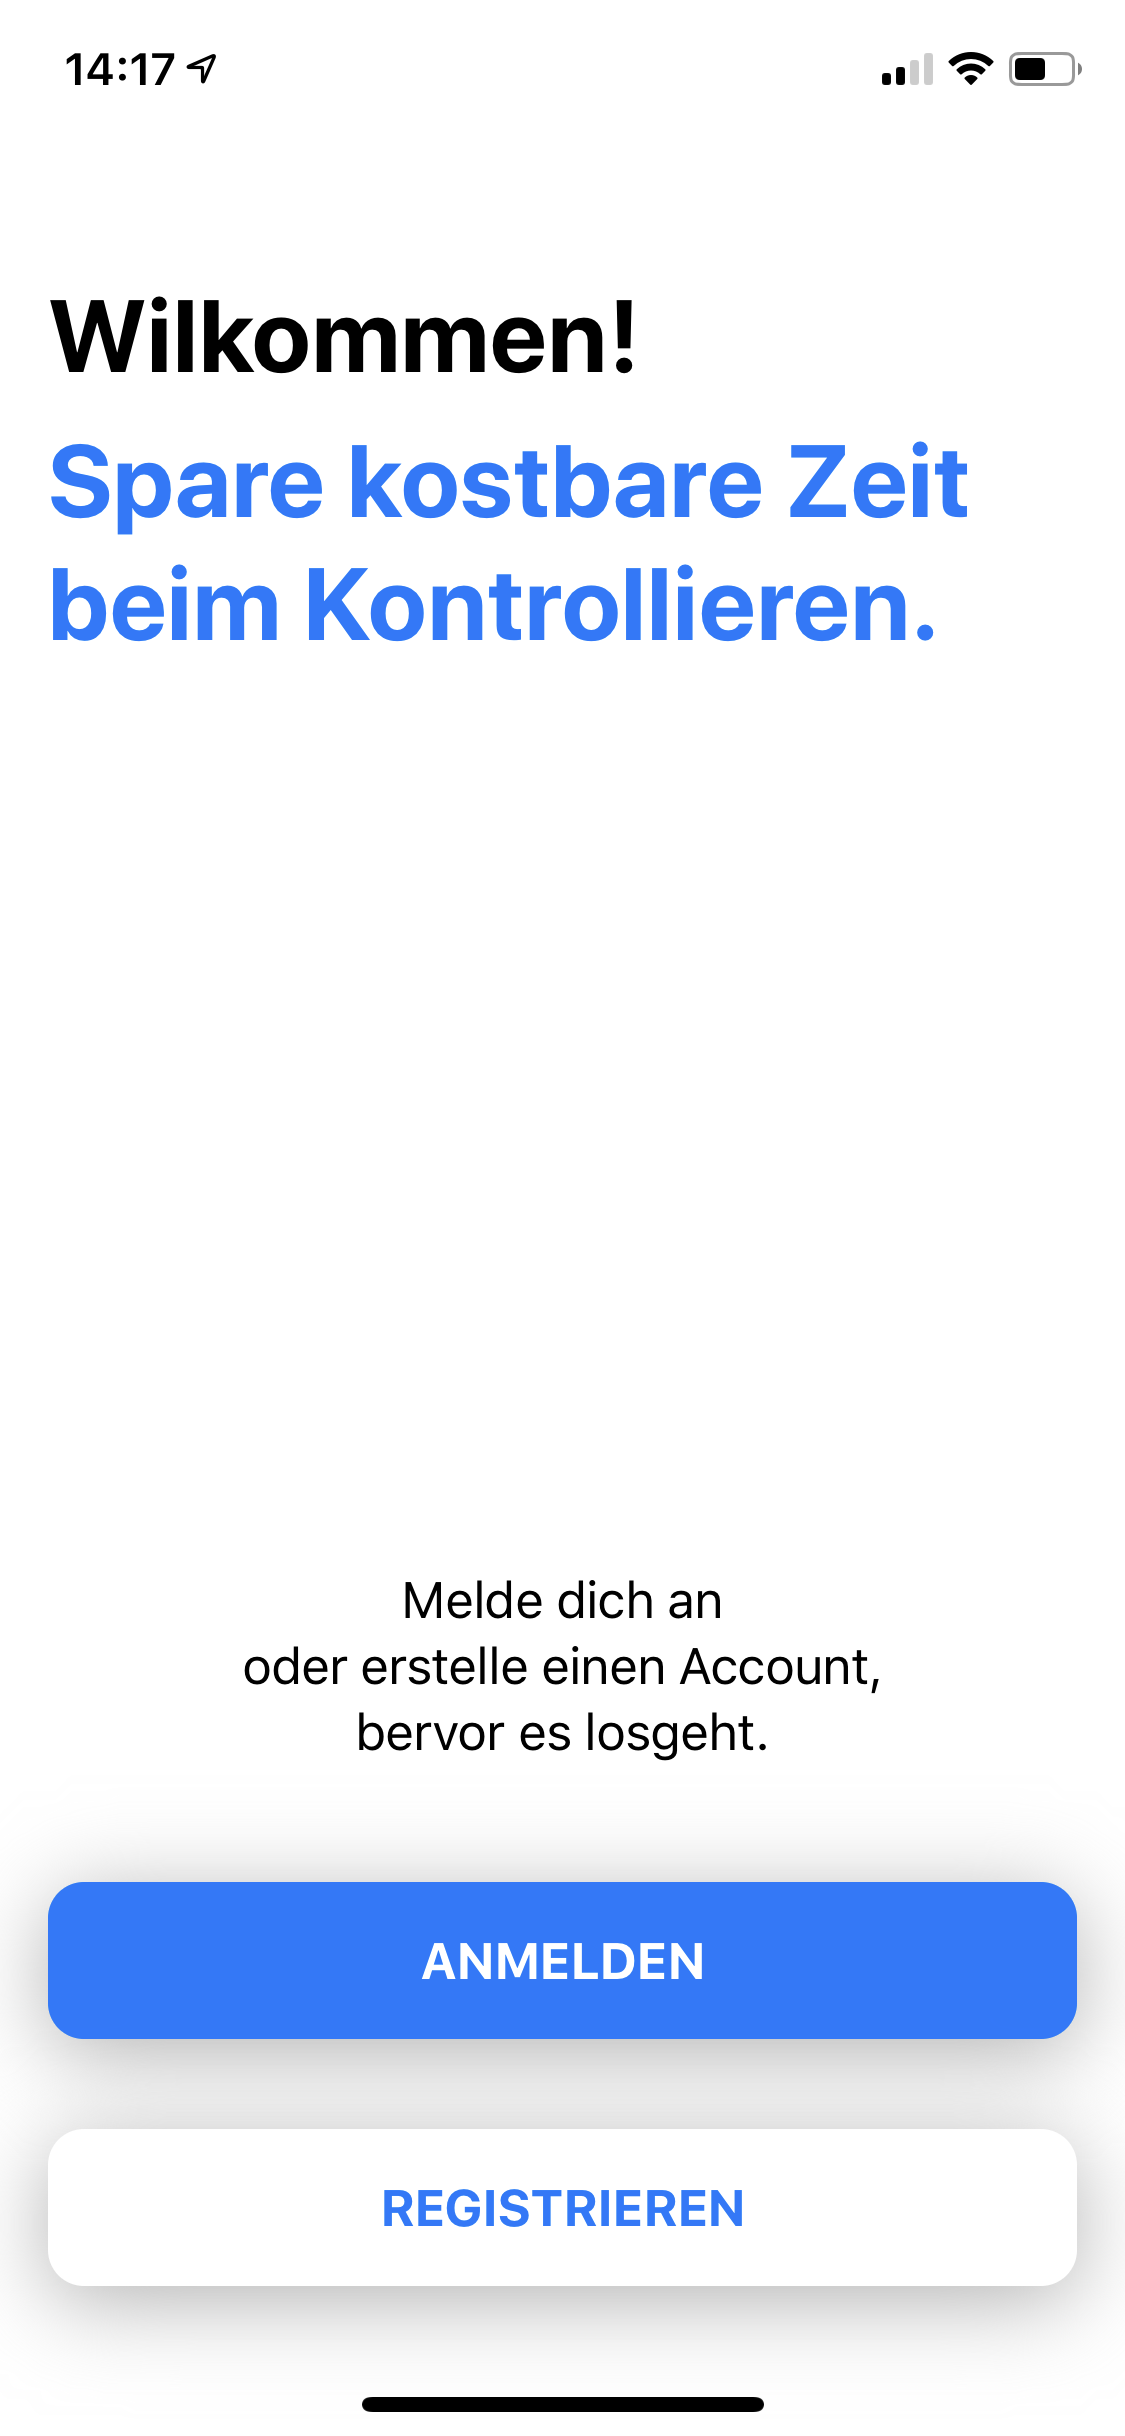
\includegraphics[width=0.96\textwidth]{img/1willkommen.png}}
       			\caption{Willkommen View}
       			\label{fig:willkommen}
       		\end{subfigure}
    		\begin{subfigure}[t]{0.3\textwidth}
        		\frame{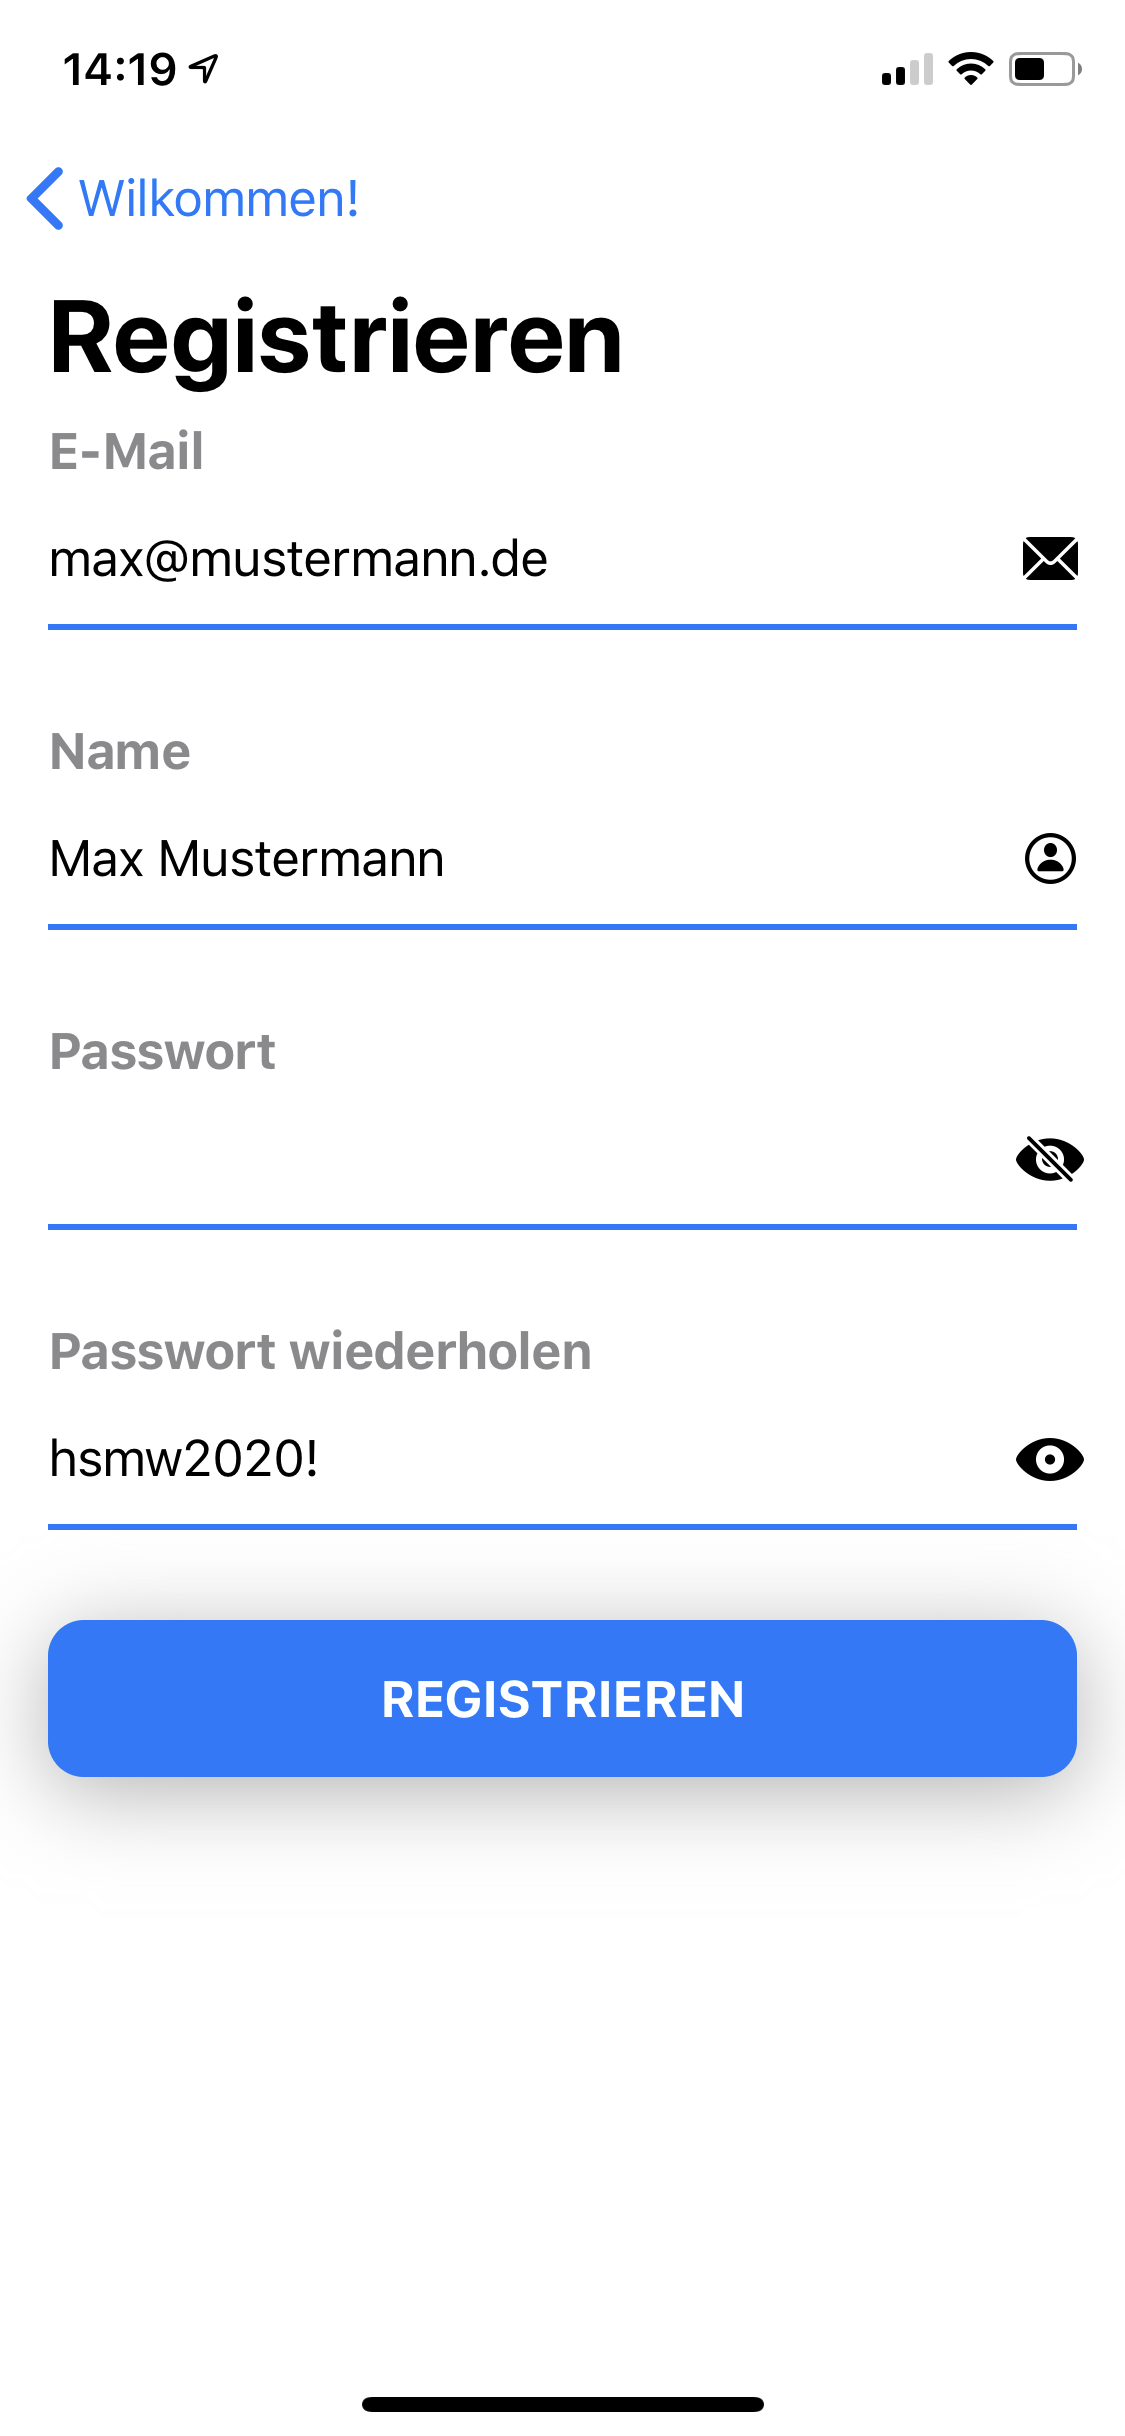
\includegraphics[width=0.96\textwidth]{img/7reg_full_see.png}}
      			\caption{Registrierung mit sicheren Eingabefeldern}
       			\label{fig:register}
   			\end{subfigure}
   			\begin{subfigure}[t]{0.3\textwidth}
      			\frame{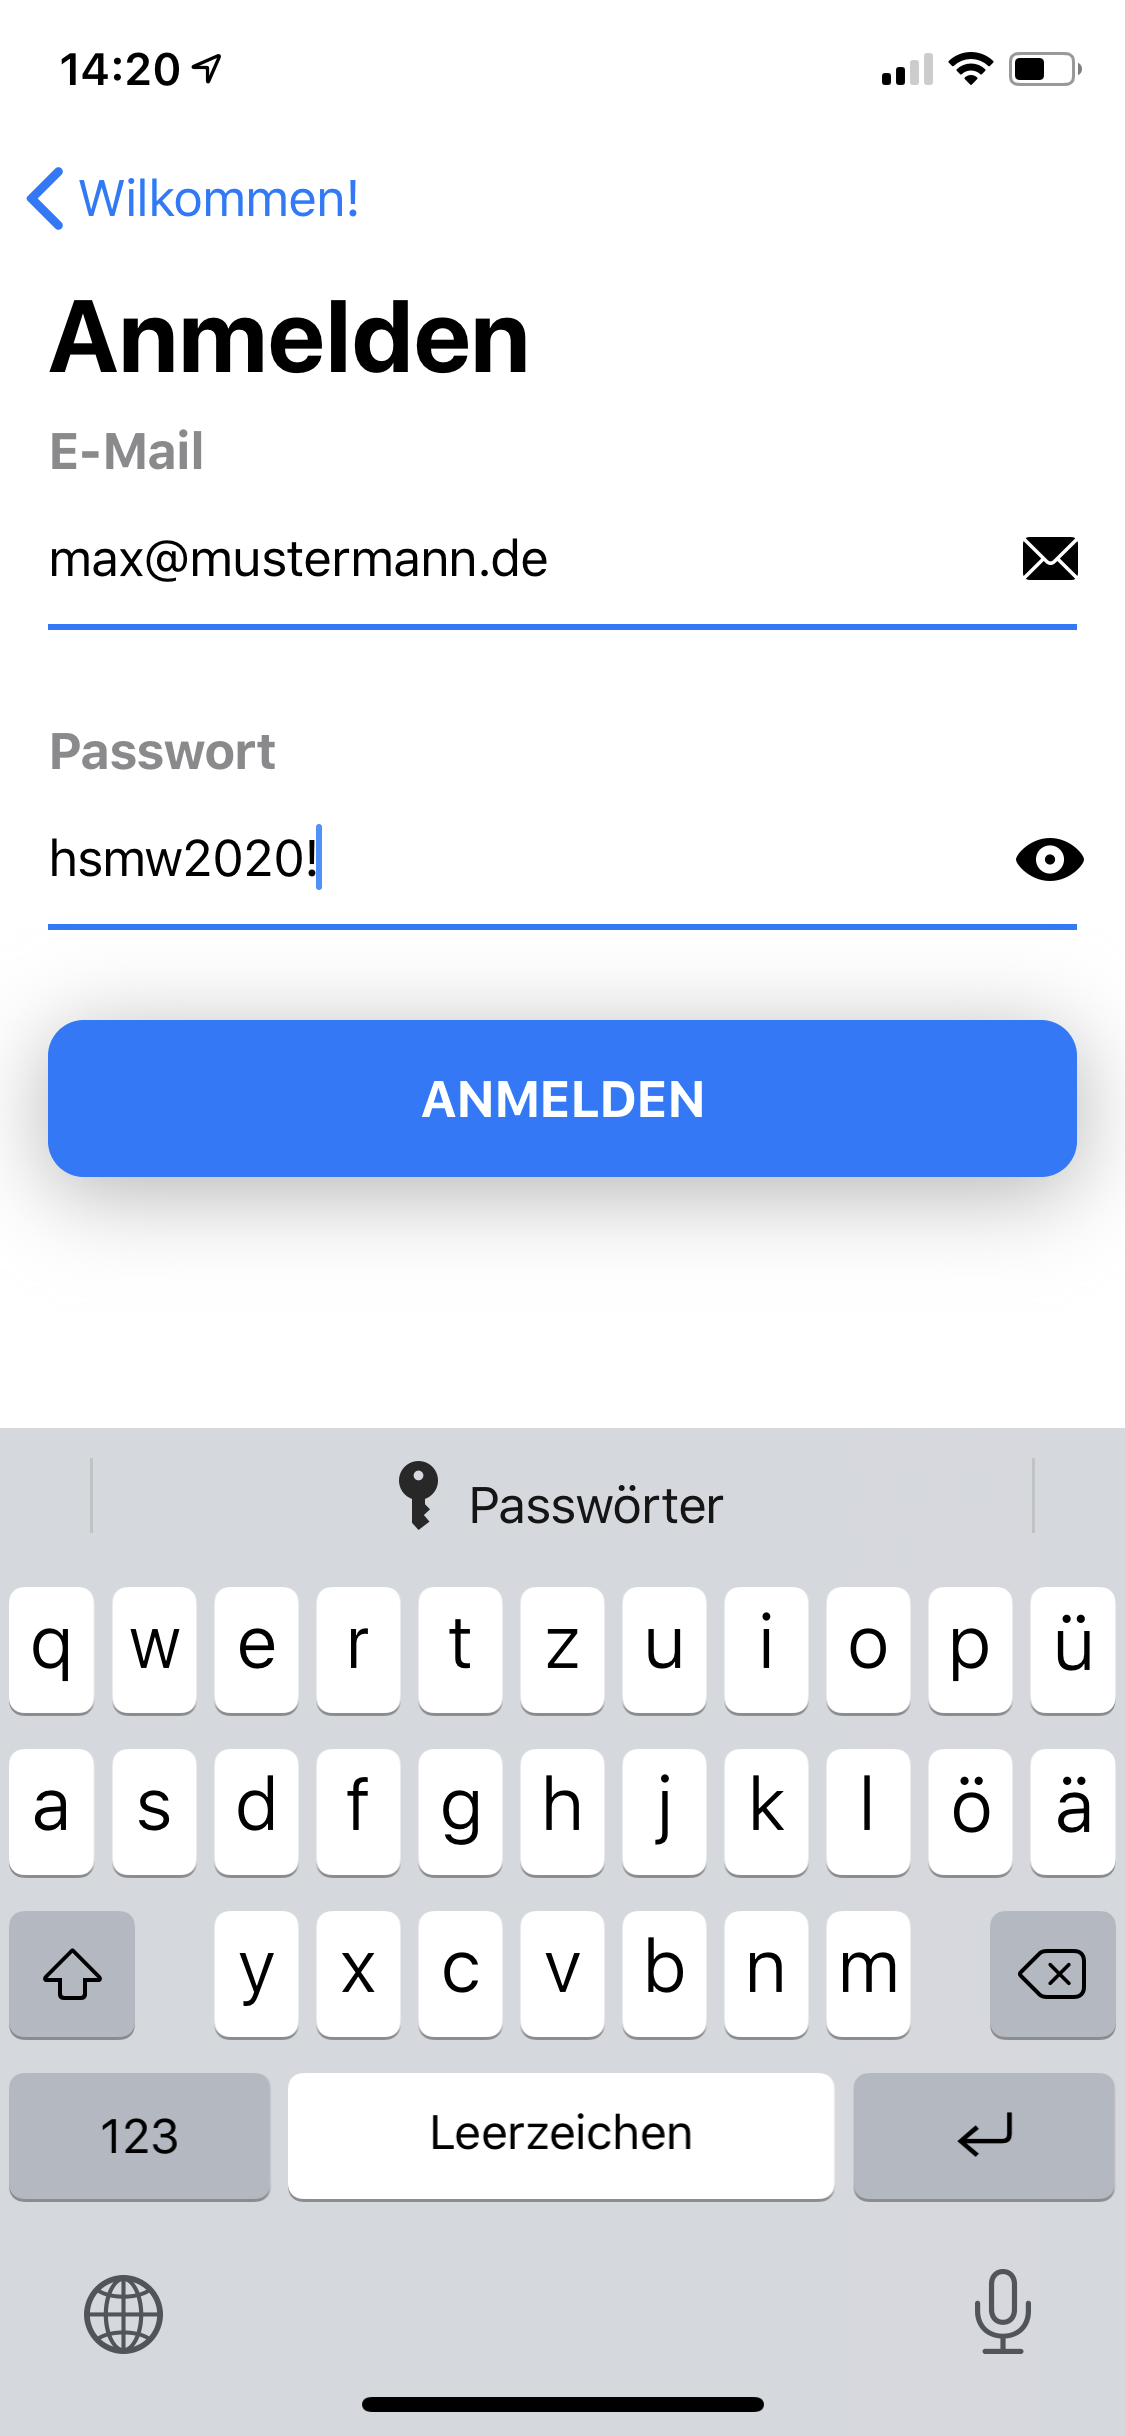
\includegraphics[width=0.96\textwidth]{img/12an_full_pass.png}}
        		\caption{Anmeldung mit AutoFill-Funktion}
	       		\label{fig:anmelden}
    		\end{subfigure}
   			\caption{Willkommen- Registrier- und Anmelde-View}\label{fig:start}
		\end{figure}
		
		\subsection{Registrieren und Anmelden}
			Die technische Implementierung der Registrierung und Anmeldung beinhaltet typische Charakteristiken von Anmelde- und Registrier-Formularen. Die E-Mail-Textfelder besitzen, wie auch das Passwort-Feld der Anmeldung eine AutoFill-Funktion. Dadurch kann das iOS-Gerät Registrier- und Anmelde-Daten vorschlagen und automatisch in die entsprechenden Felder einsetzten. Dies sieht man im dritten Bild \ref{fig:anmelden} anhand des ''Passwörter''-Knopfes über der Tastatur.  Weiter sind alle Passwort-Felder gesichert. Das bedeutet, dass der Inhalt zum Schutz der Privatsphäre standardmäßig ausgeblendet und mit Punkten ersetzt wird. Durch das drücken des Auges rechts des Textfeldes kann der Inhalt jedoch eingesehen werden. Im mittlerem Bild \ref{fig:register} sind wegen der Sicherheitsstandards von iOS, bei einer Aufnahme des Bildschirms nicht einmal die Ersatz-Punkte des ersten Passwort-Textfelds zu sehen. Zusätzlich validieren alle Text-Felder ihren Inhalt mithilfe von regulären Ausdrücken. Beispielsweiße muss ein Passwort aus 8 Zeichen bestehen und zwei von den drei Folgenden Eigenschaften erfüllen:
			\begin{enumerate}
				\item Es ist mindestens ein Sonderzeichen enthalten.
				\item Es ist mindestens ein Großbuchstabe enthalten.
				\item Es ist mindestens eine Zahl enthalten.
			\end{enumerate}
			Die Validierung ist jedoch nicht standardmäßig, sondern wurde selbst entwickelt.
			
		\subsection{Scan-Vorlagen erstellen und speichern}
			Bei der Implementierung des ersten Arbeitsschritts der Scan-Vorlagen wurde das schriftliche Flussdiagramm, welches im Anhang \ref{ch:workflow} zu finden ist, leicht verändert benutzt.
			
			\subsubsection*{Scan-Vorlage erstellen}
			\begin{figure}[th]
    			\centering
    			\begin{subfigure}[t]{0.3\textwidth}
        			\frame{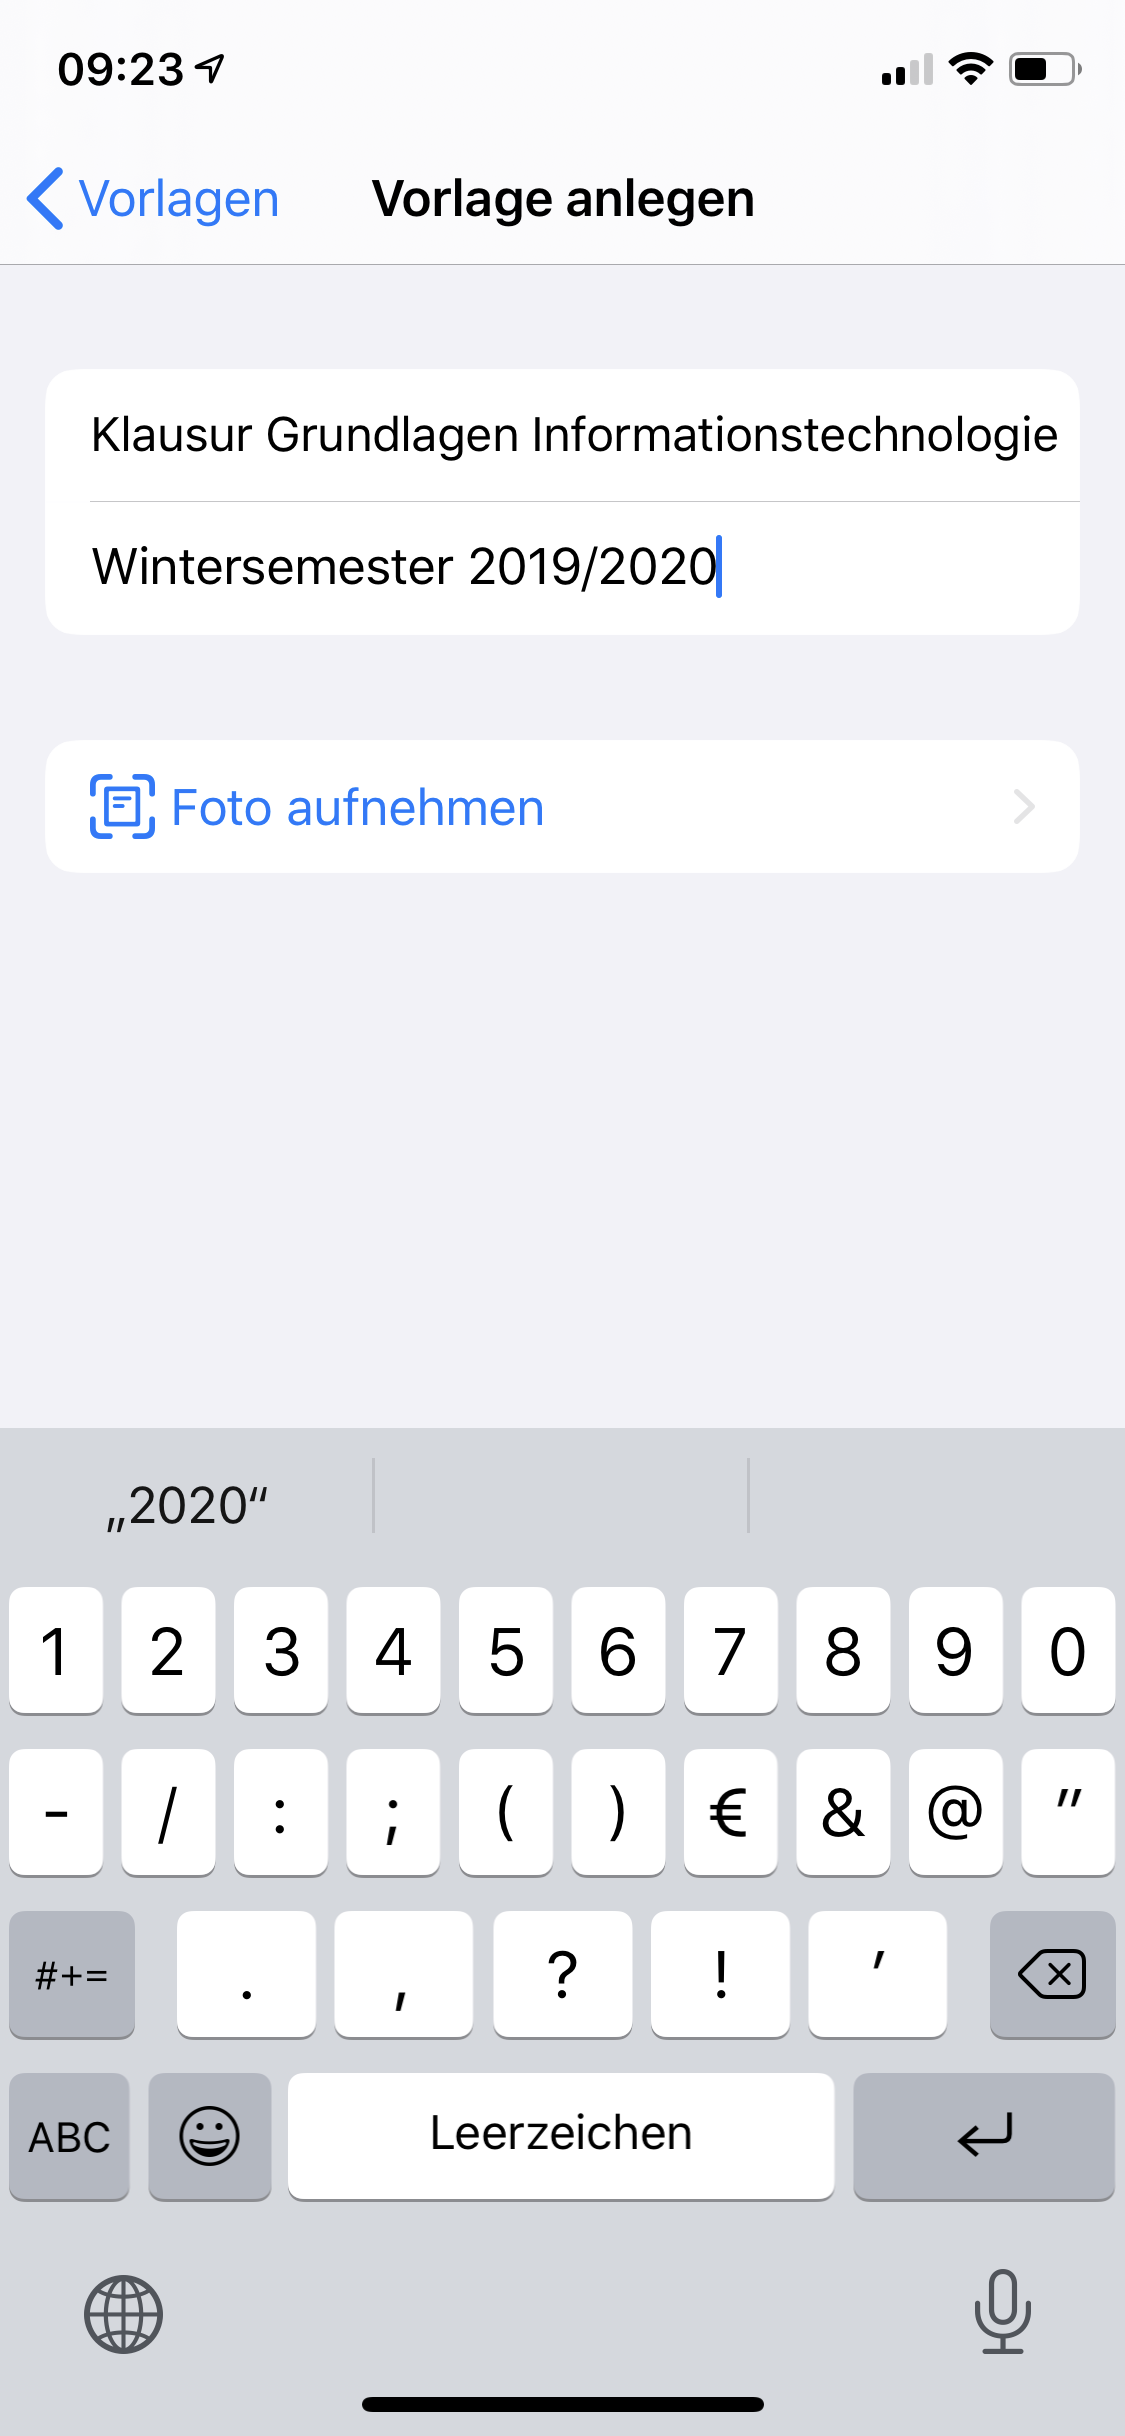
\includegraphics[width=0.96\textwidth]{img/V2}}
        			\caption{View zum Anlegen einer Vorlage}
        			\label{fig:v2}
    			\end{subfigure}
    			\begin{subfigure}[t]{0.3\textwidth}
        			\frame{\includegraphics[width=0.96\textwidth]{img/V3}}
        			\caption{Kamera- Scan-View mit Dokumenten-Erkennung}
        			\label{fig:v3}
    			\end{subfigure}
    			\begin{subfigure}[t]{0.3\textwidth}
       				\frame{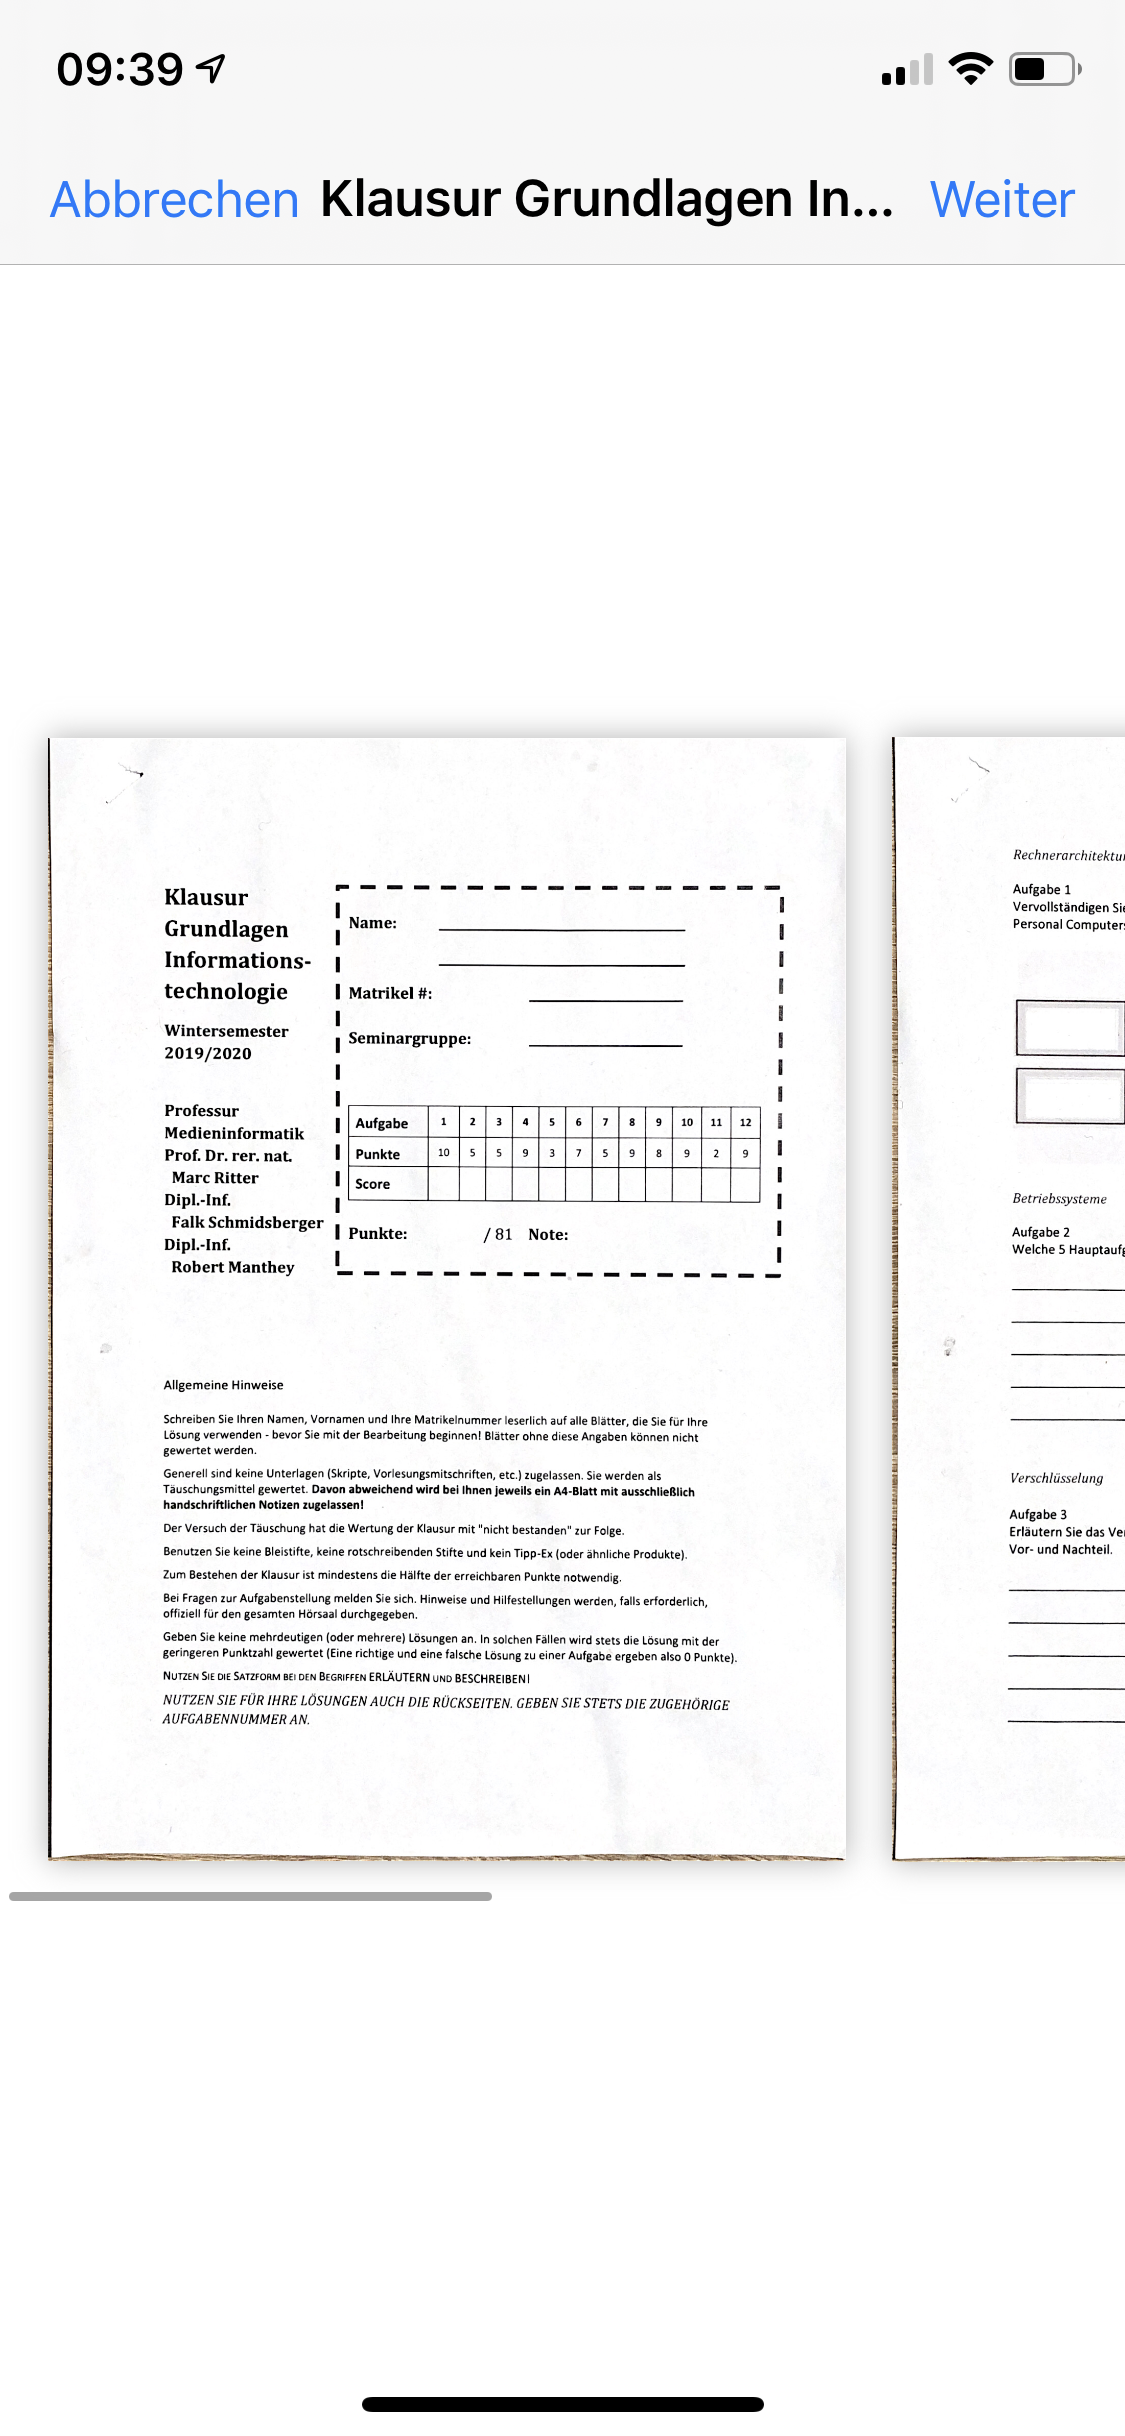
\includegraphics[width=0.96\textwidth]{img/V4}}
        			\caption{Seiten-Auswahl-View}
        			\label{fig:v4}
    			\end{subfigure}
    			\caption{Die ersten Views zur Erstellung einer Scan-Vorlage}\label{fig:erstellung1}
			\end{figure}
			
			Im ersten Schritt sind ein Name und weitere Informationen, zu der Vorlage an zugegeben (siehe \ref{fig:v2}), um im Anschluss die Fotos aufzunehmen. Bei der Kamera-View (siehe \ref{fig:v3}) handelt es sich um die Scan-View des Frameworks VisionKit. Mithilfe von Kantenerkennung und anderen Algorithmen, die Tobias Kallauke in seinem Bericht beschreibt, kann dass Dokument sobald es erkannt ist, automatisch fotografiert werden. In Echtzeit wird das erkannte Dokument aus dem Bild ausgeschnitten und gerade gezogen. Ein manuelles Auslösen des Fotos und Anpassen der Dokumenten-Kanten im Bild, ist ebenfalls möglich. Des Weiterem werden alle erstellten Bilder zu einer Gruppe gesammelt. Diese können vor dem Abspeichern angeschaut und nochmal bearbeitet werden. Die \autoref{fig:klausur} entstand durch diesen Prozess.
			
			\subsubsection*{Regionen erstellen}
			\begin{figure}[th]
    			\centering
    			\begin{subfigure}[t]{0.3\textwidth}
        			\frame{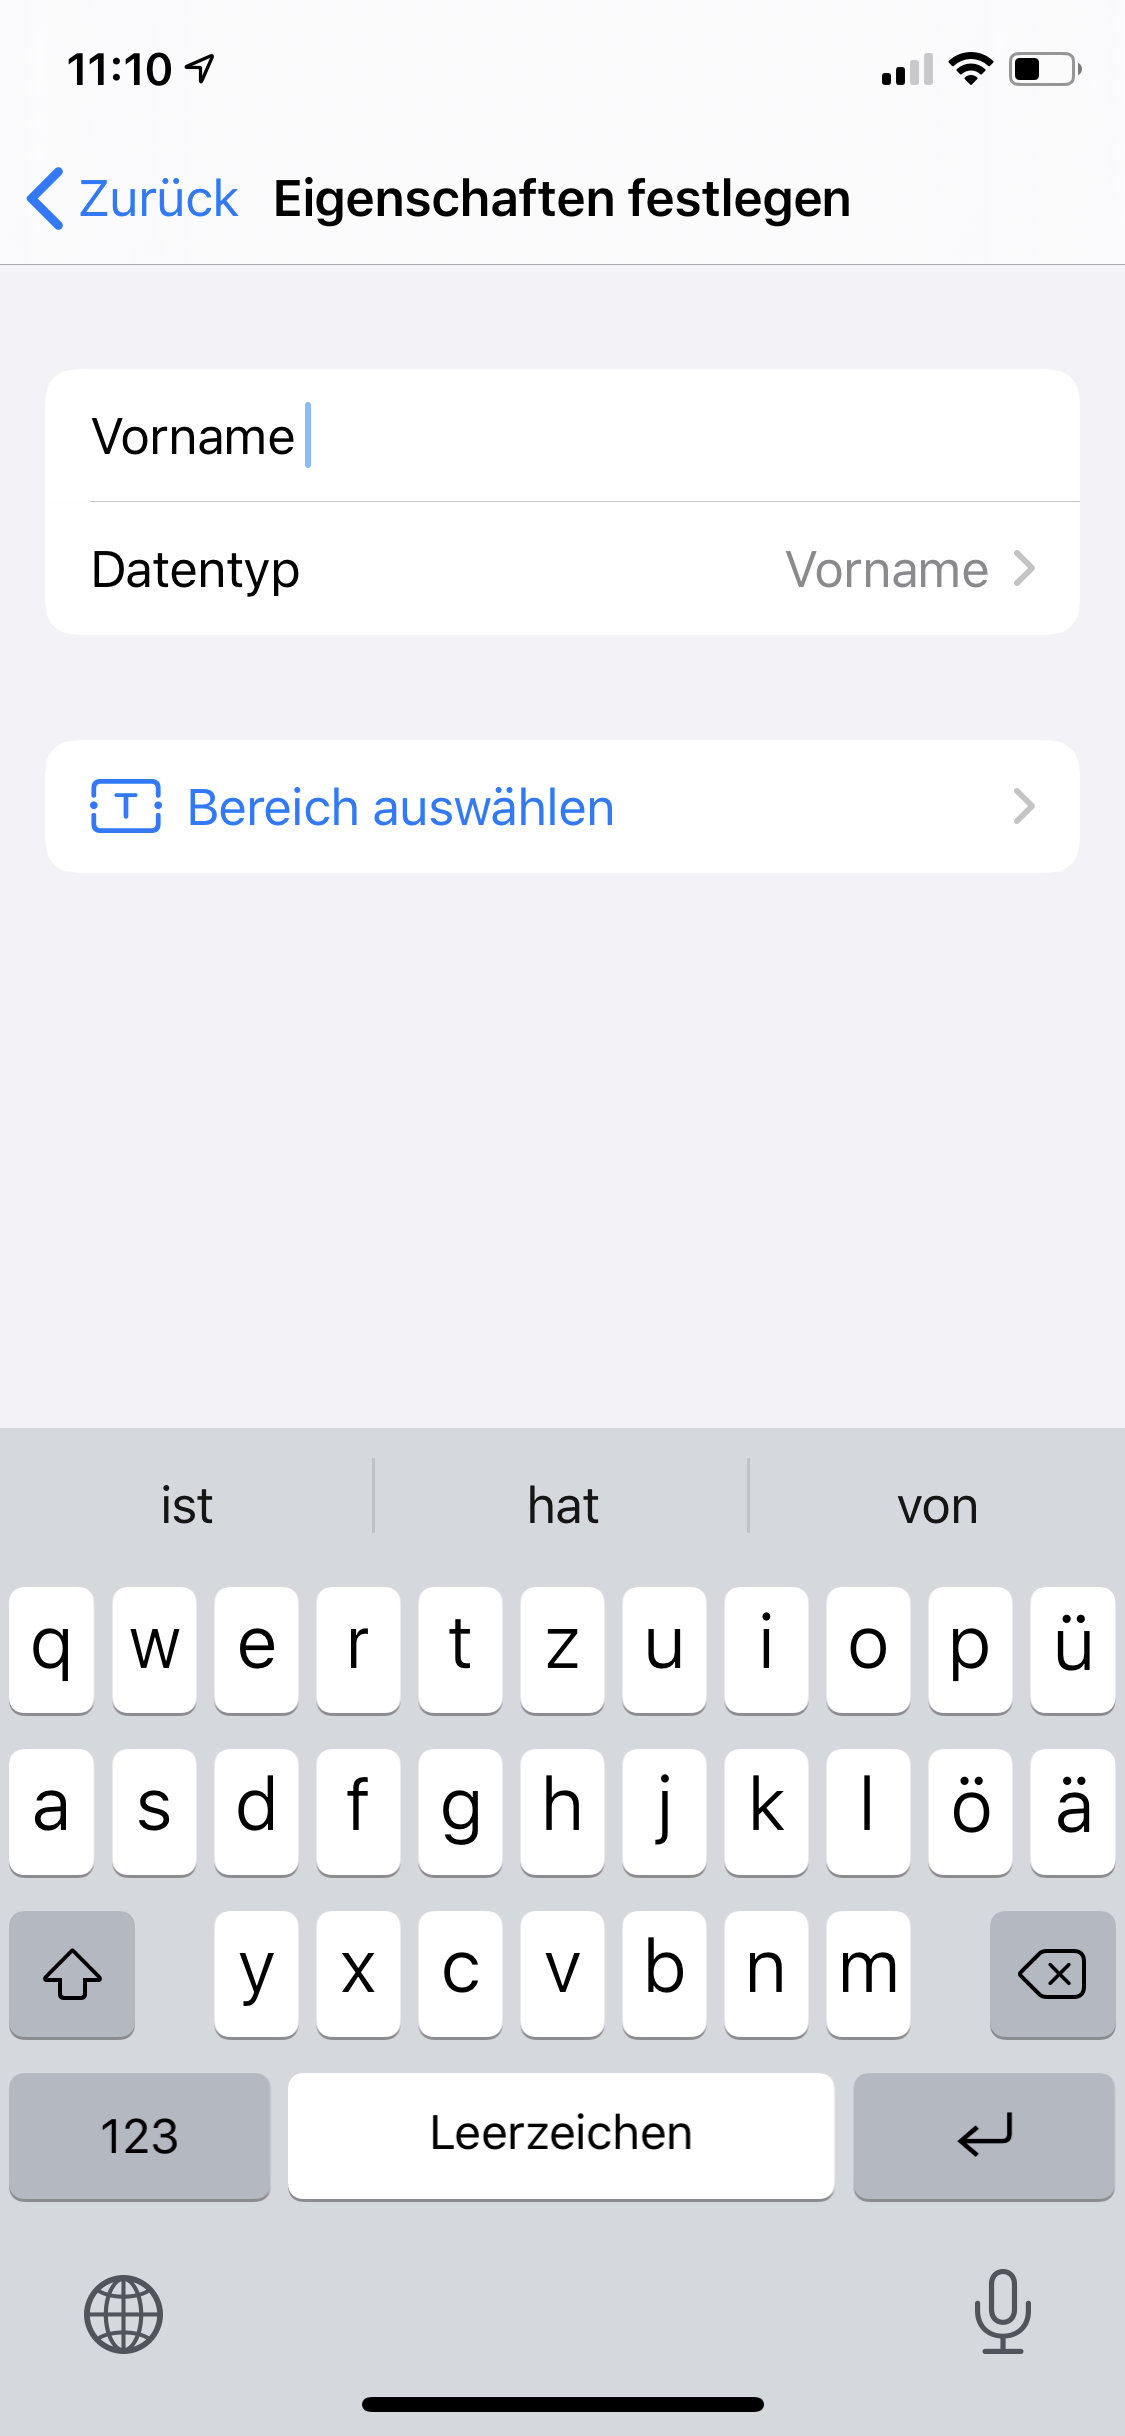
\includegraphics[width=0.96\textwidth]{img/V5}}
        			\caption{View zum Festlegen von den Regionen Eigenschaften}
        			\label{fig:v5}
    			\end{subfigure}
    			\begin{subfigure}[t]{0.3\textwidth}
        			\frame{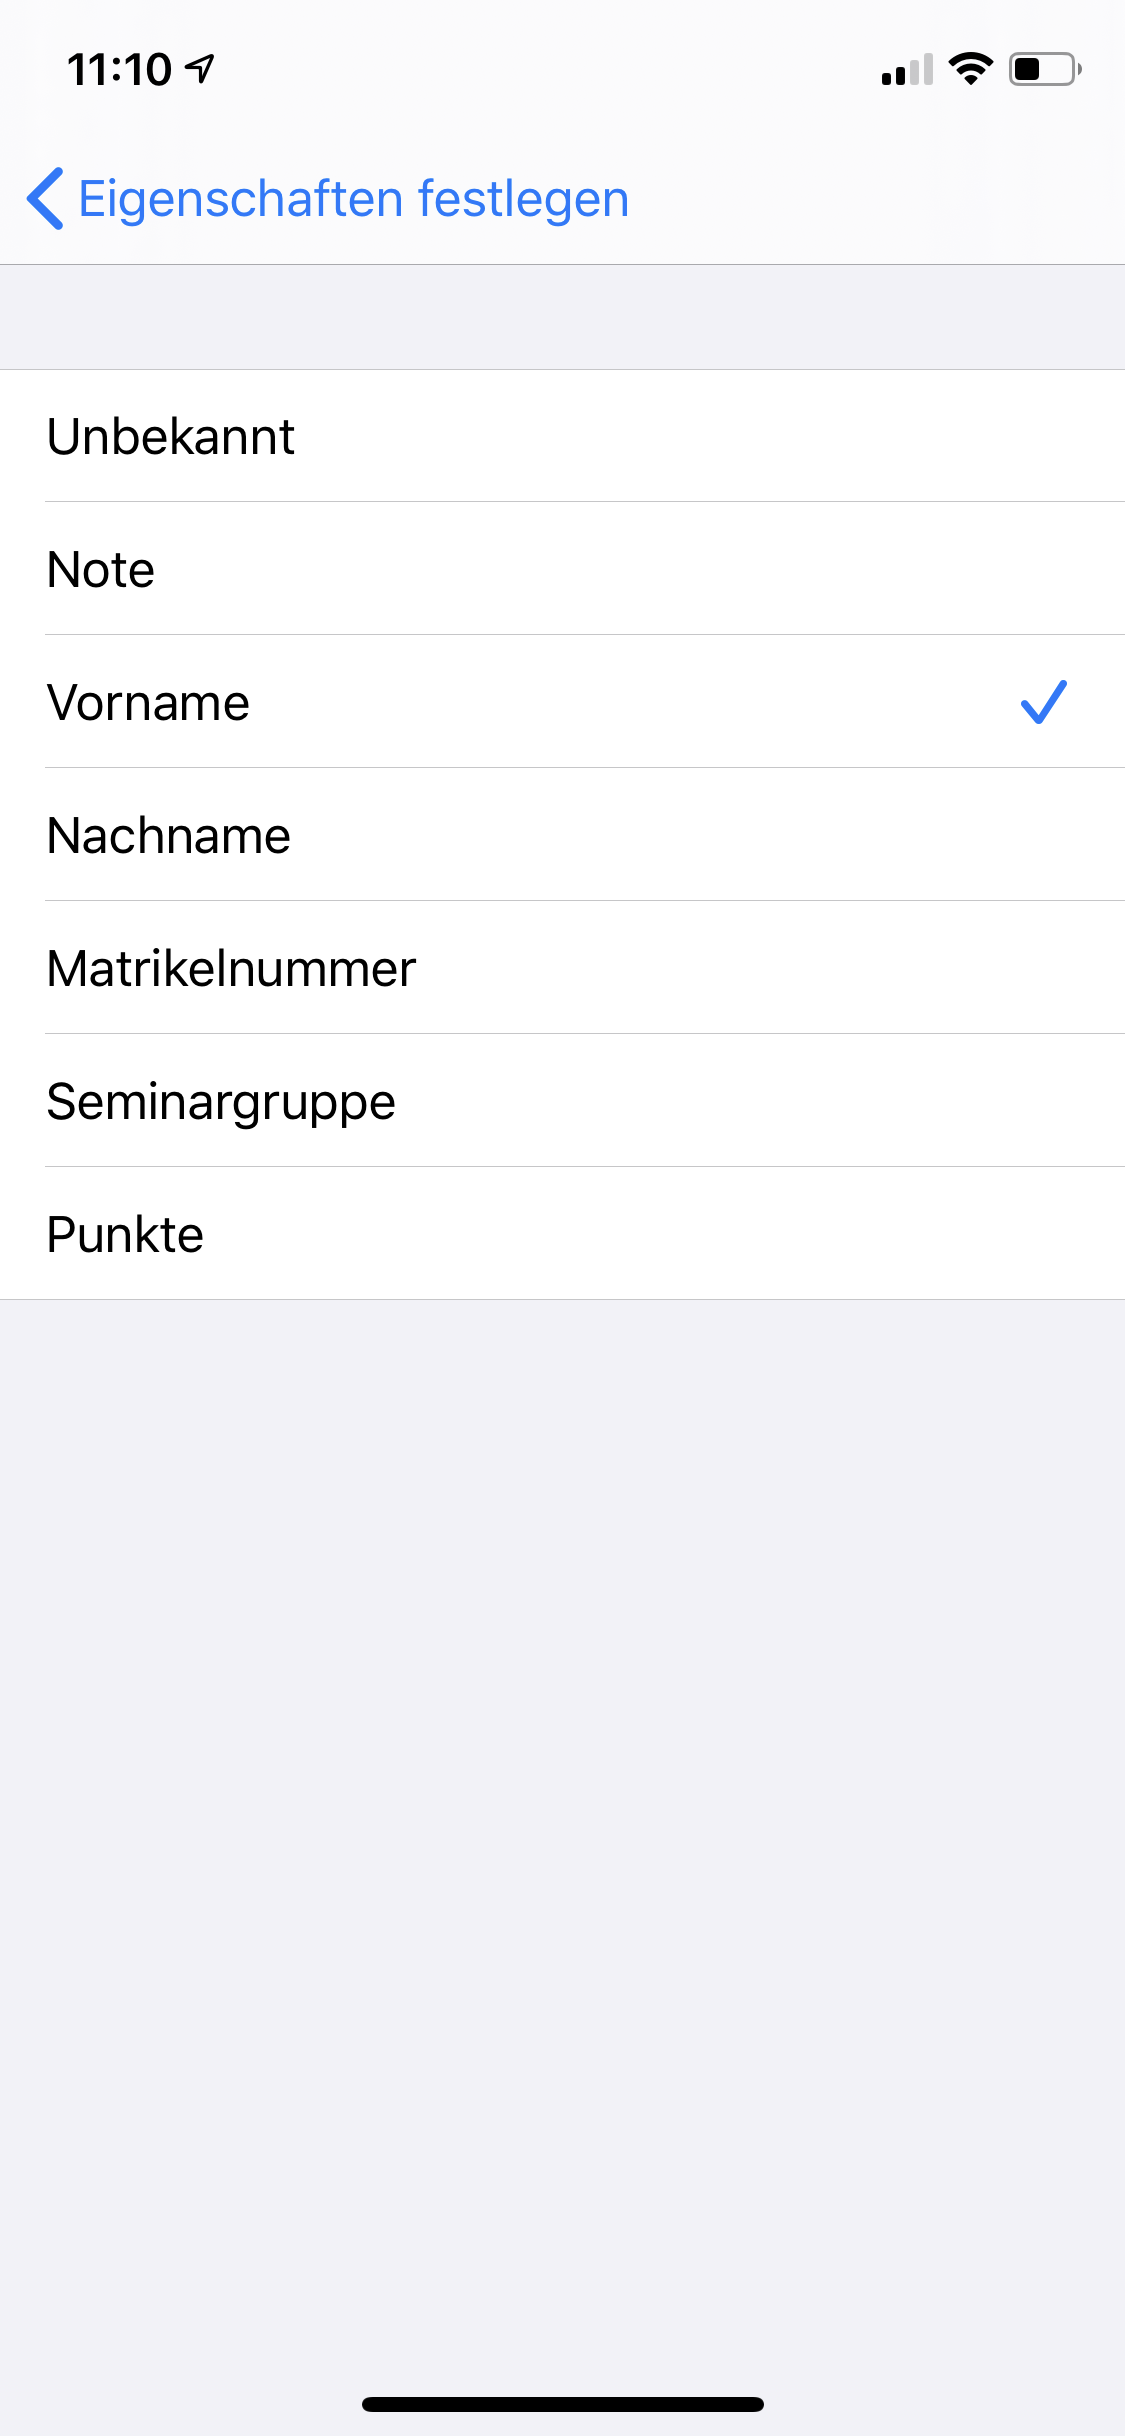
\includegraphics[width=0.96\textwidth]{img/V6}}
        			\caption{Auswahl des Datentyps}
        			\label{fig:v6}
    			\end{subfigure}
    			\begin{subfigure}[t]{0.3\textwidth}
       				\frame{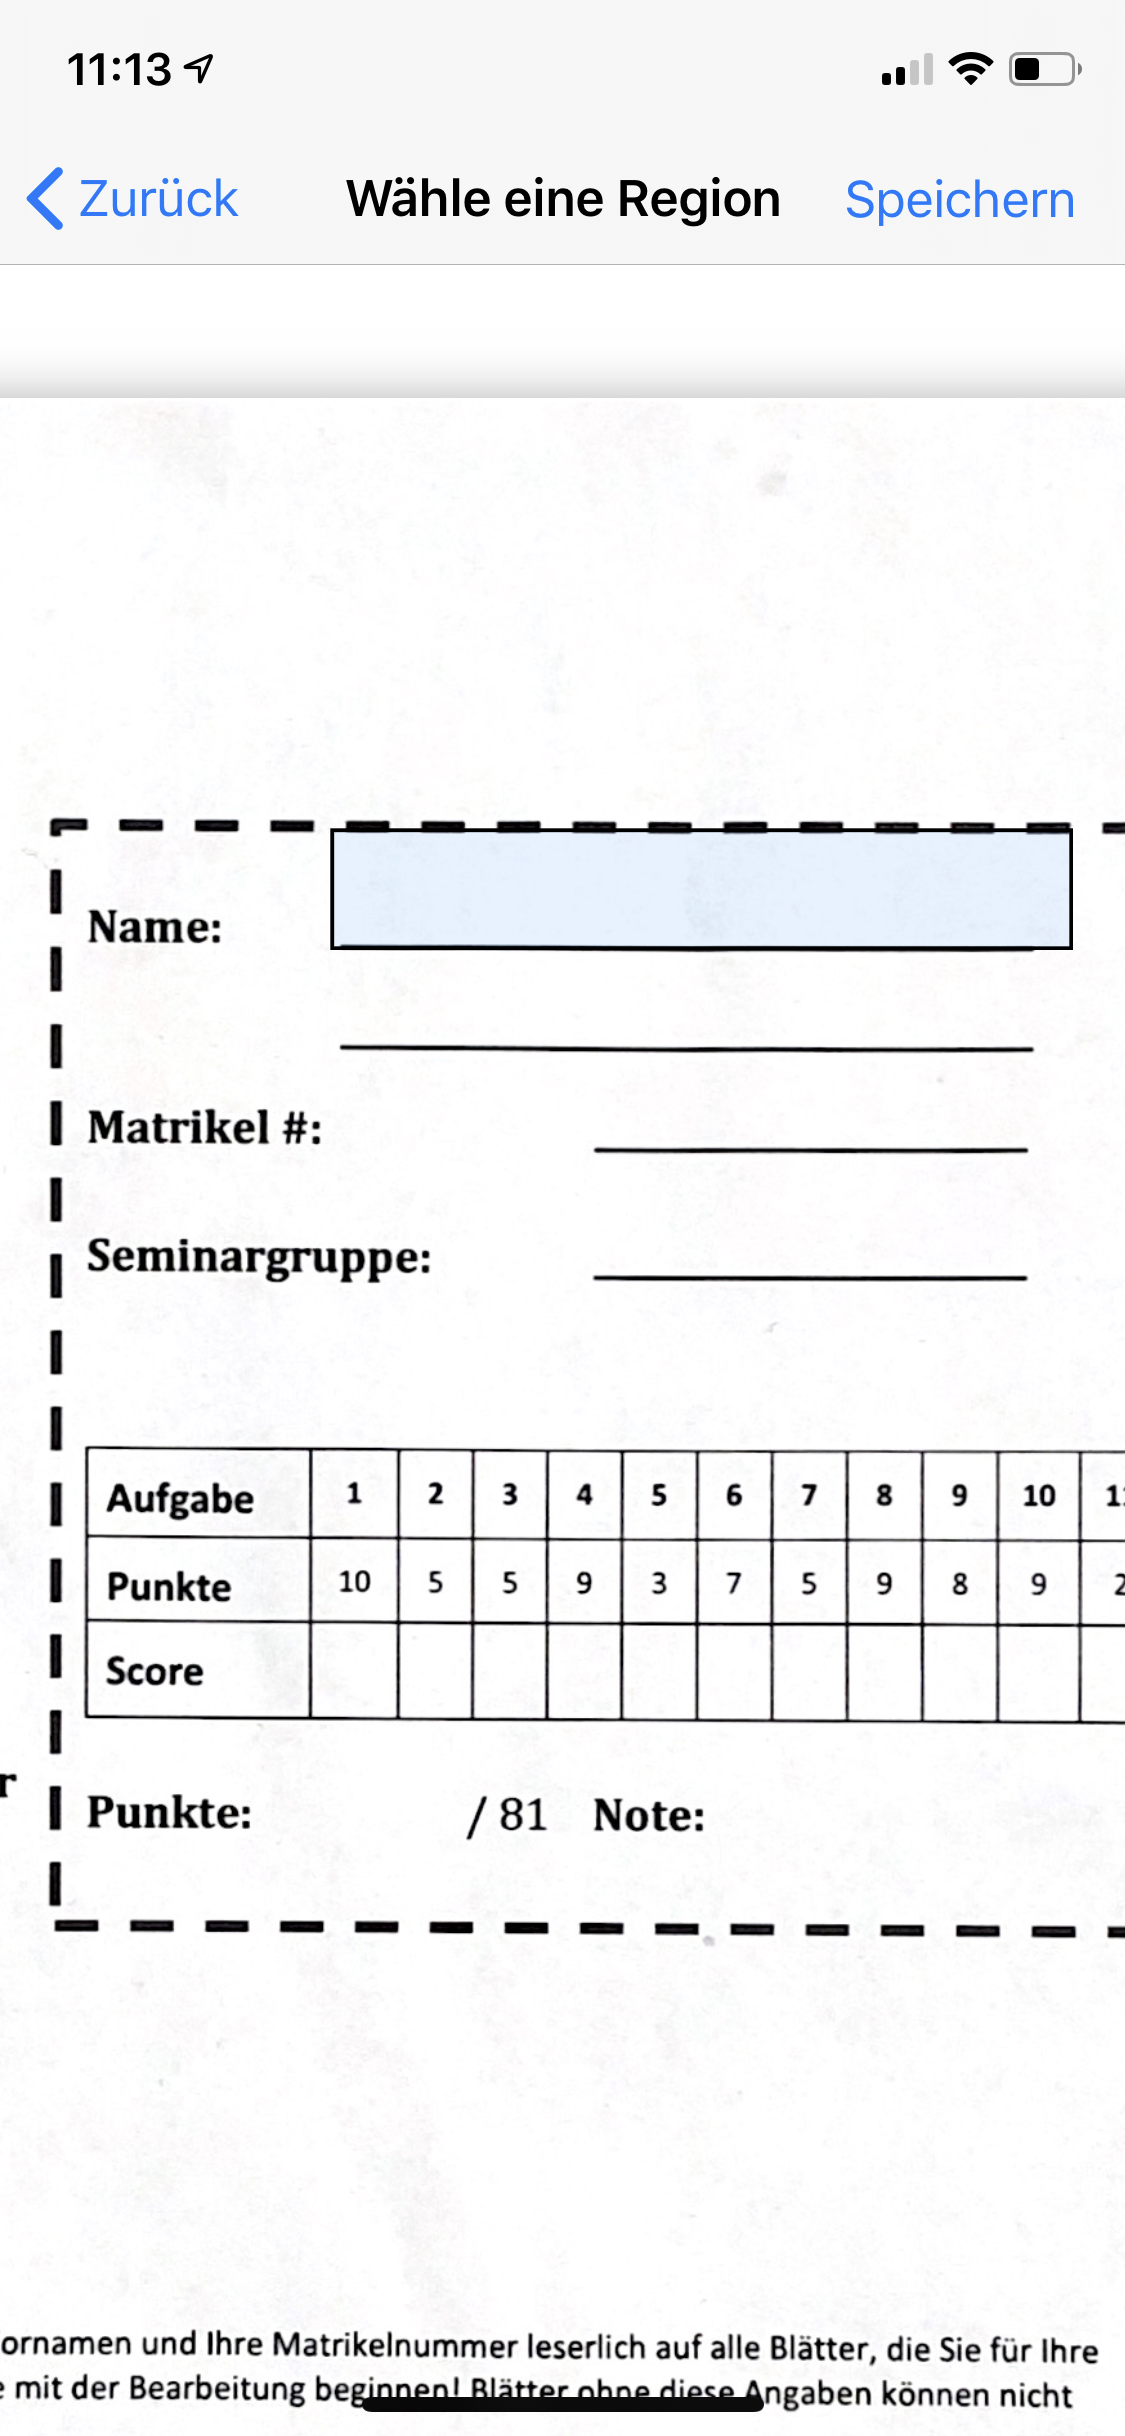
\includegraphics[width=0.96\textwidth]{img/V7}}
        			\caption{Markierung der Region auf dem Dokument}
        			\label{fig:v7}
    			\end{subfigure}
    			\caption{Views zur Erstellung von Regionen}
    			\label{fig:erstellung2}
			\end{figure}
			
			\begin{figure}[th]
    			\centering
				\begin{subfigure}[t]{0.3\textwidth}
       				\frame{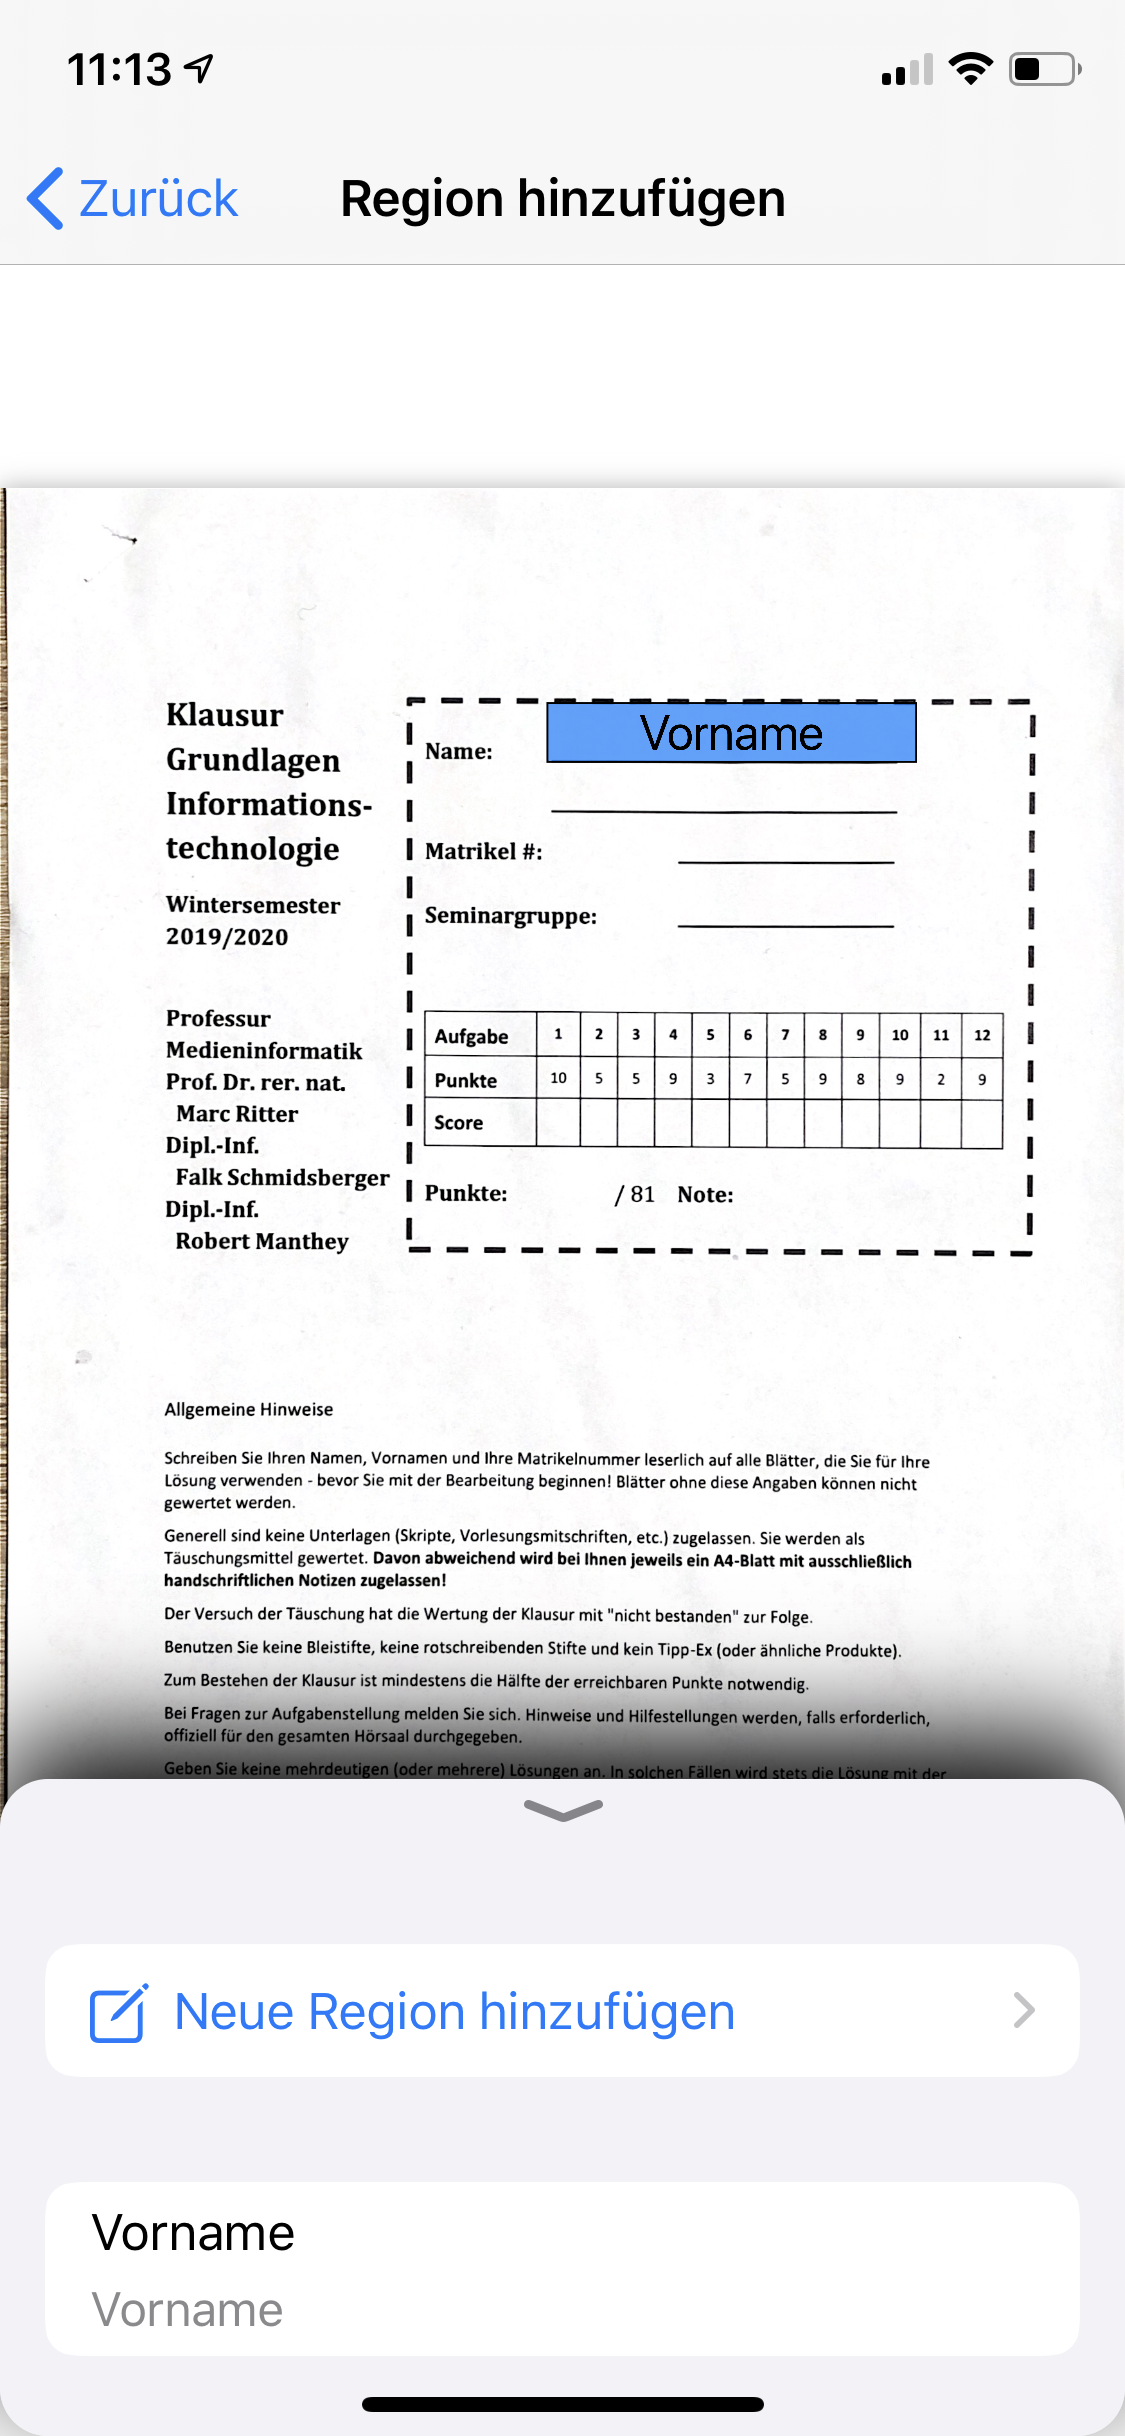
\includegraphics[width=0.96\textwidth]{img/V8}}
        			\caption{Seiten-Vorschau mit der ersten Region}
        			\label{fig:v8}
    			\end{subfigure}
    			\begin{subfigure}[t]{0.3\textwidth}
       				\frame{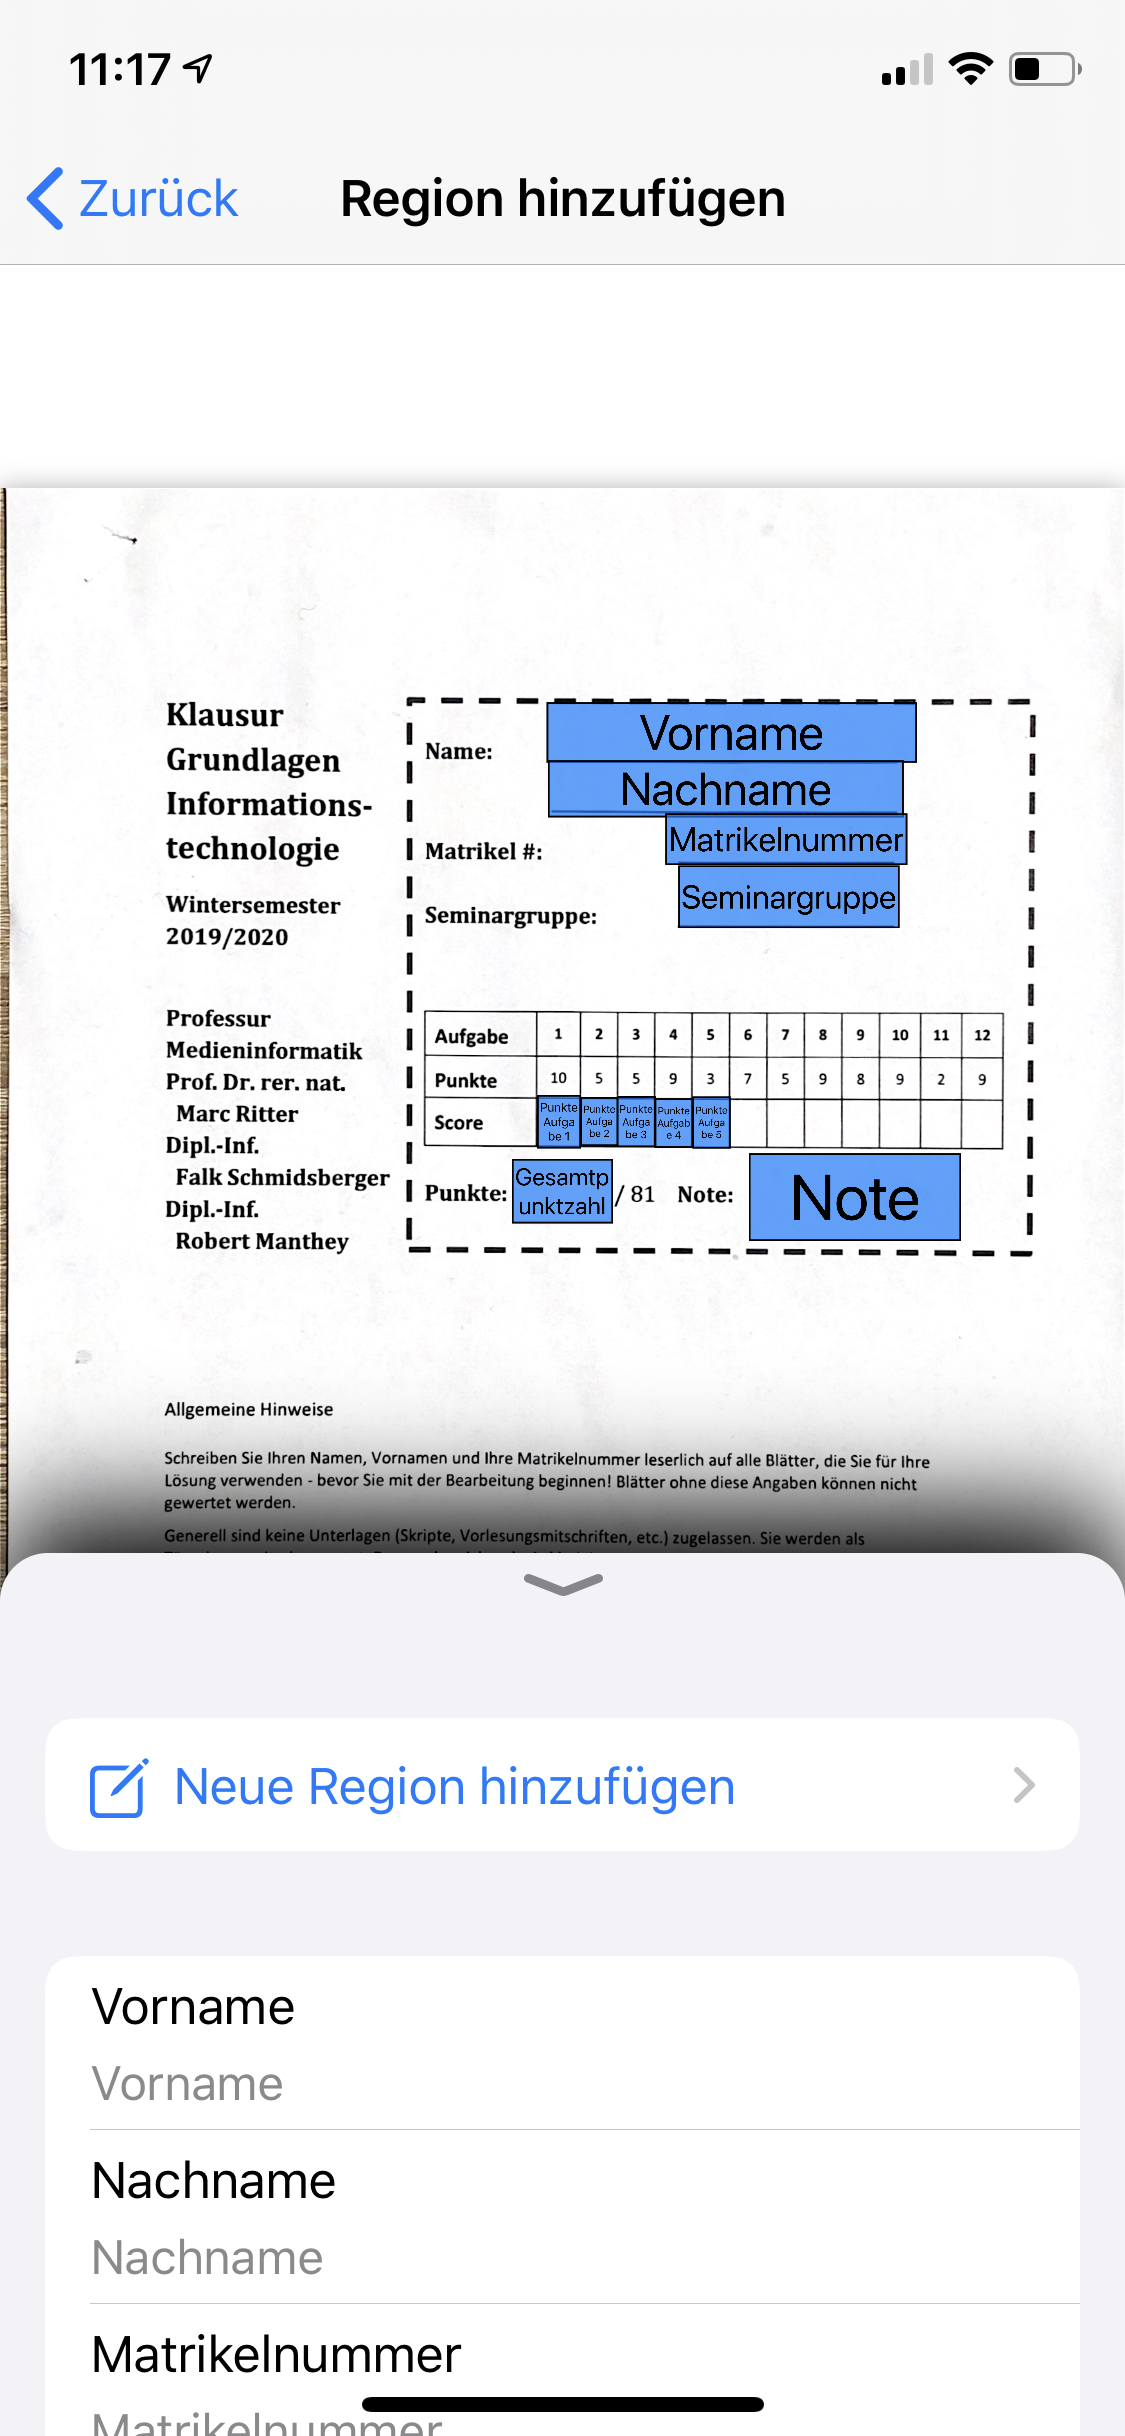
\includegraphics[width=0.96\textwidth]{img/V9}}
        			\caption{Seiten-Vorschau mit allen Regionen}
        			\label{fig:v9}
    			\end{subfigure}
    			\begin{subfigure}[t]{0.3\textwidth}
       				\frame{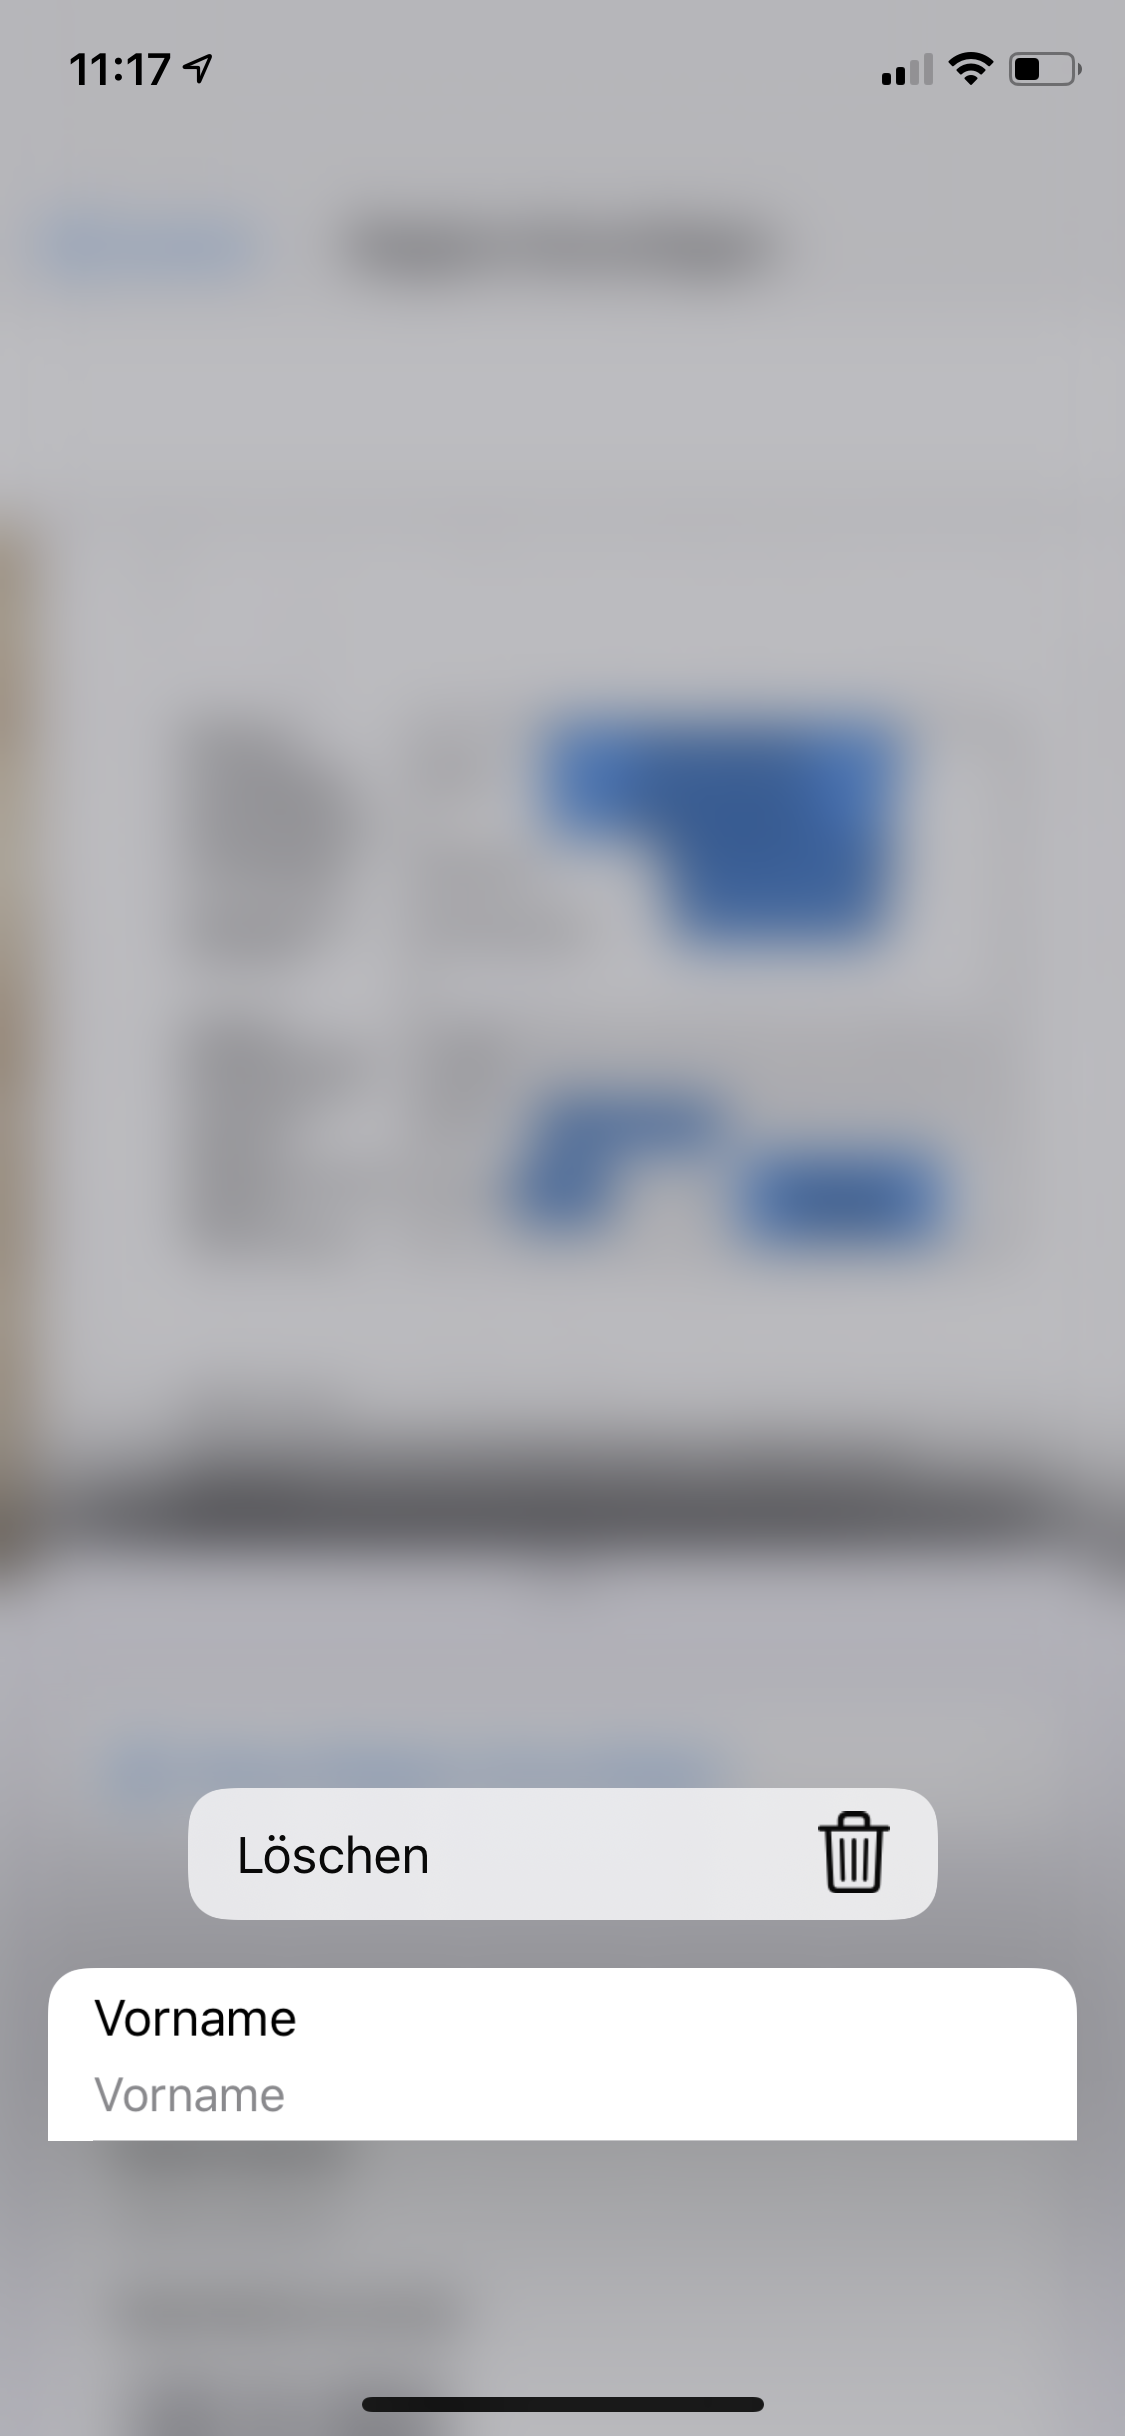
\includegraphics[width=0.96\textwidth]{img/V10}}
        			\caption{Löschen einer angelegten Region}
        			\label{fig:v10}
    			\end{subfigure}
    			\caption{Seiten-Vorschau-View}
				\label{fig:erstellung3}
			\end{figure}
			
			Im nächsten Schritt sind die Regionen auf den Dokumenten-Seiten zu markieren, deren Inhalt beim Einscannen digitalisiert werden soll. Zu erst wird die gewünschte Seite aus einer Übersicht (siehe \ref{fig:v4}) ausgewählt. Anschließend ist eine Vorschau der Seite mit alle eingetragenen Regionen zu sehen (siehe \ref{fig:v8} bzw. \ref{fig:v9}). Über einen Button können weitere Regionen hinzugefügt werden. Dazu legt man einen Namen (siehe \ref{fig:v5}) und einen Datentyp (siehe \ref{fig:v6}) fest. Die Datentypen sind für die Texterkennung und Erstellung der Tabelle für die Notenfreigabe wichtig. Dazu später noch mehr. Wenn die Eigenschaften der Region festgelegt sind, muss diese noch auf dem Bild markiert werden. Dazu zieht man mit einem Finger ein Rechteck in einer beliebigen Größe ein (siehe \ref{fig:v7}). Die markierte Region kann anschließend noch bewegt oder neu gemacht werden. Um kleinere Regionen präzise zu markieren kann mit einer Zwei-Finger-Geste auch an die Seite heran bzw. auch heraus gezoomt werden. Dieses Vorgehen muss dann für alle nötigen Regionen auf den jeweiligen Seiten wiederholt werden. 
			
			\begin{figure}[th]
    			\centering %%%%% LINKS!!!
				\begin{subfigure}[t]{0.3\textwidth}
       				\frame{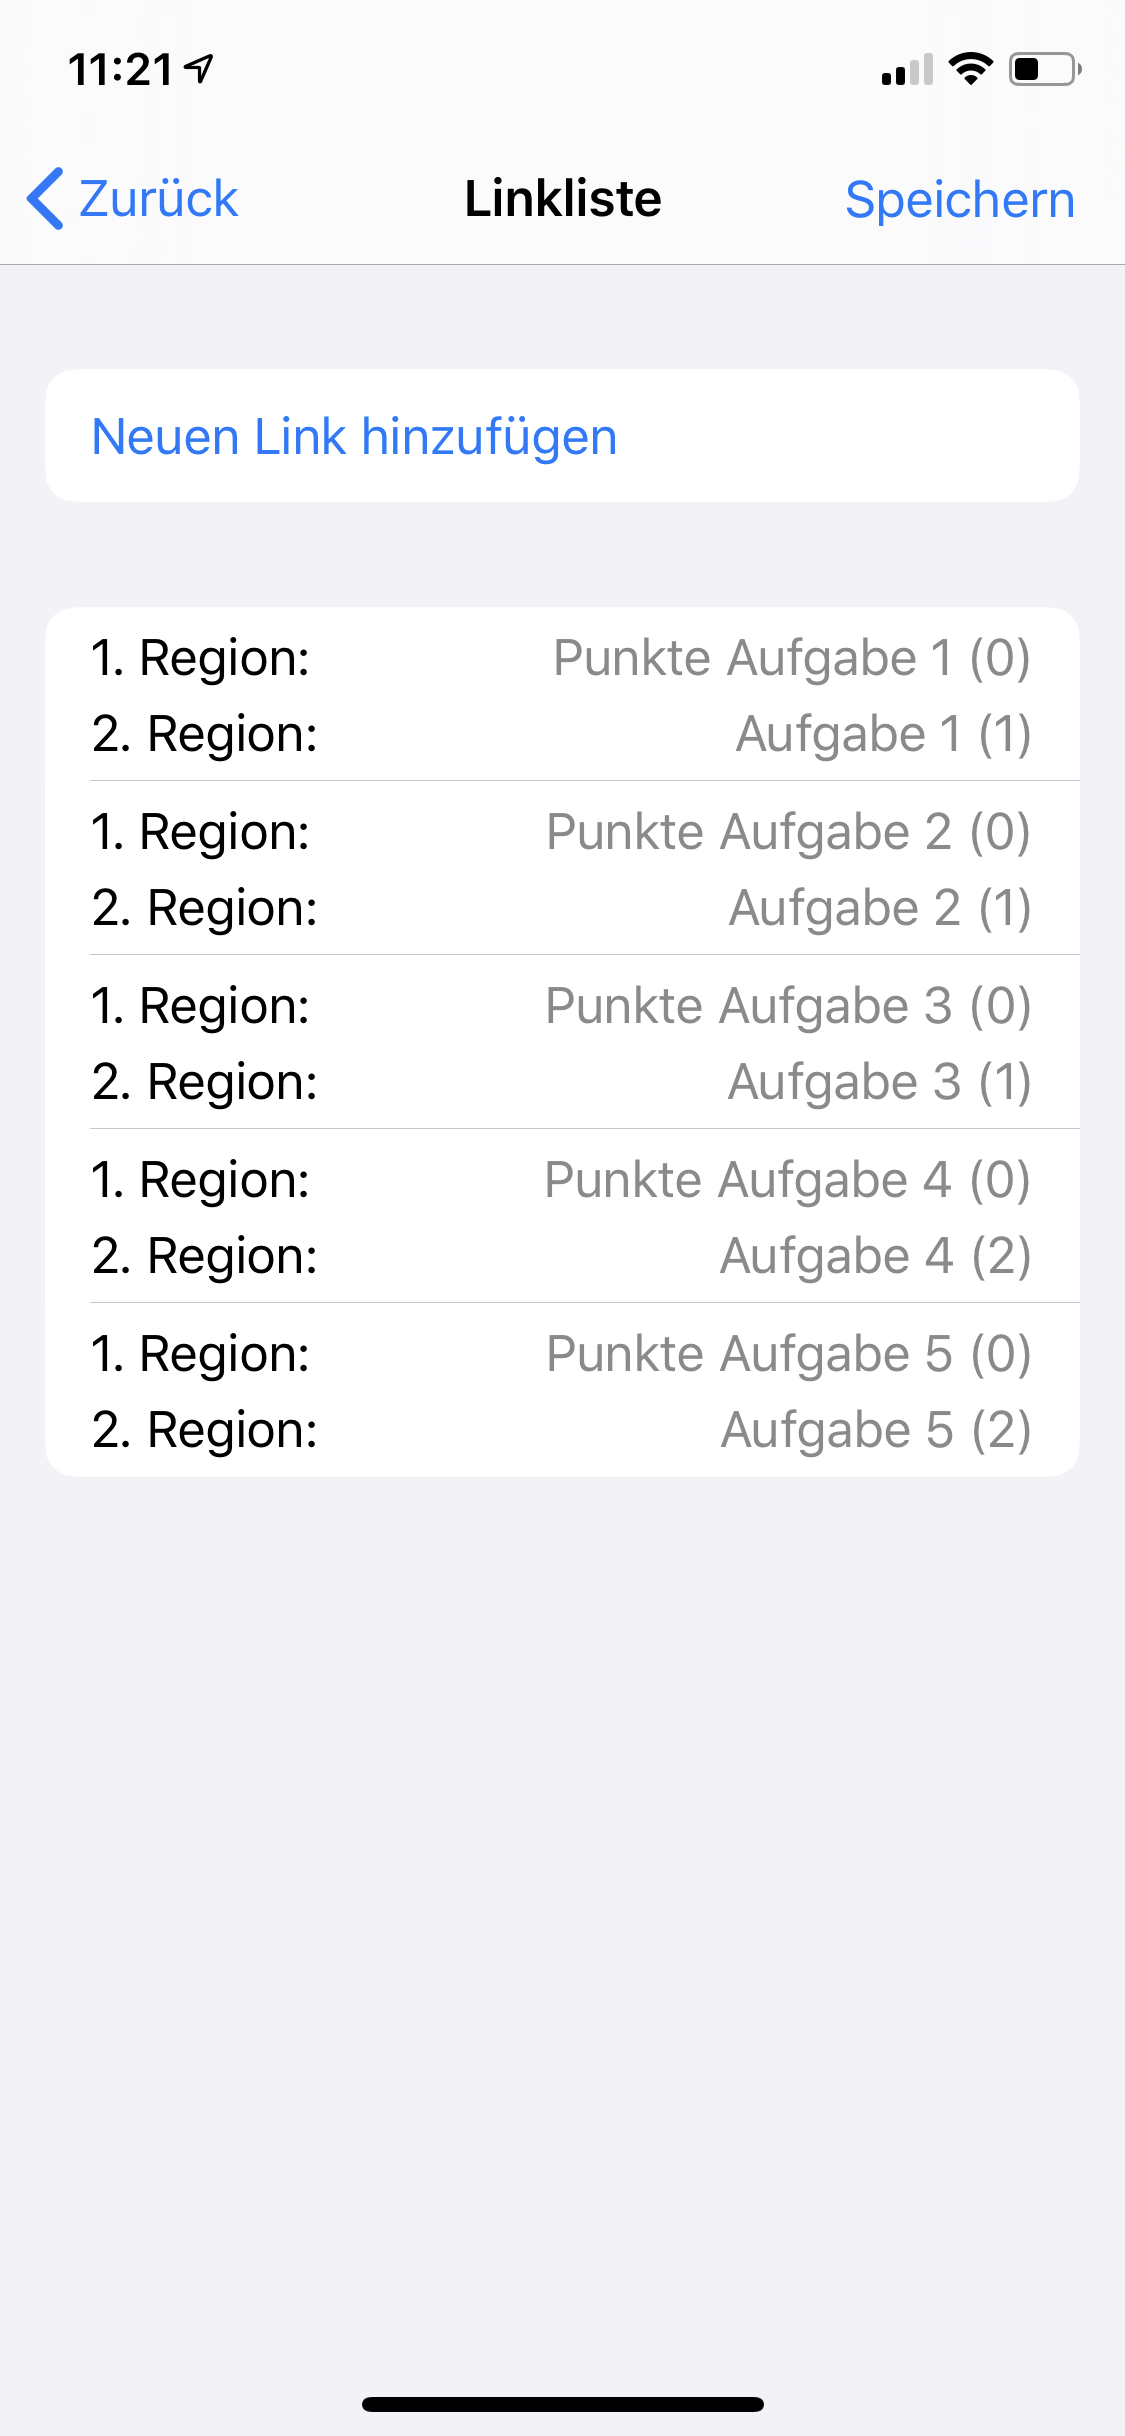
\includegraphics[width=0.96\textwidth]{img/L6}}
        			\caption{Linkliste mit angelegten Links}
        			\label{fig:l1}
    			\end{subfigure}
    			\begin{subfigure}[t]{0.3\textwidth}
       				\frame{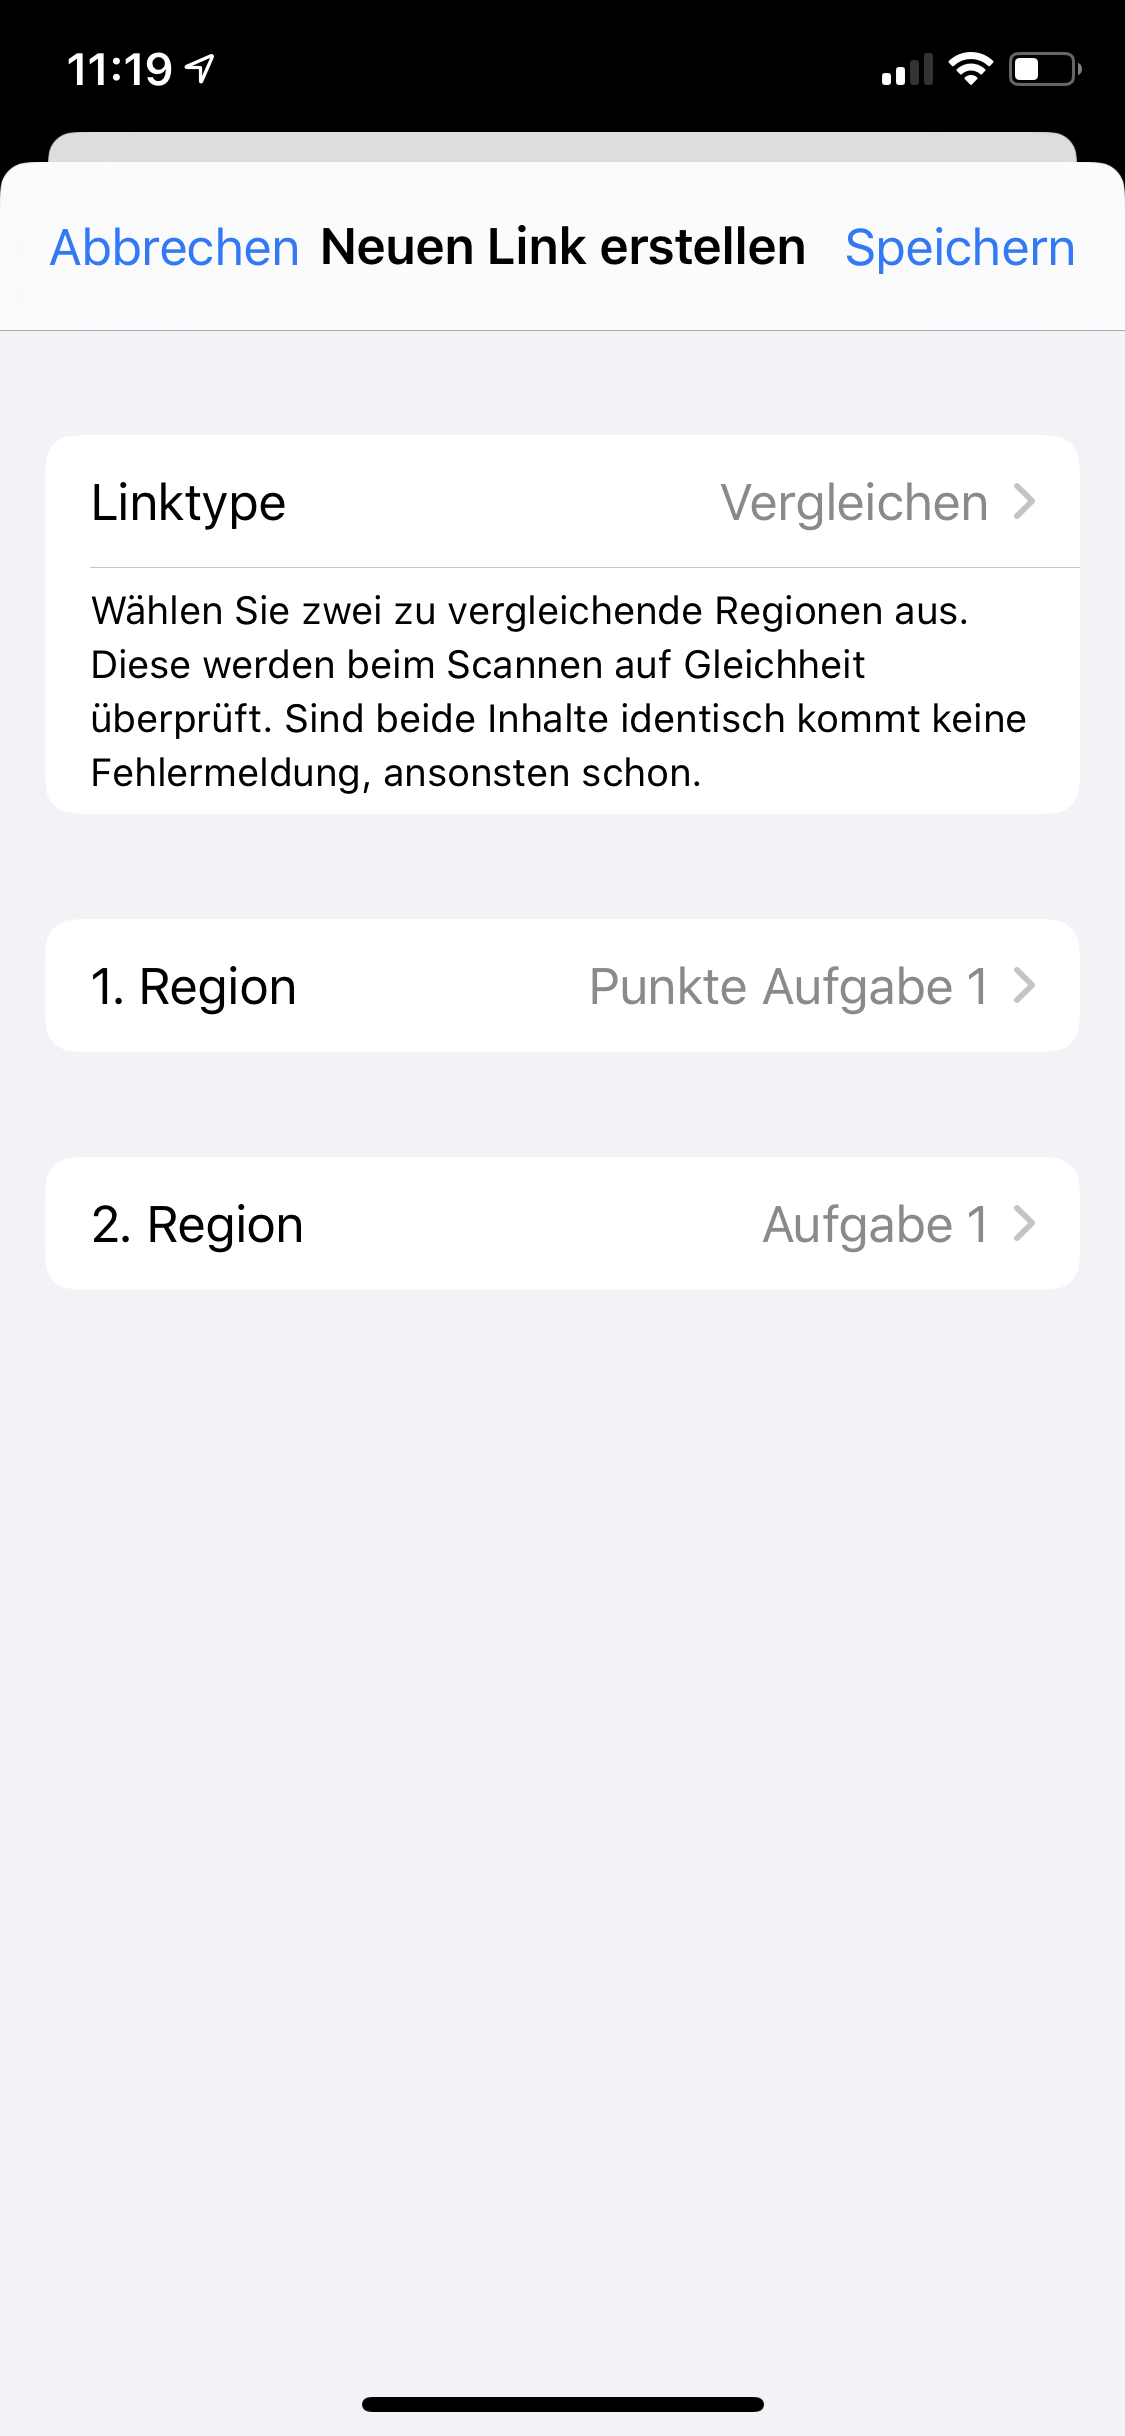
\includegraphics[width=0.96\textwidth]{img/L4}}
        			\caption{View zur Erstellung eines Vergleich-Links}
        			\label{fig:l2}
    			\end{subfigure}
    			\begin{subfigure}[t]{0.3\textwidth}
       				\frame{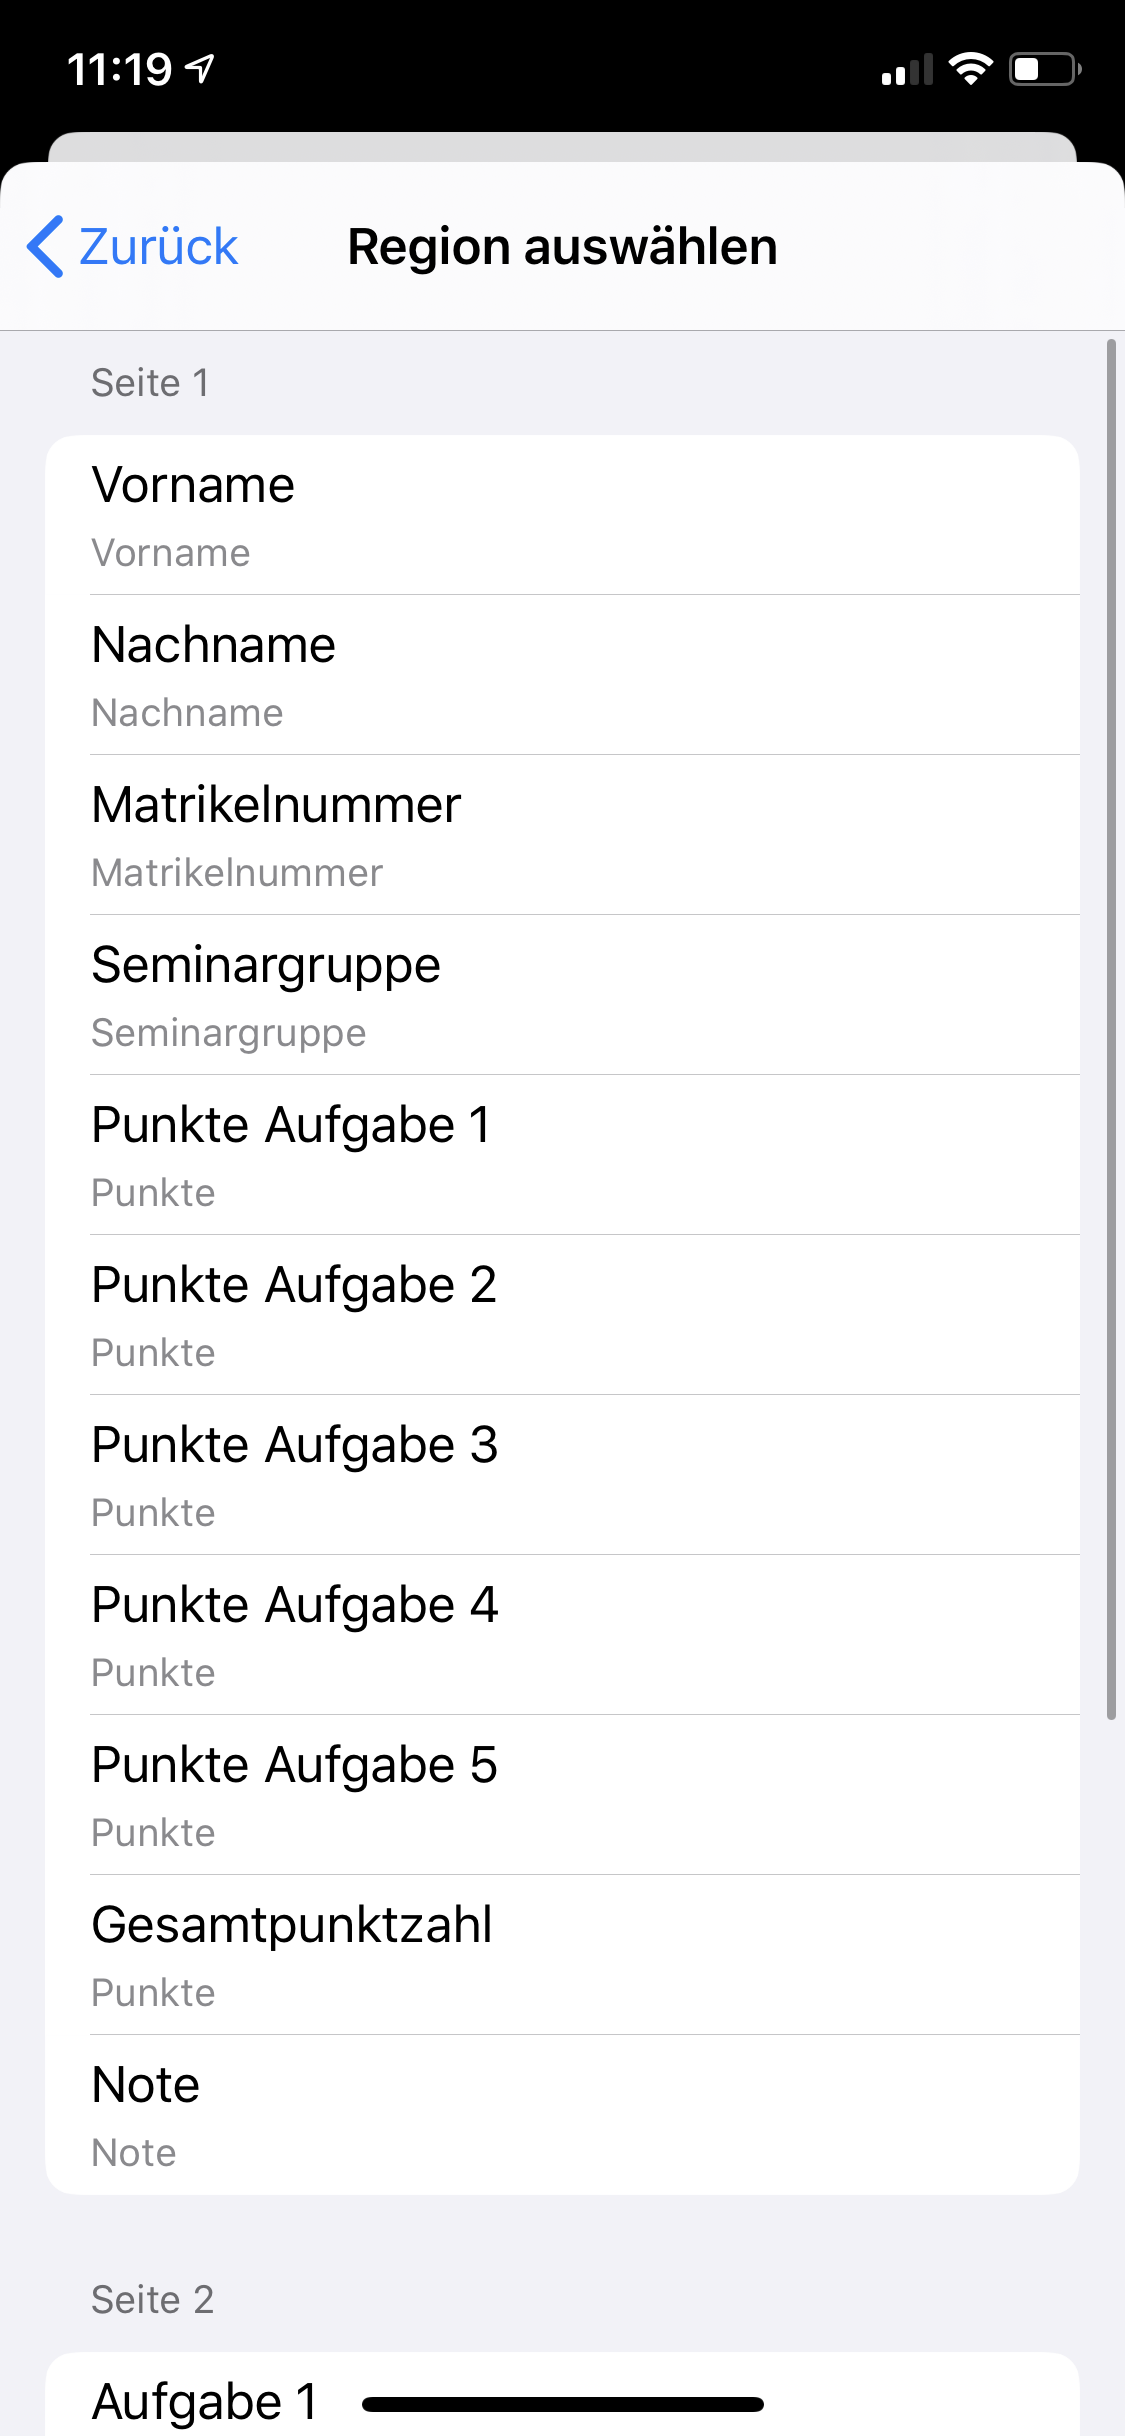
\includegraphics[width=0.96\textwidth]{img/L3}}
        			\caption{View zur Auswahl einer Region}
        			\label{fig:l3}
    			\end{subfigure}
    			\caption{Views zur Erstellung von Links}
				\label{fig:link1}
			\end{figure}

%%%%%%%%%%%%%%%%%%%%%%%%%%%%%%%%%%%%%%%%%%%% Bilder mit einbeziehen!		
			\subsubsection*{Links erstellen}
			Zum Schluss können noch die sogenannte Links erstellt werden. Diese Funktion ist allerdings noch nicht sehr weit fortgeschritten und beinhaltet aktuell nur den Link-Typ zum Vergleichen von Regionen, wie im \autoref{ch:konzept} beschrieben ist. Beim Erstellen eines Vergleich-Links wählt man zwei Regionen aus, deren Inhalt nach der Texterkennung auf Gleichheit überprüft wird. Genauer werden nur die IDs der Regionen in einem Link gespeichert. Diese werden dann, beim Einscannen benötigt, um den Inhalt der Regionen zu den IDs zu Analysieren. 
%%%%%%%%%%%%%%%%%%%%%%%%%%%%%%%%%%%%%%%%%%%% Bilder mit einbeziehen!
			\subsubsection*{Vorlage speichern}
			Wenn eine Vorlage gespeichert werden soll, passiert das in mehreren Schritten. Dazu wird die entsprechenden Server-Schnittstellen aufgerufen und auf die Server-Rückrufe gewartet. Für genauere Details zur API des Servers siehe im Praktikumsbericht von Tobias Kallauke.
			
			Im folgenden Abschnitt, ist beschrieben, in welcher Reihenfolge das Hochladen einer Vorlage zum Server geschieht. Dabei werden mögliche Fehler von Seiten des Server, der Internetverbindung und des Clients ignoriert. Jedoch ist im aktuellen Stand der App das Abfangen des Fehler schon integriert, die Fehlerbehandlung aber noch nicht.
			\begin{enumerate}
			%%%% LINKS!!!!
				\item Der Name und die Beschreibung der Vorlage sowie die Liste an Links wird gesendet. In der Antwort des Servers befindet sich  die Vorlagen-ID\nomenclature{ID}{Steht für einen einzigartigen Identifikator} , die in den nächsten Schritten benötigt wird. 
				\item Die Bilder der Seiten werden gesendet. Als Antwort zu jedem Bild wird der Pfad zurück geschickt, wo das Bild vom Server gespeichert wurde. Dieser Pfad wird im nächsten Schritt benötigt.
				\item Die Seiten mit einer Seiten-Nummer und dem Pfad zu dem Bild, wird mit der Vorlagen-ID gesendet. Als Antwort wird eine Seiten-ID zurückgegeben, die im nächsten Schritt verwendet wird.
				\item Die Regionen der Seiten werden gesendet. Eine Region hat X- und Y-Koordinaten. Diese repräsentieren den Abstand vom Bildursprung, der sich in jedem Bild oben links befindet. Außerdem besitzt eine Region noch eine Höhe und Breite sowie einen Namen und einen Datentyp (\ref{fig:v5} und \ref{fig:v7}). Die Koordinaten, sowie die Höhe und Breite sind alle in Pixel angegeben. Zusammen mit der Seiten-ID wird das Attribute an den Server gesendet.
			\end{enumerate}
			
		\subsection{Vorlage verwenden}
			Um eine Klausur zu digitalisieren, muss die vorher erstellte Scan-Vorlage ausgewählt werden (\ref{fig:liste1}). Danach bietet die Benutzeroberfläche über einen Button die Möglichkeit an, eine Klausur einzuscannen (\ref{fig:liste2}). Bevor die Bilder aufgenommen werden können, erscheint ein Dialogfenster (\ref{fig:ocr1}), in dem der Benutzer sich entscheiden muss, welche OCR-Engine benutzt werden soll. Aktuell gibt es zwei Möglichkeiten.
			\begin{itemize}
				\item Die OCR-Engine des Vision Framworks von Apple, welche direkt auf dem Gerät und ohne eine Internetverbindung die Texterkennung durchführt,  
				\item oder die OCR-Engine Tesseract, die über eine Schnittstelle des Servers aufzurufen ist.
			\end{itemize}
				
			\begin{figure}[th]
    			\centering
				\begin{subfigure}[t]{0.3\textwidth}
       				\frame{
\includegraphics[width=0.96\textwidth]{img/liste1}}
        			\caption{Übersicht aller Scan-Vorlagen}
        			\label{fig:liste1}
    			\end{subfigure}
    			\begin{subfigure}[t]{0.3\textwidth}
       				\frame{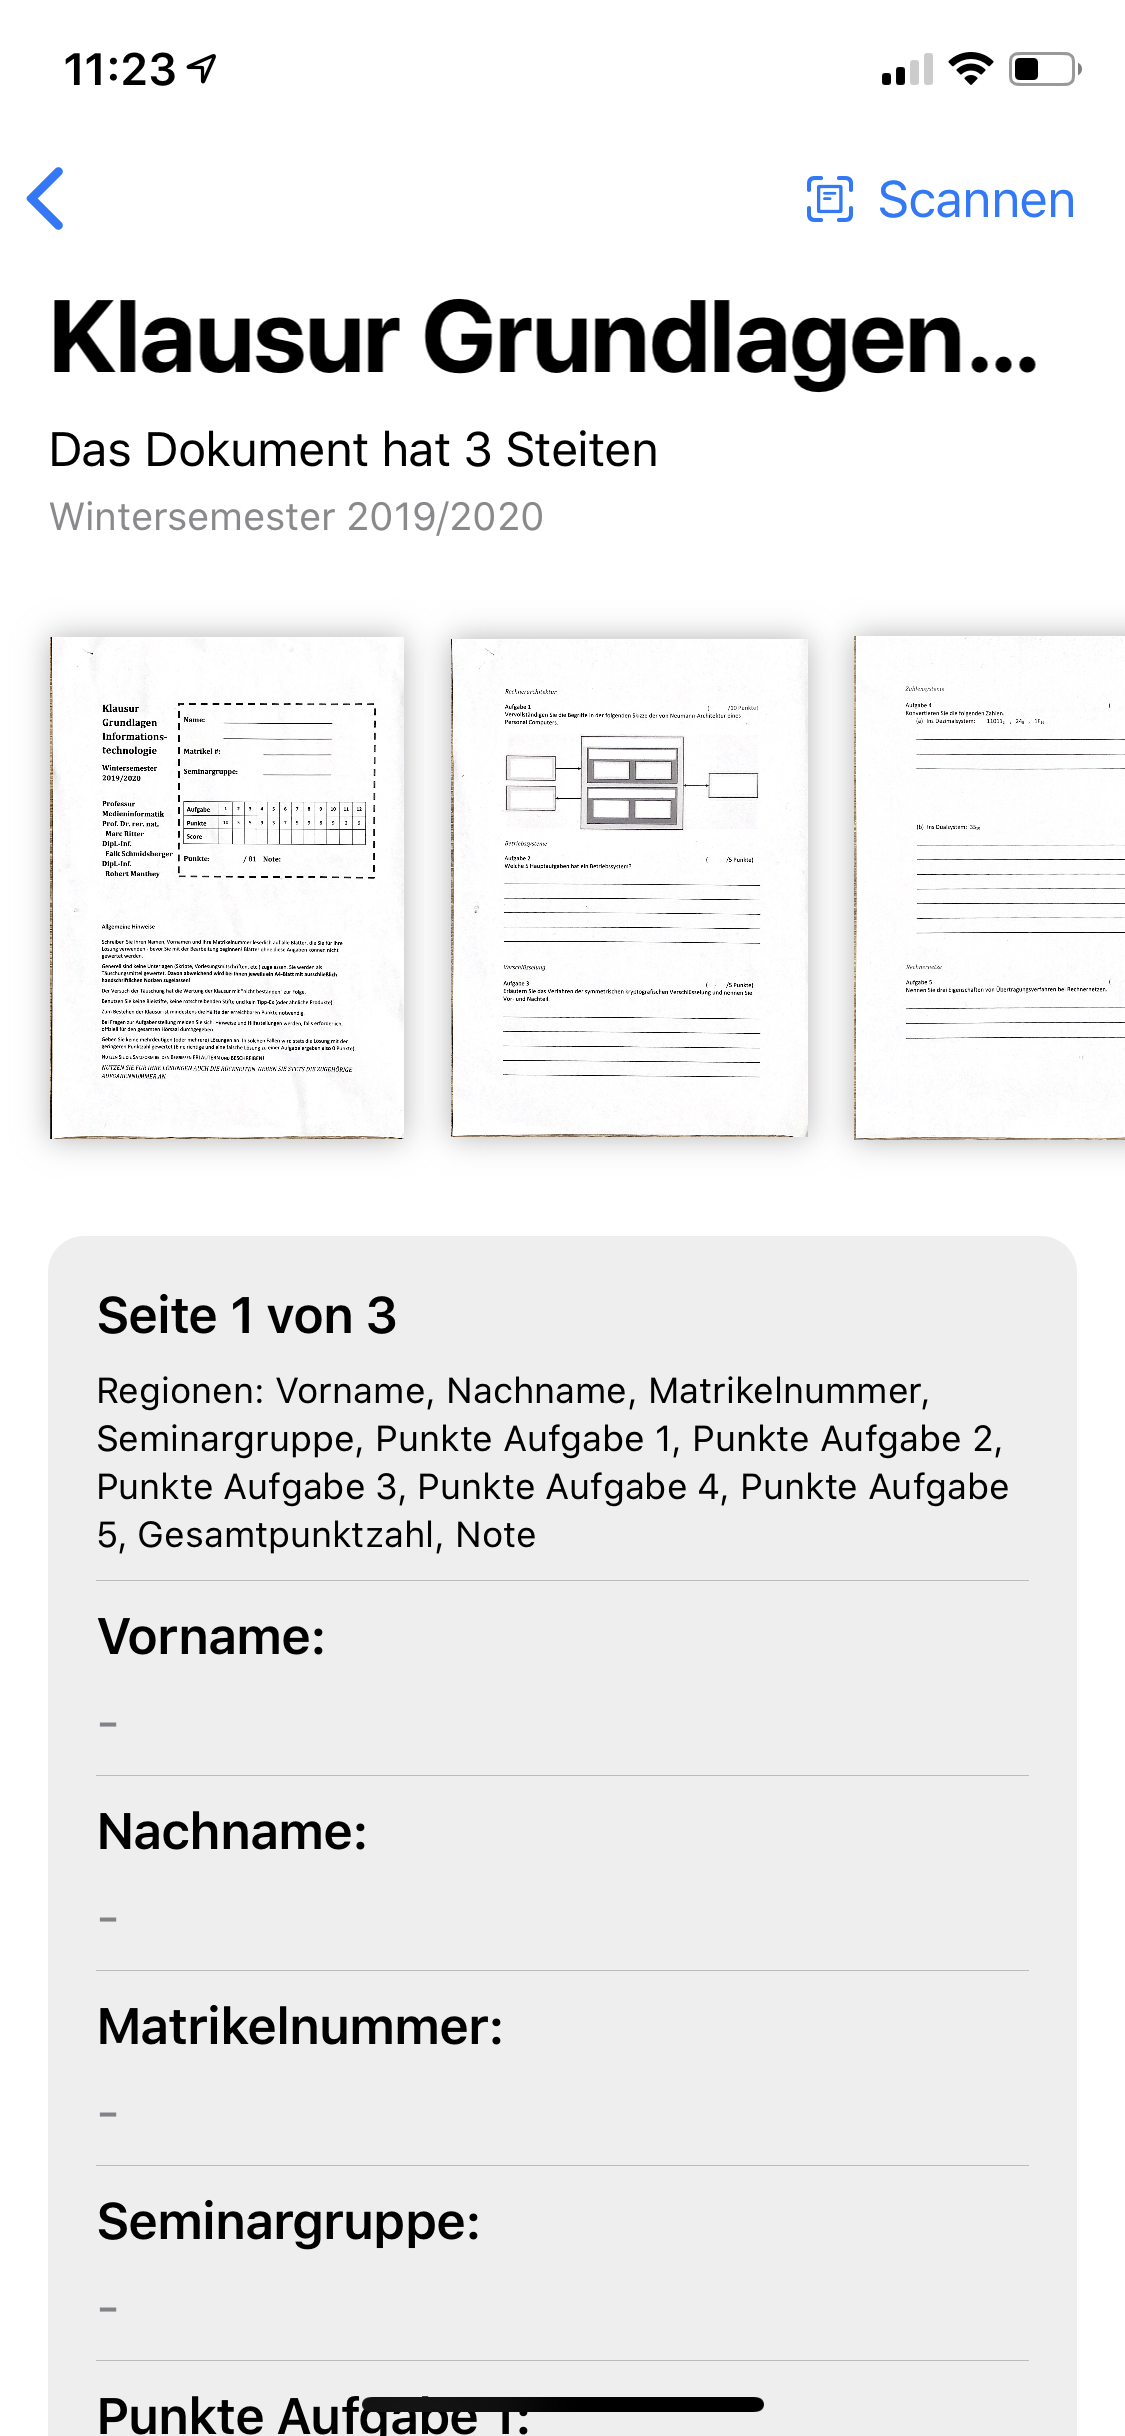
\includegraphics[width=0.96\textwidth]{img/liste2}}
        			\caption{Detailansicht einer Scan-Vorlage}
        			\label{fig:liste2}
    			\end{subfigure}
    			\begin{subfigure}[t]{0.3\textwidth}
       				\frame{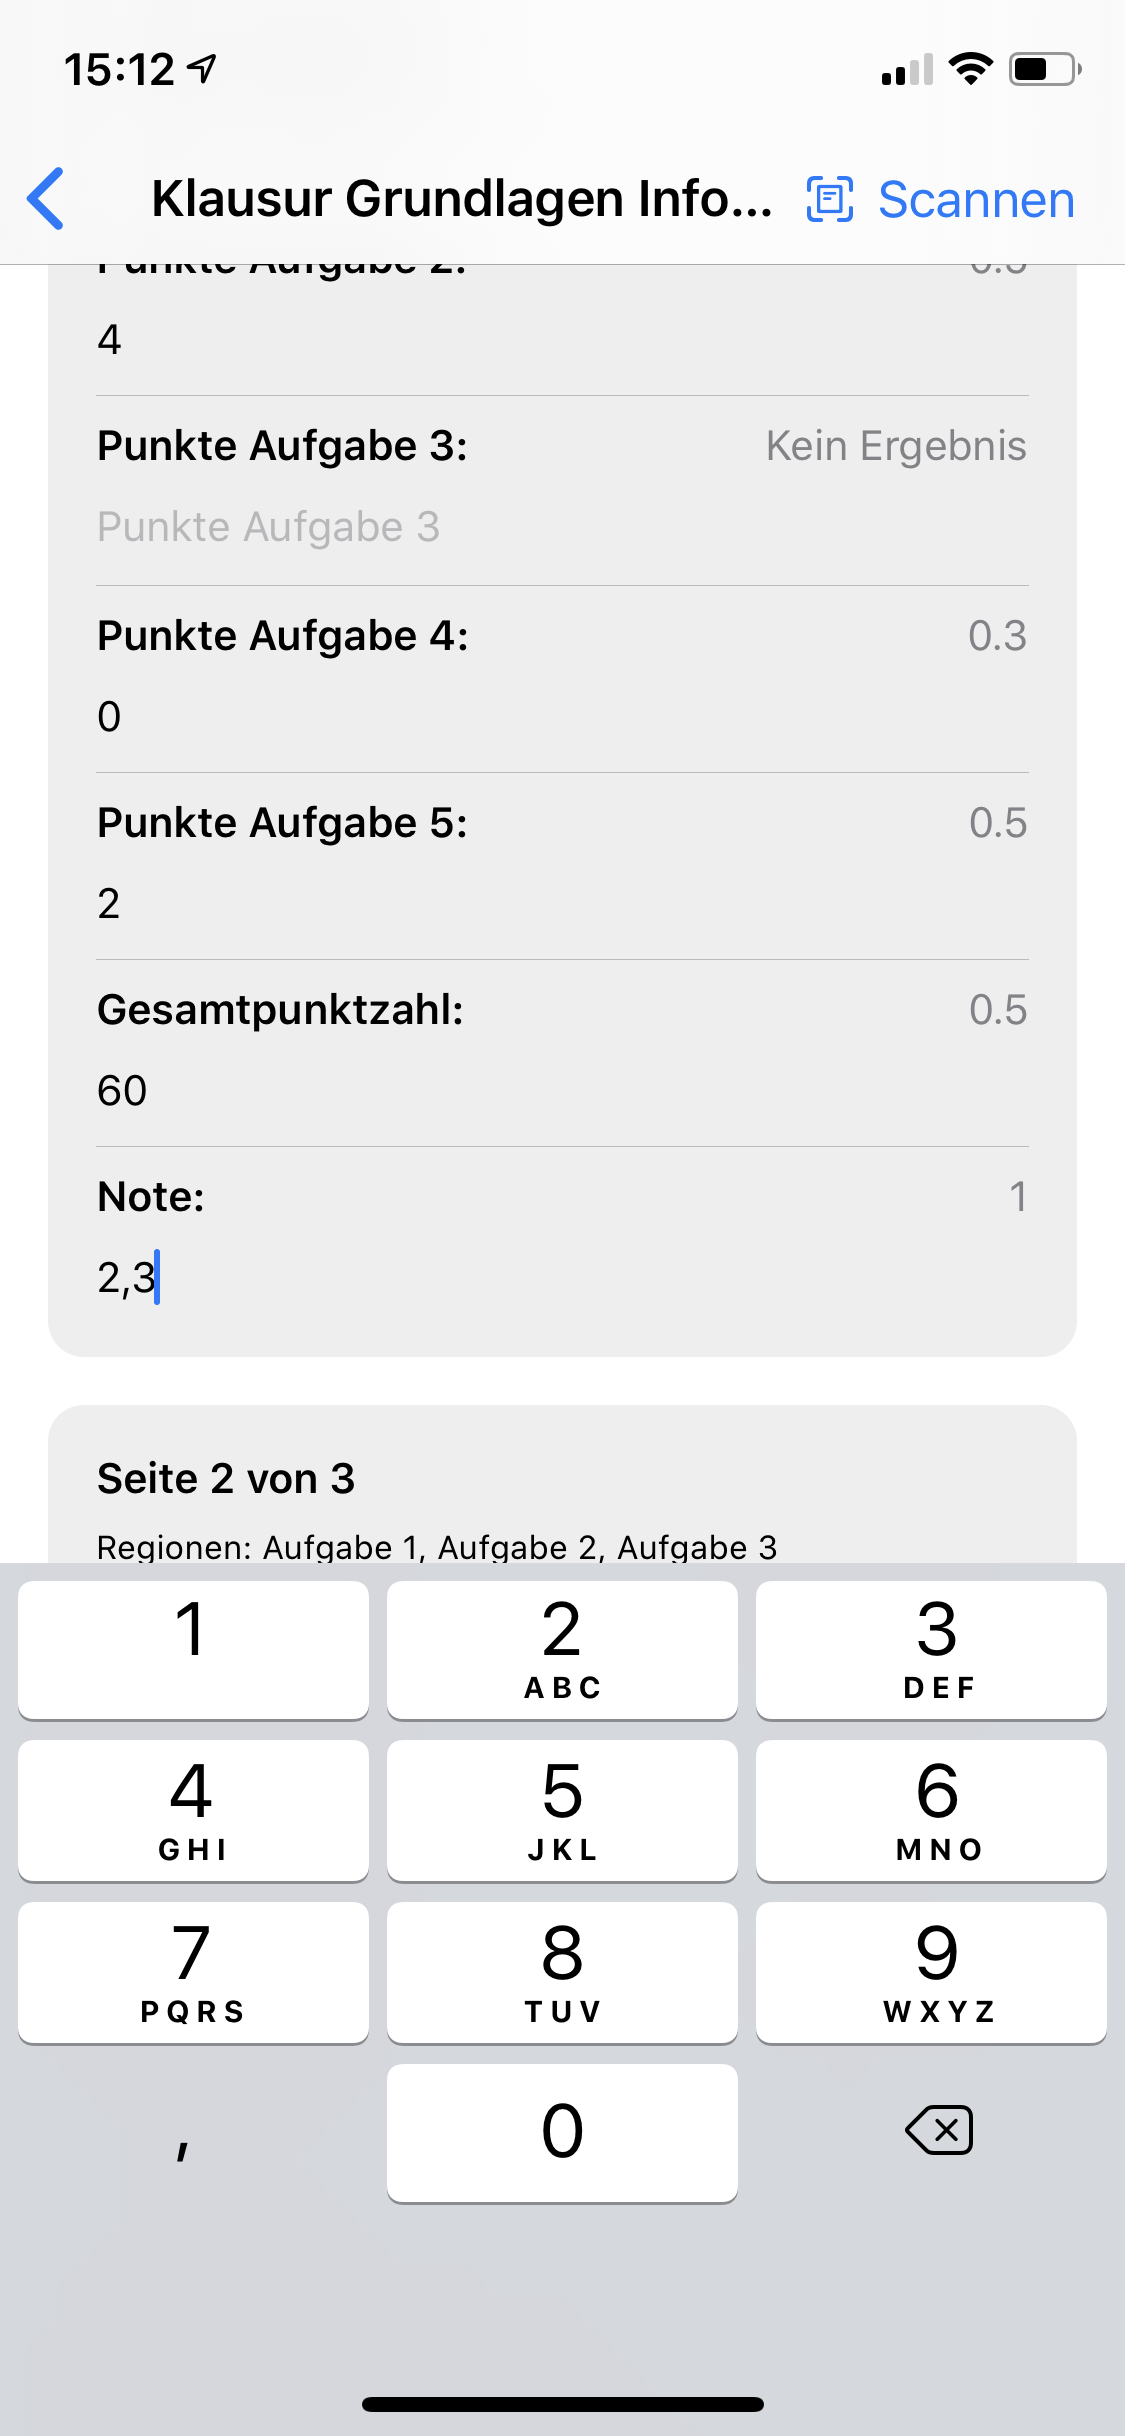
\includegraphics[width=0.96\textwidth]{img/ocr3}}
        			\caption{Liste der Links}
        			\label{fig:liste3}
    			\end{subfigure}
    			\caption{Listen- und Detail-Ansicht von Scan-Vorlagen}
				\label{fig:vorlagen}
			\end{figure}
			
			Nach der Auswahl öffnet sich die Kamera und die Bilder können aufgenommen werden. Wichtig dabei ist, dass die Seiten beim Fotografiert die selbe Reihenfolge, wie in der Scan-Vorlage haben. Auch muss die Anzahl der eingescannten Seiten mit denen in der Vorlage übereinstimmen. Bei der Implementierung der Scan-View wurde auf die Selbe zurückgegriffen, wie sie auch beim Vorlagen Erstellen zu finden ist (siehe \ref{fig:v3}). Grundsätzlich konnten viele Komponenten der gesamten Benutzeroberfläche dank SwiftUI immer wieder verwendet werden. Durch die Scan-View wird die Seiten aus dem Bild ausgeschnitten, geglättet und der Kontrast des Bildes wird ebenfalls leicht angepasst, damit Buchstaben leichter zu erkennen sind und Schatten bzw. Falten verschwinden.
			
			Nach dem Einscannen der Klausur-Seiten beginnt der Prozess der Texterkennung. Durch Aktivitätsanzeigen wird dem Benutzer mitgeteilt, dass die Anwendung gerade beschäftigt ist. Die Abläufe bei der online OCR-Engine sind jedoch leicht anders, als die, des Vision Frameworks.

			\begin{figure}[th]
    			\centering
				\begin{subfigure}[t]{0.3\textwidth}
       				\frame{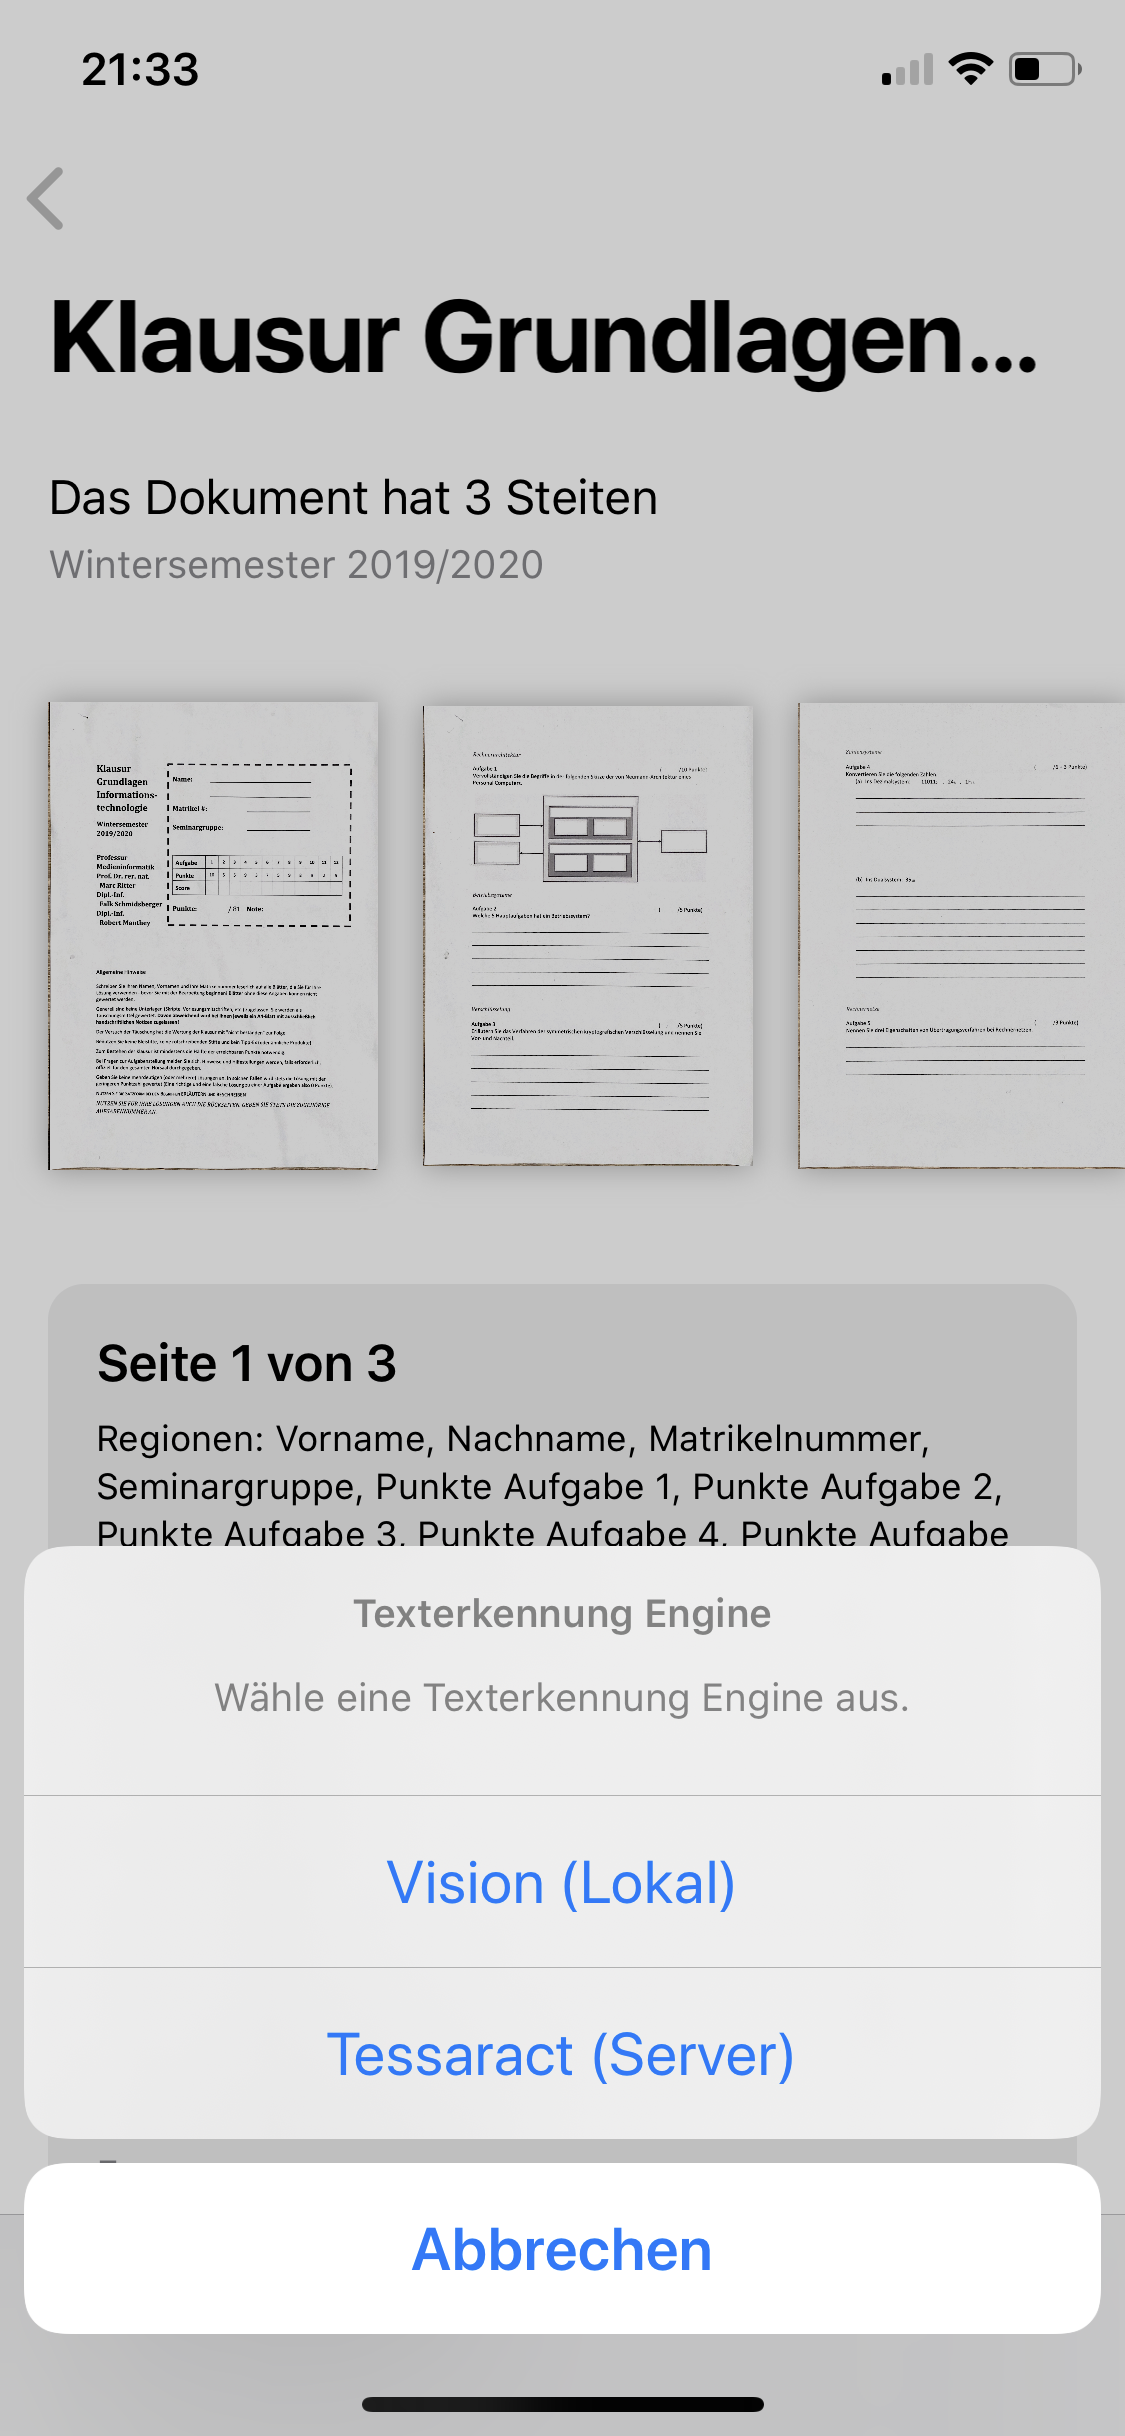
\includegraphics[width=0.96\textwidth]{img/ocr1}}
        			\caption{Dialogfenster zur Auswahl der OCR-Engine}
        			\label{fig:ocr1}
    			\end{subfigure}
    			\begin{subfigure}[t]{0.3\textwidth}
       				\frame{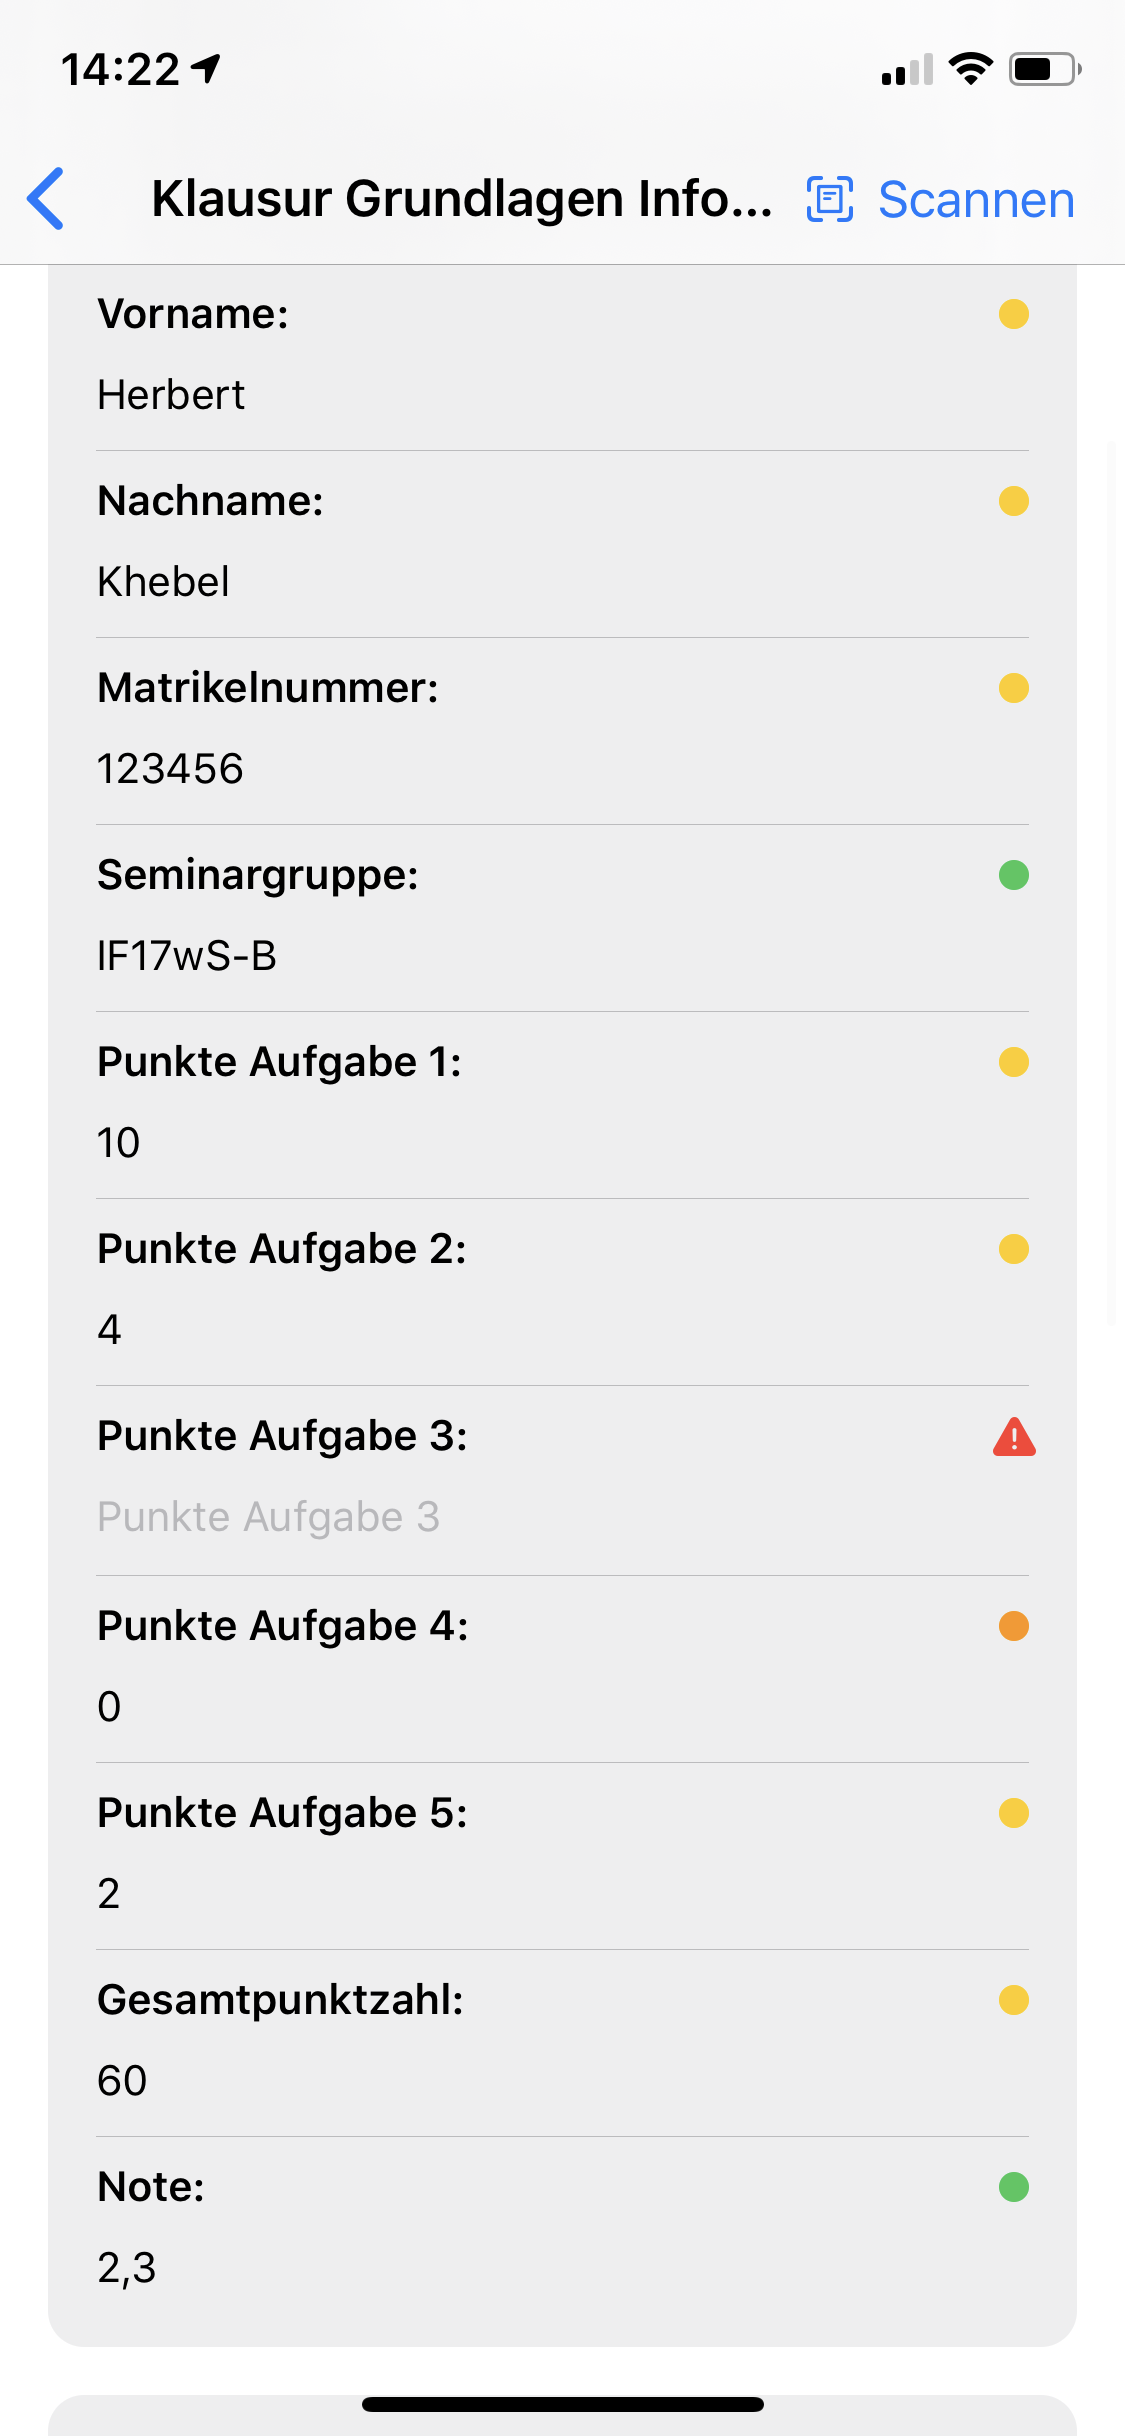
\includegraphics[width=0.96\textwidth]{img/ocr2}}
        			\caption{Übersicht nach der Texterkennung mit farblicher confidence}
        			\label{fig:ocr2}
    			\end{subfigure}
    			\begin{subfigure}[t]{0.3\textwidth}
       				\frame{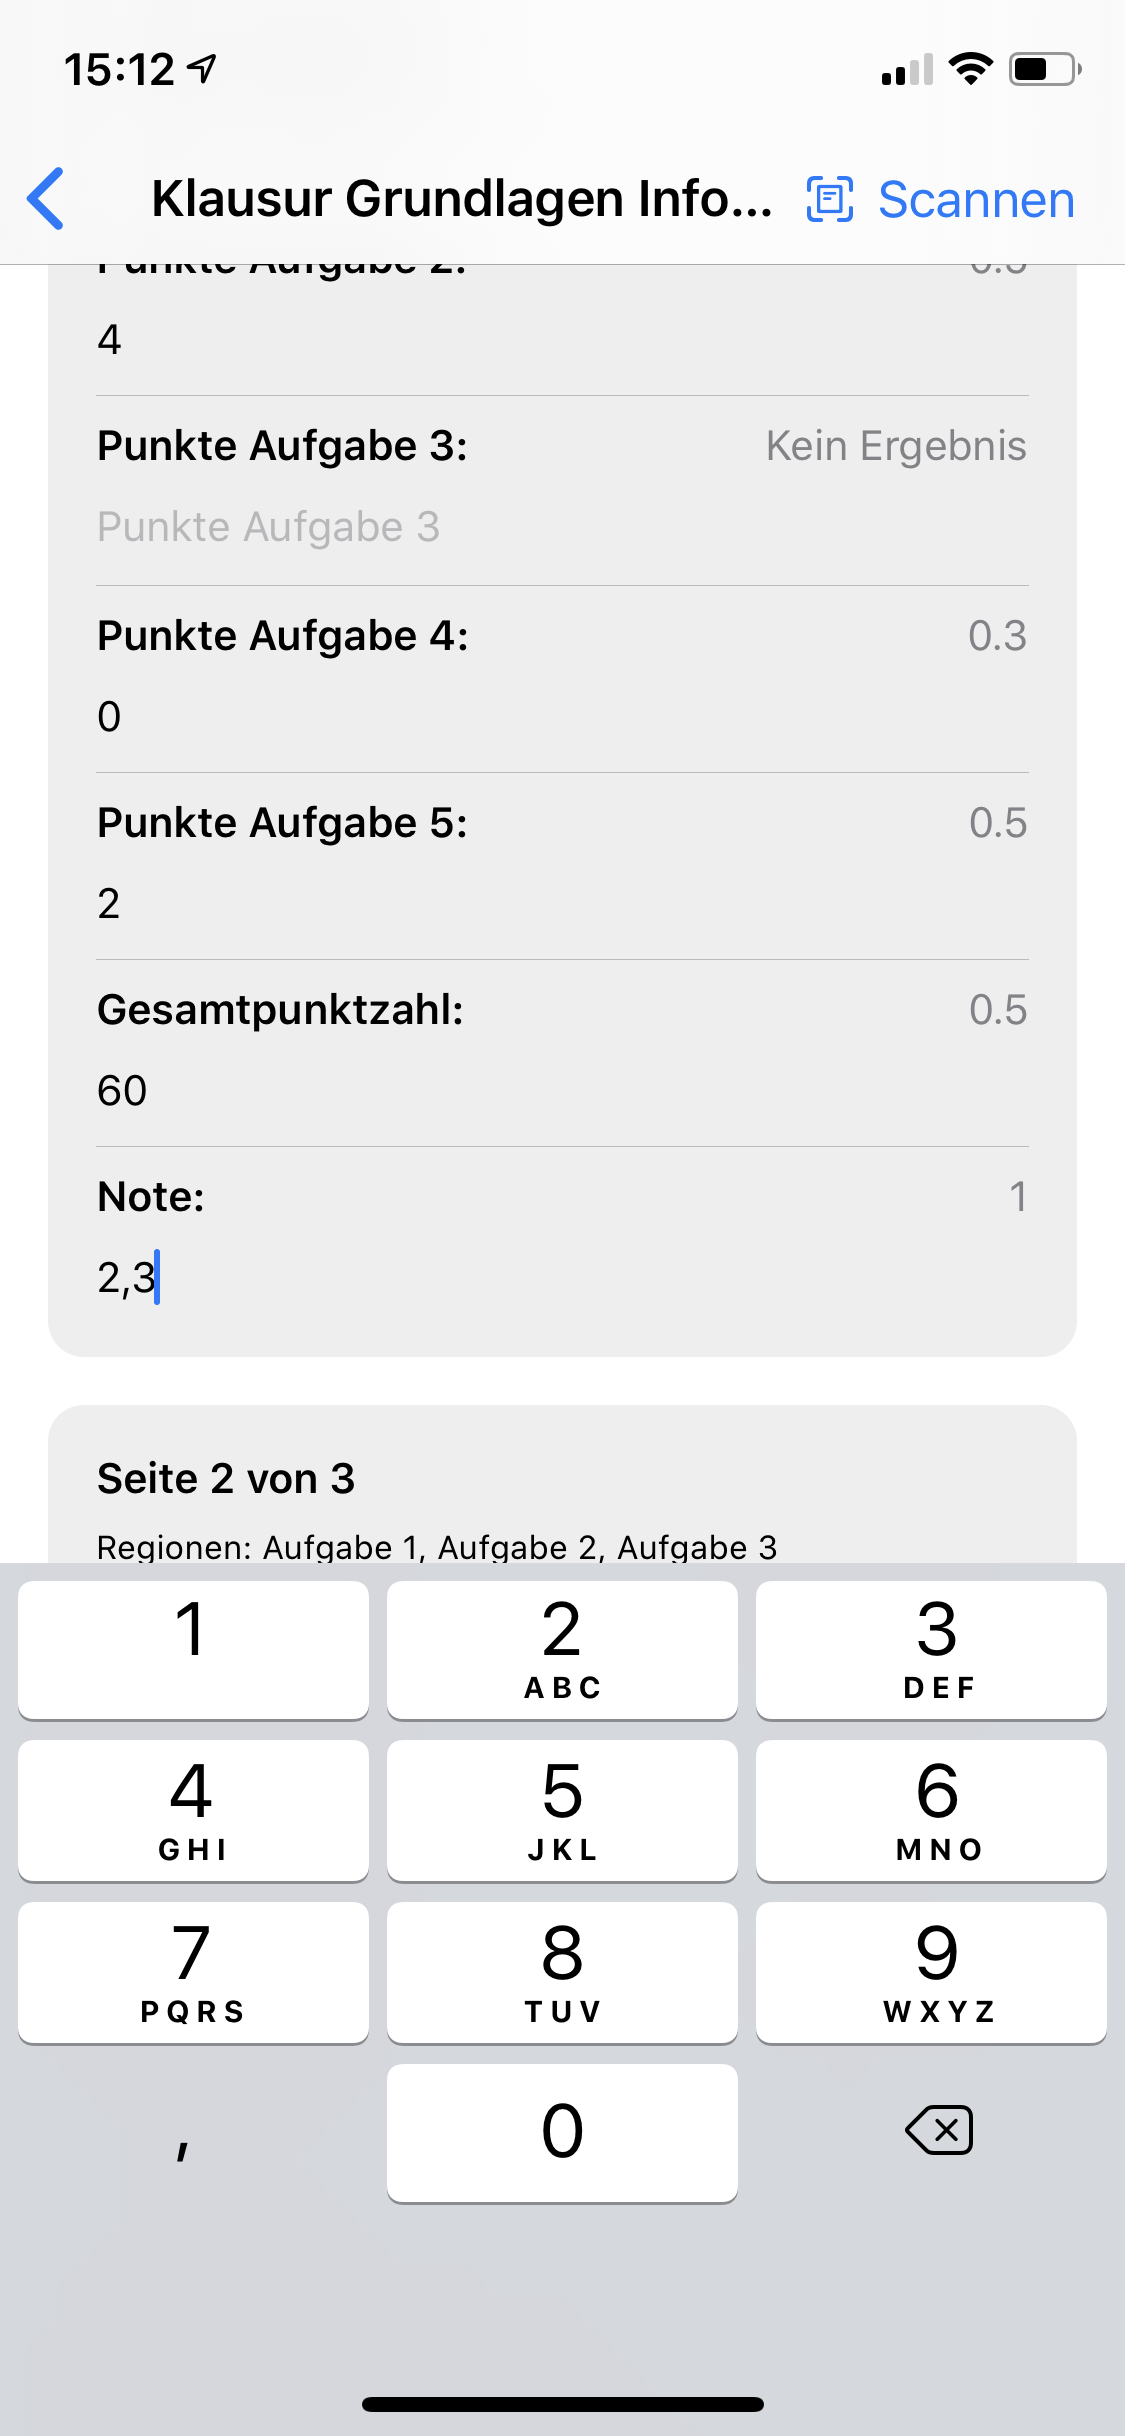
\includegraphics[width=0.96\textwidth]{img/ocr3}}
        			\caption{Änderung der Note mit spezieller Tastatur für Dezimalzahlen und confidence als Zahlenwert}
        			\label{fig:ocr3}
    			\end{subfigure}
    			\caption{Vorlagen-Ansicht vor und nach der Texterkennung}
				\label{fig:ocr}
			\end{figure}
			
			\subsubsection*{Ablauf mit Vision}
				Bei der Verwendung von Vision gibt es folgende grobe Schritte:
				\begin{enumerate}
					\item Die markierten Regionen in der Vorlage auf die neuen Bilder anwenden
					\item Mit den Regionen jedes Bilds Bildausschnitten erstellen
					\item Die Ausschnitte in die OCR-Engine geben
					\item Texterkennungs-Ergebnisse darstellen
				\end{enumerate}
			
				\paragraph*{Zu 1.: Die markierten Regionen in der Vorlage auf die neuen Bilder anwenden}
				Damit ist gemeint, dass nun das erste Bild des neuen Scans mit den Regionen der ersten Seite der Vorlage verarbeitet wird. Zur Erinnerung aus \ref{ch:konzept}: Das Ziel ist es, die markierten Regionen in der Vorlage auf die zu digitalisierende Seite anzuwenden und minimale Bildausschnitte zu erstellen, in denen der zu digitalisierende Text steht (siehe \autoref{fig:schema2}). Diese Ausschnitte werden dann von der Texterkennung verarbeitet. Diesen Vorgang wird für jede Seite wiederholt. Jedoch ergibt sich hierbei ein Problem.
				
				Wie man in den Abbildungen \ref{fig:seite1} und \ref{fig:seite2} sieht, haben beide, durch die App entstandenen Bilder, unterschiedliche Maße. Die \autoref{fig:seite1} ist größer und etwas breiter als die \autoref{fig:seite2}. Das liegt daran, dass sich der Winkel und der Abstand der Kamera zum Dokument bei den Aufnahme geändert hat, da das Gerät, während des Fotografierens in den Händen gehalten wurde. Das bedeutet also, wenn die Bilder in der Vorlage nicht genau so groß sind, wie die Bilder des neuen Scans, können im schlechtesten Fall wichtige Informationen durch die absoluten Positionen des Regionen abgeschnitten werden. Würde man immer den selben Abstand und Winkel garantieren, wie das beispielsweise in einem richtigen Kopiergerät oder Scanner der Fall ist, könnte man nun die Berechnung der absoluten Positionen in relative Positionen der Regionen weglassen. Zusätzlich sind die relative Höhe und Breite der Regionen ebenfalls zu berechnen. 

				\paragraph*{Zu 2.: Mit den Regionen jedes Bilds Bildausschnitten erstellen}
				Nachdem die neue Position und Maße aller Regionen einer Seite bestimmt sind, entstehen daraus Bildausschnitte für die Texterkennung. Zur Erinnerung, die Regionen dienen als eine Art Schablone, so dass alles, was sich außerhalb dieser befindet, nicht verwendet wird (siehe \autoref{fig:schablone1}). Auch trotz der Umrechnung in relative Positionen kann es bei falscher Erstellung der Vorlagen oder bei falschem Einscannen der Klausur passieren, dass trotzdem Teile der Regionen wegfallen. Für mehr Details über falsches Erstellen oder Einscannen siehe im \autoref{ssc:erkennen}.
				
				\paragraph*{Zu 3.: Die Ausschnitte in die OCR-Engine geben}
				Zu jedem Bildausschnitt wird eine sogenannte Texterkennungs-Anfrage konfiguriert. Auch hierfür wird immer noch die zugehörige Region des Ausschnitts benötigt. In der Konfiguration werden an Hand des Region-Datentyps (\ref{fig:v6}) unterschiedliche Einstellungen getroffen. Beispielsweise bekommt die Anfrage einer Region, vom Typ Note, eine Liste an möglichen Noten. Die Liste hat, wie schon im \autoref{ch:konzept} erwähnt, Vorrang vor dem Standard-Wörterbuch, in der Worterkennungsphase und sorgt für bessere Ergebnisse\footurl{Vision costumWords Dokumentation}{https://developer.apple.com/documentation/vision/vnrecognizetextrequest/3152640-customwords}. Auch könnte hier die Sprache des zu erkennenden Texts angegeben oder die  Texterkennungs-Stufe eingestellt werden. Diese bestimmt, welche Techniken bei der Texterkennung verwendet werden. Entweder man gibt der Geschwindigkeit Vorrang vor der Genauigkeit oder aber man setzt auf eine längere, rechenintensivere Erkennung. In der Anwendung ist die OCR-Genauigkeit entscheidend und auf die Einstellung der Sprache wurde verzichtet, da es sich in keinem Fall um normalen Text handelt, sondern um Eigennamen, Abkürzungen und Ziffern.
						
				Standardmäßig werden bei einer Texterkennungs-Anfrage zunächst alle Glyphen oder Zeichen im Eingabebild lokalisiert und dann jede Zeichenfolge analysiert\footurl{Quelle: VNRecognizeTextRequest Dokumentation}{https://developer.apple.com/documentation/vision/vnrecognizetextrequest}. Anschließend wird eine Korrektur an den erkannter Wörter auf der Grundlage eines Wörterbuchs und anderer Wahrscheinlichkeitsheuristiken für Zeichenpaare durchgeführt \cite{apple_text_2019}. Der genaue Ablauf der Texterkennung oder die verwendeten Algorithmen von Vision sind allerdings nicht bekannt. 
				
				Anschließend an die Texterkennung durch Vision erfolgt in einigen Fällen noch eine selbst entwickelte Korrektur, wie sie in \autoref{ch:konzept} \autoref{sc:erweiterungkonzept} beschreiben ist. Auch hier spielt der Regionen-Datentyp (\ref{fig:v6}) wieder eine Rolle. Beispielsweise wird der Text einer vermeidlichen Seminargruppe mit allen in der App hinterlegten Seminargruppen verglichen. Der Seminargruppen-Name mit der größten Übereinstimmung wird dann angezeigt. Die confidence wird ebenfalls angepasst. Zur Erinnerung, diese sagt aus, wie sicher sich die Texterkennung ist, dass das Ergebnis stimmt. Ähnliche Korrekturen gibt es für die Note und Punkte.
				
				Danach werden die erkennten Texte bzw. Worte und deren confidencen an den State-Container der App gesendet. Für die Ergebnisse der Texterkennung ist ein eigener State vorgesehen, in dem auch die Server-Ergebnisse von Tesseract gesichert werden. Somit ist das Anzeigen der Ergebnisse bei beiden OCR-Egines gleich.  
				
				\paragraph*{Zu 4.: Texterkennungs-Ergebnisse darstellen}
				Die Ergebnissen der Texterkennung und die jeweilige confidence werden auf der Benutzeroberfläche, nach Seiten sortiert, angezeigt (\ref{fig:ocr2}). Alle OCR-Ergebnisse können zudem noch angepasst werden. Abhängig vom Datentyp der Region passt sich die Tastatur beim Ändern der Texte an (\ref{fig:ocr3}). Beispielsweise sind die Tastaturen beim Anpassen von Noten und Punkte auf Zahlen und Dezimalpunkte spezialisiert. Zudem kann die confidence farblich (siehe \autoref{fig:ocr2}) aber auch als Zahlenwert (siehe \autoref{fig:ocr3}) angezeigt werden. Wurde kein Text erkannt, ist dementsprechend ein Warnsymbol an der Stelle der confidence zu sehen.    
 
			\subsubsection*{Ablauf mit Tesseract}
				Etwas anders ist der Ablauf, wenn die Texterkennung Tesseract auf dem Server verwendet wird:
				\begin{enumerate}
					\item Bilder an den Server senden
					\item Auftrag zur Texterkennung an den Server senden
					\item Serverseitige Texterkennung
					\item Texterkennungs-Ergebnisse darstellen
				\end{enumerate}
				
				\paragraph*{Zu 1.: Bilder an den Server senden}
				Nachdem das Dokument fotografiert wurden, werden die Aufnahmen an den Server gesendet. Dieser gibt, wie beim Speichern der Scan-Vorlage, die Pfade der Bilder als Antwort zurück. 
				
				\paragraph*{Zu 2.: Auftrag zur Texterkennung an den Server senden}
				Anschließend wird für jeden Pfad eine Auftrag zur Texterkennung an  die OCR-Schnittstelle des Servers gestellt. In der Anfrage wird der Pfad des Bildes und die passende Seiten-ID der ausgewählten Vorlage gesendet. Ab hier übernimmt der Server die Arbeit der Texterkennung.
				
				\paragraph*{Zu 3.: Serverseitige Texterkennung}
				Mithilfe der Seiten-ID, die in der Datenbank des Servers hinterlegt ist, werden dann die Regionen der Seite auf das Bild, welches sich an dem gesendet Pfad befindet, angewendet. Für mehr Details siehe im Praktikumsbericht von Tobias Kallauke. 
				
				\paragraph*{Zu 4.: Texterkennungs-Ergebnisse darstellen}
				Nach der Texterkennung sendet der Server die Ergebnisse der Seiten als Antwort zurück. Diese werden dann im selben State des State-Containers gesichert, wie es auch bei Vision der Fall ist. Die Ergebnisse bestehen aus der Region-ID, zur Zuordnung, dem erkannten Text, sowie der confidence des OCR, zu dem jeweiligem Wort. Auch ähnlich, wie es bei Vision der Fall ist. Die Darstellung der Ergebnisse und das Verhalten der Benutzeroberfläche ist ebenfalls identisch.      

%%%%%%%%%%%%%%%% - FAZIT - %%%%%%%%%%%%%%%

\chapter{Fazit}\label{ch:fazit}
	Dieses Kapitel reflektiert den aktuellen Stand der App und zieht einen Vergleich mit den Anforderungen aus \autoref{ch:anforderungen}.
	
	\section{Stand des Prototyps}
	
	Anforderungen: 
	
	- iOS die Klausuren digitalisiert 
	
	- tabellarisches Format
	
	- Texterkennung off und online
	
	- generischer Aufbau
	
	- Kontrollmechanismen /referenz zur implamentation, dort schon angesprochen
	
	- Anbindung an server -> nicht alles implentiert (ACHTUNG AUSBLICK)
	
	- Datenschutz und Datensicherheit-Richtlinien 

	Diese Kapitel reflektiert....
	
	Speichern der Ergebnisse nicht geschafft 
	
	Kontrolle der Ergebnisse vernachlässigt
	
	Fehlerbehandlung API
	
	\section{Hürden während der Entwicklung}
	
	- ein paar Worte, wie gut die Entwicklung lief (Simulator vs. echtes Gerät), wo sind die Grenzen des Simulators (Keine Kamera), wo waren Probleme mit dem echten Gerät...
	
	
	- jwt in KeyChain gesichert speichern 
	
	- GitHub actions
	
	- Debugging bei nicht statischen Daten schwer, Mock erstellen
	
	- Umfang von SwiftUI viele Umwege 


	\section{Probleme und Grenzen der App}\label{sc:grenzen}
		In diesem Abschnitt werden Probleme aufgeführt, die beim Verwenden der App beobachtet werden können. Auch wird hier über mögliche Lösungen zu einigen Problemen diskutiert.

		\subsection{Probleme beim Erkennen von Dokumenten}\label{ssc:erkennen}
			Bei der Erkennung von Dokumenten in einem Bild wird in der Bildverarbeitung auf Algorithmen der Segmentierung zurück gegriffen. Im Praktikumsbericht von Tobias Kallauke wird ein gängiger Ablauf zum Erkennen von Dokumenten dargestellt. Die genaueren Hintergrund und Schwächen der Algorithmen, welche die grundlegenden Probleme und Grenzen der App begründen, würden den Rahmen des Praktikumsberichts sprengen, weshalb darauf nicht weiter eingegangen wird. Allerdings muss klar sein, dass für die Erkennung des Dokuments es wichtig ist, dass die Ecken sowie die Seiten sich gut vom Hintergrund abheben.
		
			Das bedeutet im Umkehrschluss, dass wenn die Seiten und Ecken sich nicht gut abheben, kann das Dokument nicht oder nur schlecht erkannt werden. Allerdings gibt es für diese Probleme zwei effiziente Lösungen. 
			\begin{itemize}
				\item Die erste Lösung besteht darin, einen Blitz zu verwenden. Meistens schaltet sich bei zu wenig Licht die zusätzliche Belichtung automatisch ein. Grundsätzlich empfiehlt es sich aber, immer eine Blitz zu verwenden, da dadurch das Dokument gleichmäßig belichtet wird. Außerdem werden Schatten vom Benutzer oder durch kleinere Falten beseitigt, welche durch eine Deckenbeleuchtung entstehen könnten. Bei einer zu starken Grundbelichtung verschlechtert ein Blitz jedoch nur das Ergebnis, da dadurch Text und Kanten unkenntlich gemacht werden könnten. Nach eigener Erfahrung ist es am geeignetsten, bei Tageslicht und mit Blitz die Dokumente aufzunehmen. 
				\item Auch wenn bei guter Belichtung, die Wahrscheinlichkeit für falsche Kantenerkennung reduziert worden ist, kommt es bei schnellen Bewegungen der Kamera oder zu spitzem Winkel zum Dokument sowie ungeeignetem Hintergrund trotzdem dazu, dass ein falscher Bildausschnitt als Dokument gewählt wird. Deshalb ist es möglich das Bild noch einmal aufzunehmen, oder aber das Dokument im Bild selbst zu markieren. Dafür stellt VisionKit eine besondere View zur Verfügung, die es einem ermöglicht, die Ecken des Dokuments per Hand auszuwählen. Das hilft auch gegen die Problematik, wenn die Ecken des Papiers umgekickt oder abgerissen sind, da man selbst die Position der Ecke approximiert angeben kann. 
			\end{itemize}
		
		\subsection{Probleme der Klausur-Vorlage beim Scannen}\label{ssc:problemevorlage}
			Dieser Abschnitt bezieht sich ausschließlich auf entstandene Probleme mit der Klausur, welche in \autoref{fig:klausur} zu sehen ist. Diese stand während des Praktikums als Beispiel-Klausur zur Verfügung und ist stellvertretend für alle Klausuren-Vorlagen der Fakultät CB. Im \autoref{sc:vorlage}, werden mögliche Änderungen und Lösungen zu den hier aufgeführten Problemen diskutiert.
		
			Wie in der \autoref{fig:seite1} zu sehen ist, besitzt die Klausur ein Deckblatt mit Feldern, die der Student auszufüllen hat. Darunter Name, Artikelnummer und Seminargruppe. Diese Informationen sind essentiell bei der Digitalisierung und doch wird nicht klar zwischen einem Feld für den Vornamen und einem Feld für den Nachnamen differenziert. In den Abbildungen \ref{fig:erstellung2} und \ref{fig:erstellung3} wird diese Problematik nochmal dargestellt. Bei den Datentypen der Regionen (\ref{fig:v6}) wird zwischen Vornamen und Nachnamen unterschieden, auf der Klausur (\ref{fig:v7}) jedoch nicht. In der abgebildeten Vorlage (\ref{fig:v9}) wurde der Vorname auf den ersten und der Nachname auf dem zweiten Strich des Feldes Namen gesetzt. Auch verleitet ein einzelner Strich dazu, über die Länge hinaus zu schreiben. Wenn die Regionen der Scan-Vorlage dann zu klein gewählt ist, können Informationen fehlen. Bei dem Feld für die Note wird dies noch extremer. Da nicht mal ein Markierung für die Note vorhanden ist, müsste man einen sehr viel größeren Bereich markieren (\ref{fig:v9}). Allerdings wird hinter der Note auch die Unterschrift des Prüfers gesetzt, welche bei der Digitalisierung nicht mit auftauchen sollte. Im Gegensatz dazu sind die Felder in der Tabelle für die Punkte zu jeder Aufgabe zu klein. Die geringe Größe verleitet dazu, dass Feld komplett aus zu nutzen und die Ziffer möglichst groß rein zu schreiben. Dazu kommt dass solch kleinen Regionen kaum Spielraum für Toleranz lassen und somit entstehen hier immer wieder Fehler. Entweder die Ziffer ist abgeschnitten, wenn man die Region zu klein wählt oder aber die Ränder des Feldes werden als eine Eins oder als der Buchstabe l erkannt, wenn man die Region zu groß wählt.

		\subsection{Weitere Probleme der App}
			Obwohl SwiftUI die Entwicklung der App erst möglich gemacht hat, bringt das Framework von Juni 2019 einige Schwierigkeiten mit sich. Seit der Veröffentlichung gibt es nur eine sehr kleine Dokumentation und der Schnitstellen-Umfang, kann auch noch lange nicht mit dem des Frameworks von UIKit mithalten, welches seit Jahren in der iOS-Entwicklung als Standard benutzt wird. Grund für den geringen Umfang und schlechter Dokumentation ist vermutlich, die ständige Weiterentwicklung Seitens Apple. Das führt jedoch zu einigen provisorischen Lösungen und macht das Auffinden von Fehlern besonders schwierig. Deshalb kann es bei der Benutzung der App zu unerwarteten Abstürzen oder Aufhängern kommen. Des Weiteren sind die verwendeten Texterkennung-Engines nur für gedruckte Schrift ausgelegt. Handschriftliche Zeichen werden nur dann gut erkannt, wenn sie in Druckschrift geschrieben sind. Bei Ziffern ist es besonders auffällig, da z. B. eine gedruckte 4 oder 7 ganz andere Charakteristiken haben, als wenn sie geschrieben wurde.
	
	%%%%%%%%%%%%%%%% - TEMPLATES - %%%%%%%%%%%%%%%

	\section{Verbesserung der Klausuren-Vorlage}\label{sc:vorlage}
		% War in der Problemstellung drin... konnte nicht begonnen werden -> Ausblick BA
	
		Dieser Abschnitt beschäftigt sich mit Verbesserungen und Änderungen an Hand der Klausur in \autoref{fig:klausur}. Sie steht jedoch stellvertretend für die Klausuren-Vorlage der Fakultät CB. Alle folgenden Vorschläge haben den Hintergrund die App bei der Digitalisierung zu unterstützen und basieren auf der gesammelten Erfahrung mit der Anwendung, während der Entwicklung sowie den angegeben Problemen aus \autoref{sc:grenzen}.
	
		Der erste Vorschlag bezieht sich auf die Problematik, dass die Ecken und Kanten bei der Erkennung des Dokuments entscheidend sind. Sie sind die wichtigsten Referenz-Punkte bei der Objekt-Erkennung, können aber unter bestimmten Bedienungen, wie im \autoref{ssc:erkennen} erklärt, nicht immer erkannt werden. Aus diesem Grund empfiehlt es sich eigene Referenzpunkt auf dem Dokument anzubringen. Beispielsweise durch einen Rahmen, wie es schon auf der Klausur (\ref{fig:seite1}) gemacht wurde, oder durch QR-Code ähnliche Muster. Der Vorteil bei eigenen Referenzpunkt ist, dass sie so gestaltet werden können, dass sie sich immer vom Blatt abheben. So mit ist die Dokumenten-Erkennung nur noch vom Licht abhängig. Ein weiterer Vorteil ist, dass dadurch die Kamera noch näher an den Text heran kann und die Auflösung noch besser wird. Der größte Nachteil daran ist allerdings, dass die Erkennung nicht mehr allein von Frameworks übernommen werden kann. Es müsste ein neuronales Netz trainiert werden, welche diese Referenzpunkte in Bildern erkennt. 
	
		Der zweite Vorschlag bezieht sich auf den \autoref{ssc:problemevorlage}. Einige dort angesprochenen Probleme bezogen sich auf die Ungewissheit, wie groß eine Region abzustecken ist. Die einfachste Lösung ist es, einen genauen Rahmen für alle Felder fest zu legen. Auch müssen alle Felder ausreichend beschriftet sein, so dass jedem klar ist, wo was hineinzutragen ist. Und um das Problem zu vermeiden, dass der Rahmen als ein Buchstabe oder eine Zahl erkannt wird, kann dieser nur schwach eingezogen werden. Mithilfe von Bildverarbeitung-Algorithmen könnten diese feinen Linien dann auch ohne Verlust der wichtigen Daten heraus gerechnet werden. 


%%%%%%%%%%%%%%%% - AUSBLICK - %%%%%%%%%%%%%%%
		
% Jedoch sollten auch einige angesprochenen Probleme aus Kapitel \ref{ch:grenzen} behoben werden, wenn die App in Zukunft tatsächlich von Hochschulmitarbeitern benutzt werden soll.
\chapter{Ausblick}
	Der aktuelle Stand der App bietet eine gute Grundlage für mögliche Weiterentwicklungen. Jedoch fehlen einige wichtige Elemente zur Inbetriebnahme des Software-Systems, wie schon im \autoref{ch:fazit} verdeutlicht. In den folgenden Abschnitten wird von dem Zustand der Software abgesehen und einige Ideen erläutert, wie die App und das gesamte Software-System weiter entwickelt und verbessert werden kann.

	\paragraph*{Verbesserung der Benutzerfreundlichkeit und des Workflows} Gerade weil die App noch ein Prototyp ist, sollten bei einer Weiterentwicklung zu allererst Dinge implementiert werden, die die Benutzung verbessern. Beispielsweise werden Login-Daten und schon gedownloadete Vorlagen nicht gespeichert. Auch muss zu jeder Region ein Name vergeben werden. Allerdings gibt auch der Datentyp (\ref{fig:v6}) der Region in den meisten Fällen darüber Auskunft, wie die Region heißen sollte. Handelt es sich um den Vor- bzw. Nachnamen, die Matrikel-Nummer, Seminar-Gruppe oder die Note, taucht diese Region genau einmal in einer Scan-Vorlage auf. Nur der Datentyp Punkte sollte mehrmals vergeben werden können. Aus diesen Aspekten sollte der Workflow beim erstellen von Regionen angepasst werden.
	
	\paragraph*{Server-Schnittstellen} Zum Zeitpunkt der Abgabe sind in der iOS-App nicht alle verfügbaren Server-Schnittstellen implementiert. Es fehlen noch das Ändern und Löschen ganzer Vorlagen und deren Einzelteile, wie Seiten und Regionen. Dafür müssten Views entwickelt werden, die das Ändern und Löschen umsetzten. Durch SwiftUI ist es aber möglich Views und View-Komponenten wiederzuverwenden, so dass nicht von vorne begonnen werden muss. 		
	
	\paragraph*{Erweiterung der Texterkennung} Wie im \autoref{sc:grenzen} erwähnt unterstützten Vision und Tesseract das Erkennen von Handschrift nicht. Jedoch wäre es möglich eigne Neuronale-Netze zu trainieren und implementieren, die diese Aufgabe übernehmen. Beispielsweise existiert ein Datensatz an handgeschriebene Ziffern \footurl{MNIST-Datensatz -}{http://yann.lecun.com/exdb/mnist/}, mit dem solch ein einfaches Netz für das Erkennen von Ziffern, trainiert werden könnte. Außerdem bietet die Server Architektur die Möglichkeit, weitere oder mehr OCR-Engines zu implementieren. Für mehr Details siehe im Praktikumsbericht von Tobias Kallauke.
	
	\paragraph*{Klausuren-Einsicht} Die archivierten Klausuren-Bilder könnten über ein Web-Portal dazu genutzt werden, eine online Einsicht der Prüfungen zu gestalten. Jedoch bringt solch eine Plattform auch ein Problem mit sich. Durch sie ist die Verbreitung von Klausuren noch einfacher als zuvor, wodurch die Professoren dazu angehalten werden, immer wieder neue Aufgaben auszudenken. Aber auch dafür könnte es in Zukunft eine Lösung geben. 
	
	\paragraph*{Weitere Plattformen} Neben der iOS-App sollte Tobias Kallauke die selbe für Android Geräte entwickeln. Jedoch existierten zum Zeitpunkt der Entwicklung keine Frameworks, die das Erkennen von Dokumenten in der Kamera übernimmt. Deshalb entwickelte Tobias ein Prototyp, der sich mit diesem Problem beschäftigt. \\
	Allerdings könnte das Software-System auf noch mehr Plattformen Anwendung finden. Neben einem Programm für Linux, MacOS und Windows ist auch einen Web-Plattform  erdenklich. Alle könnten den selben Umfang besitzen nur das Erstellen der Scans erfolgt über Scan- oder Kopiergeräte.
	
	\paragraph*{Weitere Dokumenttypen} Durch die generischen Vorlagen ist es möglich neben Klausuren auch andere Dokumente nach diesem Schema zu digitalisieren. Beispielsweise Krankenscheinen, Urlaubsanträgen oder Arbeitsverträgen. Lediglich sollten weitere Regionen-Datentypen hinzukommen, wie z.B. Datum, IBAN-Nummern, E-Mail-Adressen und Telefonnummern.
	
	
	\paragraph*{Intelligente Referenzpunkte} In \autoref{sc:vorlage} wurde erwähnt, dass eigene Referenzpunkte auf den Klausuren Vorteile mit sich bringen. Möglich wäre auch, dass die Referenzpunkte ähnlich wie QR-Codes aufgebaut sind. Diese enthalten die nötigen Informationen zu den Regionen auf der Seite und ermöglichen das Digitalisieren, ohne die Auswahl der richtigen Vorlage. Darauf aufbauend könnten ein \LaTeX \xspace Paket oder Word-PlugIn entwickelt werden, wodurch die QR-Codes automatisch für jede Seite und deren Regionen generiert werden. 
	
	\paragraph*{Qualitätsstudie} Vision vs Tesseract
	
	
	\paragraph*{Benutzer Akzeptanz Studie}
	
	GENERISCH!!!
	
	- REST API Implementieren
	
	
	- QR-Code-Idee um Vorlagen weg zu lassen -> Programm oder Plugin (Word/LaTeX) was die QR-Codes dann automatisch erstellt und richtig einfügt. (Wichtige Daten sind da hinterlegt, Vor- und Nachteile von QR-Codes, ...)
	
	- Ist die App nun schneller als der normale Umgang bleibt offen -> Bachelorarbeit knüpft da an...
	
	- ImageCaptureCore für macOS, Android, Windows, Linux
	
	- neuer Workflow. Klausur hat immer Name, Matrikel Nummer, etc. (Nicht extra Regionen-Namen vergeben)
	
	- mehr OCR engines
	
	- relative position in Prozent angeben? Weniger Berechnungen...
	
	- State speichern
	
	- Idee des Scan erstellen -> speichern Scan != Vorlage
	
	- Tatsächlich eine Vorlage entwickeln
	
	- noch mehr automatisieren und Daten in den Referenzpunkte QR-Code zu hinterlegen dort steht dann drin, wo welches Feld ist und wie breit etc. 
	
	\paragraph*{Versionsverwaltung von Dokumenten} Dokumente an Hochschulen gehen oft durch viele Hände. Dabei werden die Dokumente im schlechtesten Fall immer wieder eingescannt, per E-Mail versendet und wieder ausgedruckt. Das verbraucht nicht nur viele Ressourcen sondern führt hin und wieder auch dazu, das veraltete Versionen des Dokuments weiter gereicht werden. Um all diese Probleme zu vermeiden, könnte eine Versionsverwaltung für Dokumenten entstehen, die auf der App aufbaut. 

\Anhang

\chapter{Workflow} \label{ch:workflow}
	\section*{Vorlage erstellen}
	\begin{enumerate}
		\item ''Neue Vorlage erstellen''
		\item Foto machen
		\item Frage: Ist Foto gut? 
		\begin{enumerate}
			\item Ja: gehe zu 4.
			\item Nein: gehe zu 2.
		\end{enumerate}
		\item Neues Attribut hinzufügen
		\item Bereich auf Bild auswählen
		\item Frage: Ist Bereich gut?
		\begin{enumerate}
			\item Ja: gehe zu 7.
			\item Nein: gehe zu 5.
		\end{enumerate}
		\item Name für Attribut festlegen
		\item Datentyp für Attribut festlegen (Name, Matrikelnummer, Note, ...)
		\item Frage: Sind alle Attribute vorhanden?
		\begin{enumerate}
			\item Ja: gehe zu 10.
			\item Nein: gehe zu 4.
		\end{enumerate}
		\item Fertig
		\item Vorlage an Server senden
	\end{enumerate}
	

\chapter{Tätigkeitsbericht}
	\textbf{24.02. - 01.03.}
	Ich habe mich mit der Problemstellung auseinander gesetzt, Ideen gesammelt, Problemanalyse betrieben und einen kleinen Prototypen entwickelt. Dazu erstellte ich einen minimalen Projektplanung, arbeitete mich in die Frameworks \textit{Vision} und \textit{VisionKit} ein und setzte eine Versionsverwaltung auf. Zusätzlich suchte ich nach einer passenden App-Architektur, die geeignet für das deklarative GUI-Framework SwiftUI, sowie für asynchrone Aufgaben, wie z. B. API-Aufrufe ist. Dabei stieß ich auf \textit{Cleancode Architecture} und \textit{Redux}.
	
	\textbf{02.03. - 08.03.} 
	In dieser Woche habe ich die Texterkennung auf den berechneten Regionen eines neuen Fotos implementiert, den Workflow sowie viele andere Kleinigkeiten in der App verbessert und alle Fehler der letzten Woche behoben, sodass ich neue Dinge implementieren konnte. Zudem probierte ich CI sowie Lint für das Projekt aus. Da CI für eine iOS-App mit \textit{GitHub Actions} schwer aufzusetzen war und ab April etwas kosten würde, lies ich es sein. Des Weiteren pflegte ich das Projekt Management durch \textit{Issues} und \textit{Project-Boards} in GitHub. Anschließend programmierte ich den App-Workflow so um, dass nun mehr als eine Seite aufgenommen und analysiert werden konnte. \\ 			
	Abgesehen von neuem Quellcode fing ich an den Praktikumsbericht zu schreiben und arbeitet mich dafür in \LaTeX \xspace und die Bachelorarbeit-Vorlage für \LaTeX \xspace der Hochschule Mittweida ein.
	
	\textbf{09.03. - 15.03.} 
	Zu Beginn der dritten Woche schaute ich mir Möglichkeiten für serverseitiges OCR an. Genauer sammelte ich Informationen zu dem Framework Vapor und Swift unter Linux. Jedoch funktionieren die Frameworks \textit{Vision} und \textit{CoreML} von \textit{Apple} unter Linux nicht, weshalb sich IronOCR als beste Option herausstellte. Ich entwickelte ein Datenbankmodell, mithilfe der in der App verwendeten Datentypen und erstellte dazu noch eine JSON-Struktur die später für die APIs verwendet werden könnte. Außerdem gab es ein Meeting, in dem wir unseren aktuellen Stand präsentieren sollten, um weitere Schritte und Aufgaben zu planen.Bis zum Ende der Woche arbeitete ich weiter an meinem Beleg und schrieb den Datenfluss in der App um. Nun ähnelt er sehr dem Redux-Model.
	
	\textbf{16.03. - 22.03.} 
	Anfangs habe ich weiter an meinem Praktikumsbericht geschrieben, neue Issues hinzugefügt und bearbeitet. Außerdem gepflegte ich die Dokumentation und betrieben Projekt Management, um nun Links zwischen Regionen hinzuzufügen. Dabei entstanden neue Views und der Redux-Store musste dadurch angepasst werden. Es kam eine Erweiterung für die Texterkennung hinzu, so dass man durch die Auswahl eines Datentyps, das Resultat der Erkennung verbessern konnte. Des Weiteren habe ich bis zum Ende der Woche die Vergleich-Links vollständig implementiert und die App auf Fehler und Abstürze kontrolliert, sowie den Beleg um einige Kapitel erweitert.
	
	\textbf{23.03. - 29.03.} 
	Ich begann den Workflow und die Navigation in der App, zu verbessern und vereinfachen. Dabei beseitigte ich Quellcode des Prototyps, erweiterte die Dokumentation und behob einige Fehler. Anschließend überarbeitet ich einige Views, so dass sie übersichtlicher und einfacher zu benutzen sind. Nach dem iOS 13.4 Update in der Mitte der Woche, funktionierte ein Teil der App nicht, da sich das Verhalten von Views geändert hat. Ich behob die Fehler, testete ausgiebig die App und fügte iPad Unterstützung hinzu. Des Weiteren entstand eine neue verbesserte permanente Scan-Vorlgae und ich schrieb einen großen Teil am Bericht.
	
	\textbf{30.03. - 05.04.} 
	Das Backend für die App war soweit, dass ich es aufsetzten und die API-Schnittstellen implementieren konnte. Dazu erstellte ich Views für Registrieren und Anmelden, die mithilfe von regulären Ausdrücken, die Eingaben überprüfen. Außerdem entwickelte ich einen Schicht im App-Store, für die anfallenden asynchronen Aufgaben. Dabei laß ich mich in das Framework Combine ein und überlegte mir einen geeigneten Aufbau. Da der Ansatz von Combine sehr neu für mich war, dauerte es zwei Tage, bis ein erster API-Service mit Fehler-Handling funktionierte. Zum Ende der Woche waren alle der Create-Schnittstellen implementiert, getestet und dokumentiert. Nebenbei erstellte ein paar Issues für das Backend und sprach mich mit Tobias über OCR auf dem Server ab.
	
	\textbf{06.04. - 12.04.}
	Diese Woche startete mit dem Umschreiben der Regionen-Links und deren Analyse. Anschließend integrierte ich die Neuerungen vom Backend und erstellte die API für den Upload von Bildern. Nachdem das fertig war fügte ich die APIs zusammen, um Vorlagen vollständig auf dem Server zu speichern und abzurufen. Dazu schrieb ich einen eigenen JSON Decoder-Funktion, um die App internen Datentypen zu unterstützen. Zusätzlich wurde die App etwas benutzerfreundlicher und ein Problem mit dem Start der iPad Version wurde behoben. Nach einem Meeting folgten noch weitere Absprachen mit Tobias und ich arbeitete weiter an dem Bericht.
	
	\textbf{14.04. - 19.04.}
	Ein kritisches Problem mit den Sessions aus der vorherigen Woche konnte in dieser endlich gelöst werden. Dazu konnte ich die Anwendung etwas optimieren und einen sehr großen Teil des Beleges fertig stellen. Dabei half auch die Beantwortung vieler Fragen während eines Meetings mit dem Betreuer. Allerdings entstanden Probleme mit der Datenbank, die die Funktionalität der App einschränkt.
	
	\textbf{20.04. - 26.04.}
	Ziel dieser Woche war es so viel wie möglich des Belegs zu schreiben. Dafür fertigte ich einige Schemata und Bilder an. Zusätzlich konnte ich einige Fehler der App entdecken und lösen, so dass die Performance verbessert und Server-Aufrufe eingespart wurden. Außerdem kam die Online-Texterkennung über den Server hinzu, sowie die zweite Korrektur in der Texterkennung mit Vision. Jedoch konnte die Online-Texterkennung auf Grund von Server-Problemen nicht getestet werden. Auch in dieser Woche konnte einige Fragen zum Aufbau des Berichts in einem Meeting geklärt werden. 
	
	\textbf{27.04. - 03.05.}
	Im Mittelpunkt der Woche stand der Bericht, an dem ich täglich arbeitet. Ich erstellte einige Bilder für ihn und den Vortrag. Auch gab es diese Woche wieder ein Meeting.
	
	\textbf{04.05. - 10.05.}
	
	\textbf{11.05. - 15.05.}


\bibliography{Beleg}
\bibliographystyle{iso690.bst}
\end{document}


		
%		Auf der Grundlage von Gradienten, welche Grauwertänderungen im Bild approximieren, werden Dokumenten-Katen erkannt (siehe Abbildung 4.1a im Praktikums Bericht von Tobias Kallauke). Das bedeutet, sind keine Grauwertänderungen an den Kanten vorhanden, ist die Erkennung durch die Anwendung unmöglich. Das kann der Fall sein, wenn der Hintergrund den gleichen Farbton hat, wie das Dokument. Sind allerdings andere Gradienten-Kanten im Bild, beispielsweise durch ein karierten Hintergrund kann es zu keiner richtigen Zuordnung zu
%		
%		Approximation der Ecken
%	
%	
%		Beim Erkennen von Dokumenten kann es vorkommen, dass falsche oder gar kein Kanten des Dokument erkannt werden. Wenn falsche Kanten erkannt werden hat das viele mögliche Gründe. Zum einen weißt der Hintergrund bzw. der Untergrund selbst Kanten auf. Das kann vorkommen, wenn Seiten versetzt übereinander liegen und die Dokumenten-Kanten nicht mehr eindeutig sind. Zum anderen kann das Dokument selbst starke Kanten beinhalten, durch Abbildungen oder Tabellen beispielsweise. Je nach dem wird der Bildausschnitt zu groß oder zu klein gewählt.
%		
%		Werden keine Kanten auf dem Bild erkannt kann das auch an mehreren Gründen liegen. Die häufigsten sind jedoch zu wenig Licht, umgeknickte Ecken des Dokuments, oder auch ein Hintergrund, der einen sehr ähnlichen Farbton, wie das Dokument selbst hat. 
%		
%		
%		Dies ist der Fall, wenn der Hintergrund einen ähnlichen Farbton hat, wie das Dokument oder aber bei zu wenig Licht.
%		
%		wenn der Untergrund einen ähnlichen Farbton hat, dass die Kanten der Seiten nicht erkannt werden. Das Selbe kann auch bei wenig Licht der Fall sein. Im Gegensatz dazu können aber auch falsche Kanten erkannt werden. Wenn beispielsweise zwei Seiten übereinander versetzt sind, oder das Dokument sich auf einem kariertem Untergrund befindet, kommt es vor, dass das ein zu großer oder falscher Bildausschnitt durch von VisionKit bzw. den Algorithmen von Vision gewählt wird. Auch Kanten auf dem Dokument selbst, die durch Abbildungen oder durch Rahmen um Texte entstehen oder umgeknickte Ecken des Blatts, können ein Problem beim Erkennen von Dokumenten sein.